\documentclass[12pt]{article}
\usepackage{mathrsfs}
\usepackage{amsmath}
\usepackage{mathrsfs,epsfig,morefloats}
\usepackage{amsfonts}
%\bibliographystyle{f:/text/reference/asa}
\usepackage[authoryear,round]{natbib}
% \usepackage{showkeys}
%\usepackage{cymacro}
\usepackage{amsthm}
\usepackage{amssymb}
\usepackage{color}
\usepackage{lscape}
\usepackage{rotating}
\usepackage{caption2}
\usepackage{subfigure}
\usepackage{graphicx}
\usepackage{multirow}
\usepackage{float}
\usepackage[colorlinks,linkcolor=blue]{hyperref}
\usepackage[table,xcdraw]{xcolor}


\newcommand{\Date}[1]{\def\@Date{#1}}
\def\today{\number\day~\ifcase\month\or
 January\or February\or March\or April\or May\or June\or
 July\or August\or September\or October\or November\or December\fi~\number\year}




\def\be{\begin{equation}}
\def\ee{\end{equation}}
\def\bea{\begin{eqnarray}}
\def\eea{\end{eqnarray}}
\def\bd{\begin{displaymath}}
\def\ed{\end{displaymath}}
\def\bda{\begin{eqnarray*}}
\def\eda{\end{eqnarray*}}
\def\bsm{\begin{small}}
\def\esm{\end{small}}

\def\nh{\noindent\hangindent=0.5truecm\hangafter=1}
\def\lsk{\left(}
\def\rsk{\right)}
\def\lbk{\left \{ }
\def\rbk{\right \} }
\def\lmk{\left [ }
\def\rmk{\right ] }

\def\t0{\theta_0}


\def\nn{\nonumber}


\def\kd{\kappa\delta }
\def\ha1{\hat \beta_1}
\def\nr{\nonumber}
\def\ta{\theta_\alpha}
\def\tQ{\tilde Q}
\def\tb{\theta_\beta}
\def\ssi{\sum_{i=1}^n}
\def\ssj{\sum_{j=1}^n}

\newcommand{\bone}{\mbox{\bf 1}}

\def\bnt{\begin{enumerate}}
\def\ent{\end{enumerate}}
\def\T{{ \mathrm{\scriptscriptstyle T} }}
\def\EBT{{ \mathrm{\scriptscriptstyle EBT} }}
\def\AI{{ \mathrm{\scriptscriptstyle AIPW} }}
\def\AZ{{ \mathrm{\scriptscriptstyle AZ} }}

\def\AS{A\"{\i}t-Sahalia}
\def\PF{{\bf{Proof}}}

\def\bsc{\begin{scriptsize}}
\def\esc{\end{scriptsize}}
\def\txs{\textstyle}
\def\half{\txs{1\over 2}}

\newtheorem{theorem}{Theorem}
\newtheorem{tmm}{Theorem}[section]
\newtheorem{lemma}{Lemma}
\newtheorem{cy}{Corollary}%[section]
\newtheorem{proposition}{Proposition}
\newtheorem{ft}{Fact}[section]
\theoremstyle{definition}
\newtheorem{as}{Condition}
\newtheorem{ex}{Example}
\newtheorem{example}{Example}
\newtheorem{remark}{Remark}




\newcommand{\calM}{\mathcal{M}}
\newcommand{\calF}{\mathcal{F}}
\newcommand{\calB}{\mathcal{B}}
\newcommand{\E}{\rm E}
\newcommand{\V}{\rm Var}
\newcommand{\Cor}{\rm Corr}
\newcommand{\Cov}{\rm Cov}


\newcommand{\wh}{\hat}
\newcommand{\wt}{\widetilde}
\def\spa{\mathrm{span}}
\def\sep{\mathrm{sep}}
\def\thre{\mathrm{thre}}
\def\askip{\vspace{0.1in}}

\makeatletter
\newcommand{\figcaption}{\def\@captype{figure}\caption}
\newcommand{\tabcaption}{\def\@captype{table}\caption}
\makeatother


%%%%%%%%%%%%%%%%%%%%%%%%%%%%%%%%%%%%%%%%%%%%%%%%%%%%
%%%  Abbreviations in math mode                   %%
%%%%%%%%%%%%%%%%%%%%%%%%%%%%%%%%%%%%%%%%%%%%%%%%%%%%
\newcommand{\AR}{{\rm AR}}
\newcommand{\MA}{{\rm MA}}
\newcommand{\ARMA}{{\rm ARMA}}
\newcommand{\AAR}{{\rm AAR}}
\newcommand{\ARIMA}{{\rm ARIMA}}
\newcommand{\FAR}{{\rm FAR}}
\newcommand{\ARCH}{{\rm ARCH}}
\newcommand{\GARCH}{{\rm GARCH}}
\newcommand{\Beta}{{\rm Beta}}
\newcommand{\DLS}{{\mbox{\scriptsize DLS}}}
\newcommand{\IRSC}{{\rm IRSC}}
\newcommand{\IID}{{\rm IID}}
\newcommand{\Leb}{{\rm Leb}}
\newcommand{\LK}{{\mbox{\scriptsize LK}}}
\newcommand{\LKopt}{{\mbox{\scriptsize LK, OPT}}}
\newcommand{\LS}{{\mbox{\scriptsize LS}}}
\newcommand{\LSopt}{{\mbox{\scriptsize LS, OPT}}}
\newcommand{\MISE}{{\rm MISE}}
\newcommand{\MSE}{{\rm MSE}}
\newcommand{\STD}{{\rm STD}}
\newcommand{\MSPE}{{\rm MSPE}}
\newcommand{\MAE}{{\rm MAE}}
\newcommand{\MAD}{{\rm MAD}}
\newcommand{\RSS}{{\rm RSS}}
\newcommand{\WN}{{\rm WN}}
\newcommand{\abias}{{\rm AB}}
%\newcommand{\argmin}{{\rm argmin}}
\newcommand{\avar}{{\rm AV}}
\newcommand{\vech}{{\rm vech}}
\newcommand{\bias}{{\rm Bias}}
\newcommand{\cor}{{\rm Corr}}
\newcommand{\cov}{{\rm Cov}}
\newcommand{\diag}{{\rm diag}}
\newcommand{\etal}{\mbox{\sl et al.\;}}
\newcommand{\ie}{\mbox{\sl i.e.\;}}
\newcommand{\eg}{\mbox{\sl e.g.\;}}
\newcommand{\sgn}{\mbox{sgn}}
\newcommand{\sopt}{\mbox{{\scriptsize opt}}}
\newcommand{\supp}{\mbox{supp}}
%\newcommand{\T}{\mbox{tr}}
\newcommand{\var}{\mbox{Var}}
\newcommand{\AIC}{\mbox{AIC}}
\newcommand{\BIC}{\mbox{BIC}}
\newcommand{\BICP}{\mbox{BICP}}
\newcommand{\BICC}{\mbox{BICC}}
\def\ga{\beta}
\def\de{\delta}
\def\om{\omega}
\def\la{\lambda}
\def\vphi{\varphi}
\newcommand{\ve}{{\varepsilon}}


%%%%%%%%%%%%%%%%%%%%%%%%%%%%%%%%%%%%%%%%%%%%%%%%%%%%%%
%%%  boldface in math model                         %%
%%%%%%%%%%%%%%%%%%%%%%%%%%%%%%%%%%%%%%%%%%%%%%%%%%%%%%



\newcommand{\bA}{{\mathbf A}}
\newcommand{\bB}{{\mathbf B}}
\newcommand{\bF}{{\mathbf F}}
\newcommand{\bE}{{\mathbf E}}
\newcommand{\bG}{{\mathbf G}}
\newcommand{\bH}{{\mathbf H}}
\newcommand{\bI}{{\mathbf I}}
\newcommand{\bK}{{\mathbf K}}
\newcommand{\bL}{{\mathbf L}}
\newcommand{\bM}{{\mathbf M}}
\newcommand{\bQ}{{\mathbf Q}}
\newcommand{\bP}{{\mathbf P}}
\newcommand{\bR}{{\mathbf R}}
\newcommand{\bS}{{\mathbf S}}
\newcommand{\bT}{{\mathbf T}}
\newcommand{\bU}{{\mathbf U}}
\newcommand{\bV}{{\mathbf V}}
\newcommand{\bW}{{\mathbf W}}
\newcommand{\bX}{{\mathbf X}}
\newcommand{\bY}{{\mathbf Y}}
\newcommand{\bZ}{{\mathbf Z}}
\newcommand{\ba}{{\mathbf a}}
\newcommand{\bb}{{\mathbf b}}
\newcommand{\bfd}{{\mathbf d}}
\newcommand{\bc}{{\mathbf c}}
\newcommand{\bfe}{{\mathbf e}}
\newcommand{\bff}{{\mathbf f}}
\newcommand{\bg}{{\mathbf g}}
\newcommand{\bi}{{\mathbf i}}
\newcommand{\bj}{{\mathbf j}}
\newcommand{\bm}{{\mathbf m}}
\newcommand{\br}{{\mathbf r}}
\newcommand{\bt}{{\mathbf t}}
\newcommand{\bs}{{\mathbf s}}
\newcommand{\bu}{{\mathbf u}}
\newcommand{\bv}{{\mathbf v}}
\newcommand{\bw}{{\mathbf w}}
\newcommand{\bx}{{\mathbf x}}
\newcommand{\by}{{\mathbf y}}
\newcommand{\bz}{{\mathbf z}}
\newcommand{\balpha} {\boldsymbol{\alpha}}
\newcommand{\bbeta}  {\boldsymbol{\beta}}
\newcommand{\bfeta}  {\boldsymbol{\eta}}
\newcommand{\bvarphi}  {\boldsymbol{\varphi}}
\newcommand{\varphiuv}  {\varphi^{(u,v)}}
\newcommand{\bvphi}  {\boldsymbol{\varphi}}
\newcommand{\bBeta}  {\boldsymbol{\Beta}}
\newcommand{\bdelta} {\boldsymbol{\delta}}
\newcommand{\blambda}{\boldsymbol{\lambda}}
\newcommand{\bepsilonb}{\boldsymbol{\varepsilon}}
\newcommand{\bepsilonbb}{\boldsymbol{\epsilon}}
\newcommand{\bOmega}{\boldsymbol{\Omega}}
\newcommand{\bomega}{\boldsymbol{\omega}}
\newcommand{\bom}{{\boldsymbol{\omega}}}
\newcommand{\bSigma}{\boldsymbol{\Sigma}}
\newcommand{\bDelta}{\boldsymbol{\Delta}}
\newcommand{\bgamma}{\boldsymbol{\gamma}}
\newcommand{\bga}{\boldsymbol{\beta}}
\newcommand{\bpi}{\boldsymbol{\pi}}
\newcommand{\bve}{\mbox{\boldmath$\varepsilon$}}
\newcommand{\brho}{\mbox{\boldmath$\rho$}}
\newcommand{\bvarsigma}{\mbox{\boldmath$\varsigma$}}
\newcommand{\bTheta} {\boldsymbol{\Theta}}
\newcommand{\bphi} {\boldsymbol{\phi}}
\newcommand{\bPhi} {\boldsymbol{\Phi}}
\newcommand{\bPsi} {\boldsymbol{\Psi}}
\newcommand{\bRho} {\boldsymbol{\Rho}}
\newcommand{\btheta} {\boldsymbol{\theta}}
\newcommand{\bxi} {\boldsymbol{\xi}}
\newcommand{\bmu} {\boldsymbol{\mu}}
\newcommand{\bzeta} {\boldsymbol{\zeta}}
\newcommand{\bGamma} {\boldsymbol{\Gamma}}
\newcommand{\bLambda} {\boldsymbol{\Lambda}}
\newcommand{\bkappa}{\boldsymbol{\kappa}}
\newcommand{\bC}{{\mathbf C}}
\newcommand{\bD}{{\mathbf D}}
\newcommand{\bzero}{{\mathbf 0}}
\newcommand{\bnu}{\boldsymbol{\nu}}
\newcommand{\diff}{\nabla}
\newcommand{\bUpsilon}{\boldsymbol{\Upsilon}}
\newcommand{\bPi}{\boldsymbol{\Pi}}
\newcommand{\bXi}{\boldsymbol{\Xi}}
\newcommand{\bchi}{\boldsymbol{\chi}}
\newcommand{\btau}{\boldsymbol{\tau}}

%%%%%%%%%%%%%%%%%%%%%%%%%%%%%%%%%%%%%%%%
%%%  Some useful journal names
%%%%%%%%%%%%%%%%%%%%%%%%%%%%%%%%%%%%%%%%
\def\JRSSB{{\sl Journal of the Royal Statistical Society}, {\bf B}}
\def\JBES{{\sl Journal of Business \& Economic Statistics}}
\def\TES{{\sl The Review of Economics and Statistics}}
\def\RES{{\sl Review of Economic Studies}}
\def\JRSSA{{\sl Journal of the Royal Statistical Society}, {\bf A}}
\def\JRSSC{{\sl Journal of the Royal Statistical Society}, {\bf C}}
\def\BKA{{\sl Biometrika}}
\def\JASA{{\sl Journal of the American Statistical Association}}
\def\BCS{{\sl Biometrics}}
\def\SS{{\sl Statistica Sinica}}
\def\JAP{{\sl Journal of Applied Probability}}
\def\AAP{{\sl Advances in Applied Probability}}
\def\AS{{\sl The Annals of Statistics}}
\def\JMA{{\sl Journal of multivariate analysis}}
\def\AP{{\sl The Annals of Probability}}
\def\AAP{{\sl The Annals of Applied Probability}}
\def\SPA{{\sl Stochastic Processes and Their Applications}}
\def\TPA{{\sl Theory of Probability and its Applications}}
\def\JSPI{{\sl Journal of Statistical Planning and Inference}}
\def\JNS{{\sl Journal of Nonparametric Statistics}}
\def\ET{{\sl Econometric Theory}}
\def\JOE{{\sl Journal of Econometrics }}
\def\JTSA{{\sl Journal of Time Series Analysis}}
\def\SJS{{\sl Scandinavian Journal of Statistics}}
\def\ISR{{\sl International Statistical Review}}
\def\ANZJS{{\sl Australian \& New Zealand Journal of Statistics}}
\def\JE{{\sl Journal of Econometrics}}
\def\SPL{{\sl Statistics and Probability Letters}}
\def\ZW{{\sl Zeitschrift f{\" u}r Wahrscheinlichkeitstheorie und verwandte Gebiete}}
\def\AMS{{\sl The Annals of Mathematical Statistics}}
\def\PTRF{{\sl Probability Theory and Related Fields}}
\def\JTP{{\sl Journal of Theoretical Probability}}
\def\ECA{{\sl Econometrica}}

\newcommand{\blind}{1}

\addtolength{\oddsidemargin}{-.5in}%
\addtolength{\evensidemargin}{-1in}%
\addtolength{\textwidth}{1in}%
\addtolength{\textheight}{1.7in}%
\addtolength{\topmargin}{-1in}%

\def\hth{\hat\theta}
\def\mA{\mathcal{A}}
\def\vv{1.2}
%\renewcommand{\baselinestretch}{\vv}
%\renewcommand\arraystretch{1.1}
%\parskip = 2mm

%\renewcommand{\theequation}{\thesection.\arabic{equation}}


%\renewcommand{\theequation}{\arabic{equation}}

\renewcommand{\theequation}{\thesection.\arabic{equation}}


\begin{document}

\def\spacingset#1{\renewcommand{\baselinestretch}%
{#1}\small\normalsize} \spacingset{1}

\if1\blind
{
  \title{\bf Unveiling the Unobservable: Causal Inference on Multiple Derived Outcomes}
  \author{Yumou Qiu \\
    Department of Statistics, Iowa State University\\
    and \\
    Jiarui Sun \\
    School of Mathematical Sciences, Peking University \\
    and \\
    Xiao-Hua Zhou \thanks{ 
    Correspondence email: azhou@math.pku.edu.cn. This research was partially funded by Novo Nordisk A/S.}\hspace{.2cm} \\
    Beijing International Center for Mathematical Research and \\
    Department of Biostatistics, Peking University \\
    }
    \date{}
  \maketitle
} \fi

\if0\blind
{
  \bigskip
  \bigskip
  \bigskip
  \begin{center}
    {\LARGE\bf {Unveiling the Unobservable: Causal Inference on Multiple Derived Outcomes}}
\end{center}
  \medskip
} \fi

\bigskip
\begin{abstract}
In many applications, the interest is in treatment effects on random quantities of subjects, where those random quantities are not directly observable but can be estimated based on data from each subject. In this paper, we propose a general framework for conducting causal inference in a
hierarchical data generation setting. The identifiability of causal parameters of interest is shown under a condition on the biasedness of subject level estimates and an ignorability condition on the treatment assignment. 
Estimation of the treatment effects is constructed by inverse propensity score weighting on the estimated subject level parameters. 
A multiple testing procedure able to control the false discovery proportion is proposed to identify the nonzero treatment effects.  
Theoretical results are developed to investigate the proposed procedure, and numerical simulations are carried out to evaluate its empirical performance. 
A case study of medication effects on brain functional connectivity of patients with Autism spectrum disorder (ASD) using fMRI data is conducted to demonstrate the utility of the proposed method. 
\end{abstract}

\noindent%
{\it Keywords:}  brain functional connectivity; causal inference; correlation; fMRI data; high dimensionality; multiple testing procedure.
\vfill

\newpage
\spacingset{1.8}

\section{Introduction}

Studying treatment effects using observational data is one of the key questions in scientific, economic and social research. 
There is extensive research on causal inference under the ignorability assumption \citep{rosenbaum1983}. 
%and non-ignorability settings where unmeasured confounders exist.  
However, the existing frameworks of causal inference are mainly built on the treatment effects of observable random variables. 
With the advance of automatic and high-throughput data collection techniques, collecting large-scale repeated measurements from each subject becomes more and more common in many studies,
and the treatment effects of interest are typically on a large set of subject level parameters that take into account the heterogeneity among subjects.
%for example, the self-tracked time series data in $n$-of-1 clinical trials \citep{daza2018causal}. 
Compared to the classical setting which assumes variables of interest are observable and data from different subjects are independent and identically distributed (i.i.d.),
those subject level parameters are not directly observable, and the subject heterogeneity needs to be learned based on repeated measurements from each subject. 
%subject heterogeneity can be learned based on repeated measurements in those cases. 
%Meanwhile, the treatment effects of interest are typically on a large set of subject level parameters that take into account the heterogeneity among subjects. 
%Those subject level parameters are not directly observable, and need to be estimated based on data from each subject. 
The existing causal inference methods may not be directly applicable to the treatment effects on unobservable subject level parameters.

Our motivation example is to study treatment effects on brain connectivity using functional magnetic resonance imaging (fMRI) data.
Here, brain functional connectivities are the subject level parameters of interest, which need to be estimated based on time course fMRI data from each subject \citep{QZ2021}. 
To measure brain functional connectivity, Pearson’s correlation between distinct units within a brain nervous system \citep{andrews2007disruption, palaniyappan2013neural} is widely used due to its simplicity and interpretability, which shows linear similarity/dissimilarity between brain signals arising from two regions. 
%Correlated signals from two brain regions may indicate that the regions are functionally connected in the brain.
Other dependence measures have also been applied to study brain connectivity--such as precision coefficient or partial correlation \citep{marrelec2006partial}, Spearman’s $\rho$ and Kendall’s $\tau$ \citep{berto2022association}.
Our interest is the average difference of brain connectivity under treatment and control.
%It is found that the pattern of nonzero correlations varies across subjects due to individual level heterogeneity \citep{QZ2021} and covariate effects.
This is an important question in medical research
%Pearson correlations are commonly used to infer brain connectivity for each individual.\footnote{reference.}  Using time course fMRI data, correlations among different brain regions can be estimated for each subject. 
as neurodevelopmental and neurodegenerative diseases, like Autism spectrum disorder and Alzheimer's disease, may alter the connectivities among brain regions \citep{andrews2007disruption, kana2014brain, berto2022association}. Various treatments have been developed to maintain the brain functionality of patients, and their effects need to be evaluated using clinical trial data.
%For example, neurological diseases may affect the connectivity among brain regions \citep{kana2014brain} and cause disorders in human daily activities. To study the treatment effects on brain connectivity, Perason's correlations or partial correlations among brain regions are first estimated for each subject based on functional magnetic resonance imaging (fMRI) data \citep{QZ2021}, and those subject level estimates are compared between control and treatment groups. 
Other examples include genotype effects on change rates of gene expression levels over plant growth and drug effects on variability of heart rate measured from wearable devices.
To conduct statistical inference for treatment effects in this type of problems, 
it requires a new framework of causal inference on derived random variables under hierarchical models,
%data generation settings, 
and a multiple testing procedure to recover the nonzero treatment effects on the 
%high-dimensional 
subject level parameters of interest. 
%the parameters of interest are usually derived random variables based on the,
%In many current applications, 

\iffalse
Brain functional connectivity is typically constructed by symmetrical measures of statistical association--such as Pearson’s correlation \citep{andrews2007disruption, palaniyappan2013neural}, precision coefficient or partial correlation \citep{marrelec2006partial, allen2014tracking} and mutual information.
Pearson’s correlation is widely used due to its simplicity and interpretability, which shows similarity/dissimilarity between brain signals arising from two regions. 
%Under a traditional notion of similarity such as Pearson’s correlation, 
Correlated signals from two 
%anatomically separated 
brain regions may 
%appear correlated and hence 
indicate that the regions are functionally connected in the brain.
%Note that Pearson’s correlation measures marginal association. 
Despite its popularity, \cite{mohanty2020rethinking} pointed out that Pearson's correlation may not be able to comprehensively capture the dependencies among the fMRI signals, and suggested a composite and multi-metric definition of functional connectivity by utilizing several association measures.
It is worthwhile to mention that nonparametric measures of dependence, like Spearman’s $\rho$ and Kendall’s $\tau$, are used in brain connectivity studies as well; see, for example, \cite{berto2022association}.
\fi

%Causal inference is one of the central problems in statistics. \cite{rosenbaum1983} proposed the ignorability condition for treatment selection in observation studies based on Neyman's potential outcome model, and developed the inverse probability weighting (IPW) estimator for treatment effects under the ignorability condition. 
Inverse probability weighting (IPW) estimators are commonly used to estimate average treatment effects (ATE) under the ignorability condition \citep{rosenbaum1983}.
This condition assumes the treatment selection is independent of the potential outcomes given the covariates, which means that there are no unobserved confounding variables that affect both the potential outcomes and the treatment selection. 
%IPW estimation is widely used in statistics and many application fields. 
The effectiveness of IPW estimators 
%using the estimated propensity score 
was studied in \cite{hirano2003}. 
%The theoretical properties of truncated IPW estimators were investigated in \cite{ma2020robust}.
See the literature review and the practice of IPW estimation methods in \cite{austin2015moving, ImbensRubin2015}.
\iffalse
When the ignorability condition does not hold,
\cite{ImbensAngrist1994identification, AngristImbensRubin1996, abadie2003semiparametric, tan2006regression} proposed solutions to the identifiability and estimation of treatment effect under various cases.
There are recently developed methods for causal inference under high-dimensional covariates \citep{tian2014simple}, individualized treatment effects \citep{zhao2012estimating}, dynamic treatment region \citep{chakraborty2014dynamic} and high-dimensional observational data with a binary instrumental variable \citep{belloni2017program}.
\fi
If an outcome regression model is also assumed, the augmented inverse probability weighted estimator \citep{bang2005doubly, funk2011doubly} can be used to estimate ATEs, which is doubly robust and is the efficient estimator for ATE if both the outcome and propensity score models are correctly specified \citep{cao2009improving}. 
However, imposing valid outcome models could be challenging in our problem, due to the high dimensionality of subject level parameters and possible restricted parameter spaces.
The restriction on the models of subject level parameters could further put constraints on the models of observed responses for each subject.
Taking modeling correlations for fMRI data as an example, although an inverse Wishart distribution can be made on individual covariance matrices if the covariances are independent of covariates \citep{marrelec2006partial},
it is unclear how to model the relationship between covariates and correlations that satisfies the positive definiteness constraint of the correlation matrix under any value of the covariates. 
%Meanwhile, 
%Under a joint potential outcome model and a propensity score model, Bayesian approaches can be applied as well \citep{rubin1978bayesian}.
Bayesian is another approach for causal inference under a joint potential outcome model and a propensity score model \citep{rubin1978bayesian}.
Bayesian inference was used to study partial correlations among brain regions \citep{marrelec2006partial}, and to estimate treatment effects on random effects in hierarchical models \citep{feller2015hierarchical}.
High-dimensional covariates can be added to the Bayesian models as well \citep{brown1998}.
However, due to the non-trivial outcome models under restricted parameter spaces and the possible computational burden of Bayesian approaches, we choose the IPW estimation to study treatment effects on brain connectivity in this work.
%
\iffalse
In fact, the problem of causal inference on subject level parameters is related to estimating treatment effects on random effects in hierarchical Bayesian models \citep{feller2015hierarchical}.
%Notice that Bayesian approaches require modeling joint potential outcomes for
However, Bayesian approaches need to specify the association between the potential outcomes under different treatment levels, which can not be learned based on the observed data and has to be specified as a prior \citep{li2022bayesian}.
This makes Bayesian approaches sensitive to the specification of priors, especially for high-dimensional outcomes.
Moreover, as discussed above, constructing valid outcome models could be difficult under restricted parameter spaces. Without valid outcome models, Bayesian approaches can not be applied.
%Modeling and sensitivity analysis for the joint outcome models are especially challenging for high-dimensional outcomes.
Therefore, IPW estimation is preferred to study treatment effects on brain connectivity.
\fi
%

Compared to the existing causal inference problems under the ignorability condition, our problem faces three new challenges.
%The challenges of our problem are different from those works mentioned above. 
First, the subject level parameters of interest are not observable. The traditional identifiability conditions can not be directly applied to treatment effects on subject level parameters.
New conditions for identifiability under a hierarchical data generation setting need to be developed. Second, the number of subject level parameters is usually large. 
%For example, the unique correlations and partial correlations are at the order of $p^2$ for each subject, where $p$ denotes the number of subject level responses.
A multiple testing procedure needs to be constructed to identify the nonzero treatment effects from a large set of candidates. 
Third, various types of dependence may exist in the data, which include the dependence among subject level parameters from a population distribution in a hierarchical model, the variable dependence among high-dimensional responses, and the temporal dependence of repeated measurements within each subject. Moreover, all the estimated treatment effects are dependent as they share common propensity score estimates. 
%from the population distribution, that among the variables of $\{\bX_{i, t}\}$ from the subject level distributions and that across different times all bring additional challenges for our problem.
A valid testing procedure needs to control the dependence among the estimates of treatment effects.

Although multiple hypotheses testing has been well studied in the literature, how to control the false discovery proportion (FDP) under arbitrary dependence among test statistics is still an open question.
\cite{genovese2004stochastic} studied the stochastic properties of FDP.
\cite{van2004multipleA} constructed a step-down process on maximum statistics to control the family-wise error rate (FWER). \cite{van2004multiple, GW_2006} proposed an augmentation step to control the FDP exceedance rate. 
It is also worthwhile to mention the multiple testing procedures for sparse correlation and partial correlation matrices of one subject based on i.i.d.\ data \citep{Cai_Liu, qiu2020estimating}. 
%The proposed multiple testing procedure uses a step-down process on maximum statistics and an augmentation step to control the FDP exceedance rate, which is motivated from \cite{GW_2006}. As you pointed out, the construction of such a multiple testing procedure follows from the existing methods in \cite{genovese2004stochastic, van2004multipleA, van2004multiple}.
However, those works typically assume independence or sparse dependence among the test statistics for different hypotheses. Some works also assume exact Uniform$(0, 1)$ distribution for the p-values under the null hypotheses. 
Our problem does not satisfy those assumptions due to the massive dependence among the data as mentioned above. 
Although \cite{van2004multipleA} considered controlling the FWER for dependent statistics by bootstrapping or by estimating the covariances of their statistics,
this procedure is unlikely to succeed for high-dimensional parameters since the sample covariance matrix is no longer consistent in a high-dimensional setting, and no theoretical justification is provided for their bootstrap procedure.

In this paper, we propose a general framework for studying treatment effects on derived random variables from each subject. Our framework is built on a hierarchical setting that assumes the observed data from each subject follow a subject-specific distribution, and the parameters of the subject level distributions are drawn from a population distribution. 
This setting allows heterogeneity among subjects so that the subject level distributions could be different. 
%data distribution of responses from each subject could be different. 
The interest is in the causal effect of treatment on the subject level parameters. 
As those subject level parameters are not observable, the ignorability condition of treatment assignment is not directly made on those parameters.
Instead, the identifiability of the causal effect is derived under an ignorability condition on the potential responses of each subject and a condition regulating the bias of the estimates for the subject level parameters of interest.
The estimation of the treatment effect is constructed by inverse propensity score weighting on each of the estimated subject level parameters. 
%The expansion of the estimator is derived which implies its asymptotic normality. 
Simultaneous confidence intervals for all treatment effects are constructed based on Gaussian approximation (GA) for the maximum of the estimated effects.
Our GA result is valid under general dependence among the IPW estimates, which extends the original GA for sample means \citep{chernozhukov2013gaussian} to 
%high-dimensional 
IPW estimates with derived outcomes.
A multiple testing procedure built on multiplier bootstrap is proposed to identify the nonzero treatment effects among a large set of parameters.  
Theoretical results are established which show that the proposed test is able to control the exceedance rate of the FDP.
Examples of treatment effects on subject level correlations and coefficients from nodewise regressions are provided. 
Numerical simulations are carried out to evaluate the empirical performance of the proposed multiple testing procedure. 
A case study of medication effects on brain functional connectivity of patients with Autism spectrum disorder (ASD) using fMRI data is conducted to demonstrate the utility of the proposed method. 

This paper is organized as follows. Section \ref{se:background} introduces the hierarchical setting of data generation and the causal parameters of interest in our problem. 
%Two examples of treatment effects on correlations and regression coefficients are also provided. 
Section \ref{se:identifiability} presents the conditions and shows the identifiability of the causal parameters on derived random variables.
%under those conditions  
Section \ref{se:method} proposes the IPW estimator for the treatment effects 
%derives its asymptotic distribution, 
and constructs the simultaneous confidence intervals. 
%via the Gaussian approximation result on the maximum of standardized IPW estimates.
Section \ref{se:multi-test} proposes the multiple testing procedure 
%for identifying nonzero treatment effects 
and derives its theoretical results. 
%Section \ref{se:de-bias} discusses the de-biased estimator for regularized regression as an example of treatment effects on regression coefficients.
%two examples of treatment effects on high-dimensional correlations and regression coefficients.
Section \ref{se:simulation} and \ref{se:case-study} present the simulation results and a case study of medication effects on brain connectivity for ASD patients. 
Section \ref{se:discussion} concludes the paper.
The technical proofs are provided in the supplementary material (SM).


\setcounter{equation}{0}
\section{Preliminary and parameter of interest}\label{se:background}

Suppose that we have a random sample of size $n$ from a target population. For the $i$th subject, let $D_{i} \in \{0, 1\}$ be the treatment indicator, where $D_{i} = 1$ if this subject receives the treatment and $0$ if not. 
%for $i = 1, \ldots, n$. 
Let $\bW_{i} = (W_{i,1}, \ldots, W_{i,q})^{\T}$ be the $q$-dimensional time-independent covariates associated with the $i$th subject. 
%Given $D_i$, $\bW_i$ and $F_{d, i}(\cdot)$, each subject is measured repeatedly. 
%Those measurements on the same subject are stationary with the same subject level parameters $\bT_i(d)$, but could be dependent over time.
Let $X_{i, t, j}(d)$ denote the potential response of the $j$th variable at time $t$ from the $i$th subject for $d = 1$ and $0$, 
%which indicates the treatment and control groups, respectively, 
where $i = 1, \ldots, n$, $j = 1, \ldots, p$ and $t = 1, \ldots, m$. 
Let $\bX_{i, t}(d) = (X_{i, t, 1}(d), \ldots, X_{i, t, p}(d))^{\T}$ be the $p$-dimensional time series of potential responses, $\mathcal{X}_i^m(d) = \{\bX_{i, t}(d)\}_{t=1}^{m}$ be the collection of $\bX_{i, t}(d)$ over time,  and $\bX_{i, t} = D_{i} \bX_{i, t}(1) + (1 - D_{i}) \bX_{i, t}(0)$ be the observed response vector.
Given the covariates $\bW_{i}$, let $F_{d, i}(\cdot) = F_{d, i}(\cdot, \bT_{i}(d) | \bW_{i})$ 
%and $F_{0, i}(\cdot, \bT_{i}(0) | \bW_{i})$
be the subject level distribution function of $\bX_{i, t}(d)$, 
%and $\bX_{i, t}(0)$ for the $i$th subject under the treatment and control conditions respectively, 
where $\bT_{i}(d)$ denotes the set of all subject level parameters
that determine the distribution $F_{d, i}(\cdot)$ for the $i$th subject and $d = 0, 1$.
We assume 
$$\bX_{i, t}(d) \mid \bT_{i}(d), \bW_i \sim F_{d, i}(\cdot) \mbox{\ for all $t$, and \ } \bT_{i}(d) \mid \bW_i \sim \mathcal{T}_{d}(\bW_{i}),$$
where $\mathcal{T}_{d}(\bW_{i})$
%$\bT_{i}(1)$ and $\bT_{i}(0)$ are subject level parameters drawn from 
is the super population of $\bT_{i}(d)$. 
%the $i$th subject under the treatment and control conditions respectively, where $\bT_{i}(1)$ and $\bT_{i}(0)$ are the subject level parameters drawn from super populations with distribution $\mathcal{T}_{1}(\bW_{i})$ and $\mathcal{T}_{0}(\bW_{i})$, respectively. 
%Assume $\{D_i, \bW_{i}, \bT_{1, i}(\bW_{i}), \bT_{0, i}(\bW_{i})\}$ are 
%To simplify the notations, we use $F_{d, i}(\cdot)$ to denote $F_{d, i}(\cdot, \bT_{i}(d) | \bW_{i})$ when there is no confusion.
%to denote the subject level distribution function 
%and $\bT_{i}(d) = \bT_{i}(d, \bW_{i})$ for the subject level parameters 
%for $d = 1, 0$ 
Under this model, $\{\bX_{i, t}(d)\}_{t=1}^{m}$ are stationary with the same subject level distribution $F_{d, i}(\cdot)$.
We do not assume specified parametric forms for $F_{d, i}(\cdot)$ or $\mathcal{T}_{d}(\bW_{i})$.

Let $\bY_{i}(d) = (Y_{i, 1}(d), \ldots, Y_{i, p_0}(d))^{\T}$ be the potential outcomes of $p_0$-dimensional subject level parameters of interest,
%that can be viewed as a numerical summary of the infinite sequence of potential responses $\{\bX_{i, t}(d)\}_{t = 1}^{\infty}$. 
where $\bY_{i}(1)$ and $\bY_{i}(0)$ denote the target parameters under treatment and control, respectively. %for the $i$th subject.
Note that $\bY_{i}(d)$ is a function or a part of $\bT_{i}(d)$ for $d = 0, 1$, and $\bT_{i}(d)$ also includes all other nuisance parameters for each subject. 
As only one level of $D_i$ can be observed for each subject, in our context, we use potential responses and potential outcomes to denote the subject level data $\bX_{i, t}(d)$ and parameters of interest $\bY_{i}(d)$ under $D_i = d$, respectively.
Let $\bY_{i} = D_{i}\bY_{i}(1) + (1 - D_{i})\bY_{i}(0)$.
Different from the classical causal inference literature \citep{rubin1974estimating}, $\bY_{i}$ is not observable, but can be estimated based on the observed measurements $\{\bX_{i, t}\}_{t = 1}^{m}$ of each subject.
We are interested in the population average treatment effect (ATE) on the subject level parameters, 
\be
\btau = {\E}\{\bY_{i}(1) - \bY_{i}(0)\},
\label{eq:parameter}
\ee 
where $\btau = (\tau_{1}, \ldots, \tau_{p_0})^{\T}$. 
%is a $p_0$ dimensional vector of unknown parameters at the population level. 
%Here, the dimension $p_0$ could be much larger than the sample sizes $n$ and $m$.
%Here, the subject level parameters of interest $\bY_{i}(d)$ could be a vector. 
Here, the numbers of responses $p$ and parameters of interest $p_0$ could be much larger than $n$ and $m$, but the number of covariates $q$ is a fixed constant.

For example, in a resting-state 
%functional magnetic resonance imaging (fMRI) 
fMRI study, $D_{i}$ could indicate the treatment group 
%or a binary risk factor 
of the $i$th subject. The covariates $\bW_{i}$ may include age, gender, medical records, pre-existing conditions and genetic information, and the observed responses $\{\bX_{i, t}\}$ are the measurements extracted from the time course fMRI data, representing the blood flow intensities in $p$ brain regions of interest at time $t$. 
The potential outcomes $\bY_{i}(d)$ could be the subject level correlations or partial correlations among the brain regions. 
For resting-state fMRI data, it is reasonable to assume $\bX_{i, t}$ being stationary so that $\bY_{i}(d)$ is fixed over time.
%which can be estimated using $\bX_{i, t}(d)$. 
We are interested in studying the treatment effects on brain connectivity, reflected by the average differences of the potential outcomes 
%of correlations or partial correlations under
between treatment and control.

%Assume the $p$-dimensional potential responses $\bX_{i, t}(d)$ are a time series for each subject. 
%with common probability density function $F_{i}(\bY_{i}(d))$ 
%Let $\mu_{i}(d)$ and $\Sigma_{i}(d)$ be the mean and covariance of $F_{i}(\bY_{i}(d))$ for $i = 1, \ldots, n$.
%Let $\Omega_{i}(d) = \Sigma_{i}(d)^{-1}$ denotes the precision matrix. 
Note that the subject level parameters of interest $\bY_{i}(d)$ and the distributions of the potential responses $\{\bX_{i, t}(d)\}_{t =1}^{m}$ depend on the covariates $W_{i}$ and vary across subjects. 
Our setting allows subject heterogeneity, where the data are generated from a hierarchical system. In the first hierarchy, each subject has a specific distribution $F_{d, i}(\cdot)$ depending on the covariates and treatment; 
%where both the mean $\mu_{i}(d)$ and the covariance $\Sigma_{i}(d)$ of the $i$th subject could depend on its covariates.
in the second hierarchy, repeated measurements from the subject-specific distribution are taken over time. 
%
%Let $\bY_{i}(d)$ be the subject level parameters of interest from the $i$th subject for $d = 0, 1$, which is determined by the distributions of the $i$th subject under the treatment and control. 
%For the subject level parameters $\bY_{i}(d)$, we can only estimate $\bY_{i}(1)$ and $\bY_{i}(0)$ under the treatment and control groups, respectively. Correspondingly, $\bY_{i}(1)$ under $D_{i} = 0$ and $\bY_{i}(0)$ under $D_{i} = 1$ are missing.
%Namely, $\bY_{i}(0)$ and $\bY_{i}(1)$ are missing under $D_{i} = 1$ and $D_{i} = 0$, respectively.
\iffalse
Denote $\bY_{i} = D_{i}\bY_{i}(1) + (1 - D_{i})\bY_{i}(0)$ as the estimable parameters from the $i$th subject.
Here, $\bY_{i}$ is not observed, but can be estimated based on the repeated measurements of each subject.
We are interested in the population average treatment effect (ATE) on the subject varying parameters, 
\be
\btau = {\E}\{\bY_{i}(1) - \bY_{i}(0)\},
\label{eq:parameter}
\ee 
where $\btau = (\tau_{1}, \ldots, \tau_{p_0})^{\T}$ is a $p_0$ dimensional vector of unknown parameters at the population level. 
%Here, the dimension $p_0$ could be much larger than the sample sizes $n$ and $m$.
%Here, the subject level parameters of interest $\bY_{i}(d)$ could be a vector. 
\fi
This causal inference framework under the hierarchical model can be applied to general applications with multi-layer structured data, for example, assessing drug effects using data from wearable devices in healthcare, testing genotype effects of crops on gene expression patterns changing over time, 
%under a cold stress environment, 
and studying treatment effects using repeated measurements or longitudinal data of subjects. 
In the following, we provide two brain imaging applications under our framework in detail.
%In both examples, we consider resting-state fMRI data and assume the potential responses $\{\bX_{i, t}(d)\}_{t =1}^{m}$ are second-order stationary time series which have common covariance and precision matrices over time.
In both examples, we consider resting-state fMRI data. 

\noindent{\bf Example 1 (treatment effects on correlations).} 
%Treatment effects on subject-specific correlations 
We are interested in 
%estimating and conducting inference for 
the effects of certain treatments on brain connectivity measured by Pearson's correlations among brain regions. 
%This provides a way to measure the causal effects of the treatment.
In this case, the causal parameters of interest are the subject level correlations, where $\bY_{i}(d) = \{Y_{i, j_1j_2}(d): 1 \leq j_1 < j_2 \leq p\}$ and
\be
Y_{i, j_1j_2}(d) = {\cor}\{X_{i, t, j_1}(d), X_{i, t, j_2}(d) | \bW_i, \bT_i(d) \}
\label{eq:Corr}\ee 
%for $1 \leq j_1 < j_2 \leq p$. 
%Let $Y_{i, j_1j_2} = D_{i}Y_{i, j_1j_2}(1) + (1 - D_{i})Y_{i, j_1j_2}(0)$.
%Other parameters can be studied similarly, for example, the subject-specific partial correlations.
%Due to the subject heterogeneity, we consider the subject level correlations $Y_{i, j_1j_2}(d)$
%%$\rho_{i, j_1j_2}(d)$ and partial correlations $\phi_{i, j_1j_2}(d)$ 
%as random variables from a super population, which depends on the covariates $W_{i}$.
%for the treatment condition ($d = 1$) and the control condition ($d = 0$).
for $d = 0, 1$.
Here, the correlation is taken with respect to the subject level distribution $F_{d, i}(\cdot)$.
%We are interested in 
The ATEs on correlations are
\be
\btau = (\tau_{12}, \tau_{13}, \ldots, \tau_{p-1 p})^{\T} \ \mbox{where} \ 
\tau_{j_1j_2} = {\E}\{Y_{i, j_1j_2}(1) - Y_{i, j_1j_2}(0)\}
\label{eq:ATE}
\ee
for $1 \leq j_1 < j_2 \leq p$. 
The parameter $\tau_{j_1j_2}$ represents the average difference of the correlation between the $j_1$th and $j_2$th brain regions for taking the treatment. If $\tau_{j_1j_2} \neq 0$, the treatment has a nonzero average effect on the marginal correlation between the two brain regions over the whole population. 
Despite the sample correlations for each pair of brain regions can be readily obtained for each subject, the simultaneous inference procedure for the estimated treatment effects on subject level correlations is non-trivial due to the dependence among the large set of estimates.
%Note that the correlations of each pair of brain regions can be easily estimated for each subject, despite the number of brain regions could be large.

%Let $Y_{i, j_1j_2}(1)$ and $Y_{i, j_1j_2}(0)$ denote the outcome of interest from the $i$th subject under the treatment and control. Here, we focus on the outcomes of correlation that $Y_{i, j_1j_2}(d) = \rho_{i, j_1j_2}(d)$ for $d = 0, 1$, and partial correlation that $Y_{i, j_1j_2}(d) = \phi_{i, j_1j_2}(d)$ between the $j_1$th and $j_2$ variables, implying the marginal or conditional dependence among the variables, where $\rho_{i, j_1j_2}(d) = \mbox{Corr}(X_{i, t, j_1}(d), X_{i, t, j_2}(d))$, $\phi_{i, j_1j_2}(d) = \mbox{Corr}(e_{i, t, j_1}(d), e_{i, t, j_2}(d))$ for $d = 0, 1$, and $e_{i, t, j_1}(d)$ and $e_{i, t, j_2}(d)$ are the errors of the best prediction of $X_{i, t, j_1}(d)$ and $X_{i, t, j_2}(d)$ projected on the linear space spanned by all the variables $X_{i, t, -(j_1, j_2)}(d)$ except themselves, respectively.
%The case of partial correlation is discussed in the following section.
%Note that we can only estimate $Y_{i, j_1j_2}(1)$ under the treatment group ($D_{i} = 1$), and only estimate $Y_{i, j_1j_2}(0)$ under the control group ($D_{i} = 0$). Namely, $Y_{i, j_1j_2}(0)$ and $Y_{i, j_1j_2}(1)$ are missing under $D_{i} = 1$ and $D_{i} = 0$, respectively.
%Denote $Y_{i, j_1j_2} = D_{i}Y_{i, j_1j_2}(1) + (1 - D_{i})Y_{i, j_1j_2}(0)$ as the ``estimable'' outcome of the $j_1$th and $j_2$th variables from the $i$th subject, and let $\hat{Y}_{i, j_1j_2} = D_{i}\hat{Y}_{i, j_1j_2}(1) + (1 - D_{i})\hat{Y}_{i, j_1j_2}(0)$ be its estimate.

%Since the treatment can be viewed as randomly assigned under (\ref{eq:UCF1}), the average treatment effect $\tau_{j_1j_2}$ is identifiable this condition. To see this, let $\tau_{j_1j_2}(w) = {\E}\{Y_{j_1j_2}(1) - Y_{j_1j_2}(0)\mid W = w\}$ be the conditional average treatment effect given $W = w$. We have
%\bea
%\tau_{j_1j_2}(w) & = & {\E}\{Y_{j_1j_2}(1) \mid W = w\} - {\E}\{Y_{j_1j_2}(0) \mid W = w\} \nn \\
% & = & {\E}\{Y_{j_1j_2}(1) \mid D = 1, W = w\} - {\E}\{Y_{j_1j_2}(0) \mid D= 0, W = w\} \nn \\
% & = & {\E}\{Y_{j_1j_2} \mid D = 1, W = w\} - {\E}\{Y_{j_1j_2} \mid D= 0, W = w\} \nn
%\eea
%by the independence of $Y_{j_1j_2}(d)$ and $D$ given $W$.
%Here, ${\E}\{Y_{j_1j_2} \mid D = 1, W = w\}$ and ${\E}\{Y_{j_1j_2} \mid D= 0, W = w\}$ are the average outcomes under $W = w$ in the treatment group and control group, respectively, which can be estimated by the averages of $\hat{Y}_{i, j_1j_2}$.
%The population average treatment effect can then be obtained by averaging the $\tau_{j_1j_2}(w)$ over the distribution of $W$. Namely, $\tau_{j_1j_2} = {\E}\{\tau_{j_1j_2}(w)\}$.

\noindent{\bf Example 2 (treatment effects on regression coefficients).} 
%While resting-state fMRI data are used to explore the interactions among brain regions and the intrinsic functionality of brain networks, task-based fMRI data are used to understand how brain regions work together to respond a specific task performance \citep{poldrack2013toward, esteban2020analysis}.
While Pearson's correlation measures marginal dependence among variables, in many applications, we are also interested in the conditional association between two variables given all other variables. This motivates us to consider the nodewise regression \citep{meinshausen2006high}
\be
X_{i, t, j_1}(d) = Y^{\ast}_{i, j_1}(d) + 
%\bB_{i, t}^{\T} \bgamma_{i}(d) + 
\sum_{j_2 \neq j_1} X_{i, t, j_2}(d) Y^{\ast}_{i, j_1j_2}(d) + \epsilon_{i, t, j_1}(d),
\label{eq:Example2}\ee
where $\epsilon_{i, t, j_1}(d)$ and $X_{i, t, j_2}(d)$ are uncorrelated for all $j_2 \neq j_1$.
%regression coefficients in nodewise regression reflect the conditional association of two variables given other confounding variables \citep{meinshausen2006high}. 
%liu2013gaussian}. 
Let $\bSigma_i(d) = (\sigma_{i, j_1j_2}(d)) = {\cov}\{X_{i, t, j_1}(d), X_{i, t, j_2}(d) | \bW_i, \bT_i(d) \}$ and $\bOmega_{i}(d) = (\omega_{i, j_1j_2}(d)) = \bSigma_{i}^{-1}(d)$ be the subject level covariance and precision matrices of $\bX_{i, t}(d)$ with respect to the distribution $F_{d, i}(\cdot)$. 
%given the random effects and covariates of the $i$th subject.
Lemma 1 in \cite{peng2009partial} shows that both the regression coefficients and error covariances of the nodewise regression are related to the precision matrix $\bOmega_{i}(d)$ where
$$Y^{\ast}_{i, j_1j_2}(d) = - \frac{\omega_{i, j_1j_2}(d)}{\omega_{i, j_1j_1}(d)} \ \mbox{and} \  {\cov}\{\epsilon_{i, t, j_1}(d), \epsilon_{i, t, j_2}(d) | \bW_i, \bT_i(d)\} = \frac{\omega_{i, j_1j_2}(d)}{\omega_{i, j_1j_1}(d)\omega_{i, j_2j_2}(d)}.$$
Moreover, the partial correlation between $X_{i, t, j_1}(d)$ and $X_{i, t, j_2}(d)$ is equal to scaled coefficient $Y^{\ast}_{i, j_1j_2}(d) \{\omega_{i, j_1j_1}(d) / \omega_{i, j_2j_2}(d)\}^{1/2}$.
Based on this relationship, precision coefficient and partial correlation can be estimated from the nodewise regression \citep{qiu2020estimating}.

\iffalse
%Note that the nodewise regression is also related to partial correlations among variables \citep{peng2009partial, qiu2020estimating}.
%Let $\bB_{i, t}$ denote the time course covariates related to the performed task.  
Suppose we are interested in 
%the conditional dependence among brain regions in the resting-state fMRI data, and 
whether certain treatments could improve the activities between two brain regions conditioning on other regions. 
%under the treatment and control conditions.  
Consider the nodewise
%want to study the association between $X_{i, t, 1}(d)$ and the rest of the variables via the 
linear regression 
\fi

In brain connectivity analysis, $Y^{\ast}_{i, j_1j_2}(d)$ represents the conditional effect of the $j_2$th brain region on the $j_1$th region under the group $d$, after controlling 
%the covariate effects, denoted by $\bgamma_{i}(d)$, and 
the effects of other brain regions. 
%Note that the partial correlation between $X_{i, t, j_1}(d)$ and $X_{i, t, j_2}(d)$ is equal to the scaled coefficient $Y^{\ast}_{i, j_1j_2}(d) [{\V}_{i}\{\epsilon_{i, t, j_2}(d)\} / {\V}_{i}\{\epsilon_{i, t, j_1}(d)\}]^{1/2}$, where ${\V}_{i}(\cdot)$ denotes the variance with respect to the distribution $F_{d, i}(\cdot)$ of the $i$th subject.
%and $Y_{i, 0}(d)$ is the intercept for the $i$th subject. 
%Let $\bY_{i}(d) = \{Y_{i, j}(d): 2 \leq j \leq p\}$.
We are interested in the ATE
%$\tau = \{\tau_j: j \neq k\}$ 
$
\tau_{j_1j_2} = {\E}\{Y^{\ast}_{i, j_1j_2}(1) - Y^{\ast}_{i, j_1j_2}(0)\}
%\label{eq:ATE1}
$
on the regression coefficients $Y^{\ast}_{i, j_1j_2}(d)$ for $j_2 \neq j_1$, which shows whether certain treatment could improve the conditional association between the $j_1$th and $j_2$th brain regions.
%\be
%H_{0, j_2}: \tau_{j_2} = 0 \mbox{ \ vs. \ } H_{a, j_2}: \tau_{j_2} \neq 0 \mbox{ \ for \ } j_2 \neq j_1.
%\label{eq:MultiATE1}
%\ee
%for $2 \leq j \leq p$.

To identify nonzero ATEs in Examples 1 and 2,
%treatment effects on correlations in Example 1 and on regression coefficients in Example 2, 
we consider the multiple hypotheses 
%We consider the multiple hypotheses 
\be
H_{0, j_1j_2}: \tau_{j_1j_2} = 0 \mbox{ \ vs. \ } H_{a, j_1j_2}: \tau_{j_1j_2} \neq 0
\label{eq:MultiATE}
\ee
for $1 \leq j_1 < j_2 \leq p$. 
%and the goal is to identify the pairs of regions with nonzero treatment effects.
In the following sections, we only use the subscript $j$ in $\tau_{j}$ and $Y_{i, j}$ to denote the $j$th parameter of interest for $j = 1, \ldots, p_{0}$ when there is no confusion, despite the double subscript $j_1j_2$ is used for correlation and regression coefficient between the $j_1$th and $j_2$th variables in Examples 1 and 2, 
where $p_{0} = p(p - 1) / 2$.
%and $p_{0} = p - 1$ in Examples 1 and 2, respectively.


\setcounter{equation}{0}
\section{Conditions and identifiability}\label{se:identifiability}

As the outcomes of interest $\{\bY_{i}\}$ are not directly observable, 
%and one set of the potential responses $\{\bX_{i, t}(1)\}_{t = 1}^{m}$ and $\{\bX_{i, t}(0)\}_{t = 1}^{m}$ is missing for each subject,
%we assume a hierarchical setting for the data generation process and 
we make the following conditions for the identifiability of the treatment effect $\btau$.
%on the subject level parameters.

\begin{as}
(i) The collection of covariates, treatment assignment and 
%potential outcomes of subject varying parameters
subject level parameters
$\{\bW_{i}, D_{i}, \bT_{i}(0), \bT_{i}(1)\}$
%$\{Y_{i, j_1j_2}(0): 1 \leq j_1 < j_2 \leq p\}$ and $\{Y_{i, j_1j_2}(1): 1 \leq j_1 < j_2 \leq p\}$ 
are independent among subjects and identically distributed (i.i.d.) from a super population for all $i = 1, \ldots, n$. 

(ii) The variable $D_i$ takes a value of either 1 (treatment) or 0 (control) for all $i$ with potential responses denoted by $\mathcal{X}_{i}^m(1)$ and $\mathcal{X}_{i}^m(0)$, and for each subject, there are no different forms or versions of each treatment level, which lead to different potential responses.

(iii) The potential responses $\{\mathcal{X}_{i_1}^m(0), \mathcal{X}_{i_1}^m(1)\}$ and $\{\mathcal{X}_{i_2}^m(0), \mathcal{X}_{i_2}^m(1)\}$ from different subjects are independent for $i_1 \neq i_2$ and all $m \geq 1$. 
\label{as:iid}\end{as}

The first two parts of Condition \ref{as:iid} are the stable unit treatment value assumption, or SUTVA \citep{ImbensRubin2015} for the problem. As the subject level parameters of interest $\bY_{i}(d)$ is a function of $\bT_{i}(d)$, the independence assumption in Part (i) implies no interference, which means that the potential outcomes for any subject do not vary with the treatments assigned to other subjects. Part (ii) assumes no hidden variations of treatments. 
%Under our hierarchical model, given the subject level parameters $\{\bT_{i}(0), \bT_{i}(1)\}$, covariates $\bW_i$ and treatment $D_i$, the response variables $\{\bX_{i, t}\}_{t=1}^{m}$ are measured repeatedly.
Part (iii) assumes the potential response variables $\{\bX_{i, t}(d)\}_{t=1}^{m}$ are independent between subjects, but allows temporal dependence among $\{\bX_{i, t}(d)\}$ over $t$ within a subject. 

%For each subject, given the subject level parameters $\{\bY_{i}(0), \bY_{i}(1)\}$ and the treatment $D_i$, the response variables $\{\bX_{i, t}\}_{t=1}^{m}$ are measured repeatedly. Under this setting, the observed responses are generated from a hierarchical system where subject level parameters are drawn from a population distribution, and given those parameters, the responses are generated according to subject-specific distributions.
%Note that we observe either $\{\bX_{i, t}(0)\}$ or $\{\bX_{i, t}(1)\}$ for each subject, but can not observe both potential responses from the same subject.

%Since we can either observe $\mathcal{X}_i(1)$ under the treatment group or $\mathcal{X}_i(0)$ under the control group for the $i$th subject, but never both, the treatment effect on any response variable $X_{i, t, j}(d)$, defined by its expected difference under the treatment and control, is not identifiable. 
%Note that we observe either $\mathcal{X}_i^m(0)$ under $D_i = 0$ or $\mathcal{X}_i^m(1)$ under $D_i = 1$ for each subject, but can not observe both potential responses from the same subject. Therefore, the estimates $\hat{Y}_{i,j}(0)$ and $\hat{Y}_{i,j}(1)$ are not simultaneously available for any subject. 
To identify the causal parameter $\tau$ of interest, we make the strict overlap assumption on the
propensity score $\mathbb{P}(D_{i} = 1 | \bW_{i})$ and the unconfoundedness assumption \citep{rosenbaum1983, hirano2003} on the independence of the treatment indicator $D_{i}$ and the potential responses $\mathcal{X}_i^m(d)$ given the covariates $\bW_{i}$.
%Recall that $X_{i, t, j}(1)$ and $X_{i, t, j}(0)$ denote the observed measurements for the $i$th subject under the treatment and control regime, respectively.

\begin{as}
(Strict Overlap): There exists a small positive constant $c_{\epsilon} \in (0, 1/2)$ such that $c_{\epsilon} \leq \mathbb{P}(D_{i} = 1 \mid \bW_{i}) \leq 1 - c_{\epsilon}$
for all $i = 1, \ldots, n$. 
%where $\mathcal{X}_i(d) = \{\bX_{i, t}(d)\}_{t=1}^{\infty}$.
\label{as:overlap}\end{as}

\begin{as}
(Unconfounded Treatment Assignment): Given the covariates $\bW_{i}$,
\be
D_{i} ~ \bot ~ \{\mathcal{X}_i^m(0), \mathcal{X}_i^m(1)\} \mid \bW_{i}
\label{eq:UCF}\ee
for all $i = 1, \ldots, n$ and all $m \geq 1$. 
%where $\mathcal{X}_i(d) = \{\bX_{i, t}(d)\}_{t=1}^{\infty}$.
\label{as:UCF}\end{as}

Condition \ref{as:overlap} is the positivity assumption that every subject has some positive probability to be assigned to every level of $D_i$, which ensures the possibility to find both treated and control units for any given value of the covariates.
%treatment and control are comparable for all subjects.
Condition \ref{as:UCF} implies that conditioning on the covariates, 
the probability of receiving the treatment is independent of the potential responses $\bX_{i, t}(d)$ over the repeated measurements 
%and hence, it is independent of the potential outcomes $\bY_{i}(d)$  
%the treatment assignment $D_{i}$ would not affect the $p$ responses in the treated and untreated groups over the repeated measurements 
%in the entire data generation process 
for each subject.
This means that except for a random error independent of the potential responses, the covariates $\bW_{i}$ include all the variables that determine 
%the treatment assignment 
$D_{i}$. 
Compared with the classical unconfoundedness assumption, we require conditional independence between the treatment assignment and the entire time course data of responses. This is because the subject level parameters $\bY_{i}$ are unobservable, and need to be estimated using the responses $\{\bX_{i, t}\}$ from each subject. 
%Let $\hat{\bY}_{i}(d)$ denote the estimate of $\bY_{i}((d)$, which is a function of $\mathcal{X}_i^m(d)$.

For any estimate $\hat{\bY}_{i}(d) = (\hat{Y}_{i, 1}(d), \ldots, \hat{Y}_{i, p_0}(d))^{\T}$ of $\bY_{i}(d)$ based on $\mathcal{X}_i^m(d)$, let $\hat{\bY}_{i} = D_i \hat{\bY}_{i}(1) - (1 - D_i) \hat{\bY}_{i}(0)$.
As $\hat{\bY}_{i}(d)$ is a function of $\mathcal{X}_i^m(d)$, Condition \ref{as:UCF} leads to the conditional independence between $D_i$ and $\{\hat{\bY}_{i}(0), \hat{\bY}_{i}(1)\}$ given the covariates, which implies 
${\E}(\hat{\bY}_{i} | D_i = 1, \bW_i) - {\E}(\hat{\bY}_{i} | D_i = 0, \bW_i) = {\E}\{\hat{\bY}_{i}(1) | \bW_i\} - {\E}\{\hat{\bY}_{i}(0) | \bW_i\}$.
%Let $|\cdot|_{\infty}$ denote the element-wise maximum norm for a vector, and 
Let $\bDelta_{i, m}(d) = {\E}\{\hat{\bY}_{i}(d) | \bT_i(d), \bW_i\} - \bY_{i}(d)$ be the bias of the estimator $\hat{\bY}_{i}(d)$ for the $i$th subject, where $\bDelta_{i, m}(d) = (\Delta_{i, 1, m}(d), \ldots, \Delta_{i, p_0, m}(d))^{\T}$, and the expectation ${\E}\{\hat{\bY}_{i}(d) | \bT_i(d), \bW_i\}$ is with respect to the subject level distribution $F_{d, i}(\cdot)$ given all the subject level parameters and covariates. 
%of the $i$th subject.
If there exists an estimate that satisfies 
\be
%|{\E}\{\hat{\bY}_{i}(d) | \bT_i(d), \bW_i\} - \bY_{i}(d)|_{\infty} = o_p(1) \mbox{ \ for \ } d = 0, 1
\max_{1\leq j \leq p_0} {\E} \{\Delta_{i, j, m}(d)\} = o(1) \mbox{ \ for \ } d = 0, 1
\label{eq:unbiased}\ee
%for $d = 0, 1$ 
as $m \to \infty$, 
%uniformly for all $i = 1, \ldots, n$,
%where the small order term $o_p(1)$ is uniformly bounded for all $i = 1, \ldots, n$, 
the difference between ${\E}\{\hat{\bY}_{i}(d)\}$ and ${\E}\{\bY_{i}(d)\}$ converges to zero, and hence the population ATE $\btau$ in (\ref{eq:parameter}) can be identified based on $\{D_i, \bW_i, \hat{\bY}_i\}$. This identification result is summarized in the following lemma.

\begin{lemma}\label{lm:1}
Assume that there exists an estimate $\hat{\bY}_{i}(d)$ of $\bY_{i}(d)$ satisfying (\ref{eq:unbiased}).
%$|{\E}\{\hat{\bY}_{i}(d) | \bT_i(d), \bW_i\} - \bY_{i}(d)|_{\infty} = o_p(1)$ for $d = 0, 1$ as $m \to \infty$, where the small order term $o_p(1)$ is uniformly bounded for all $i = 1, \ldots, n$
Under Conditions \ref{as:iid}--\ref{as:UCF}, the population ATE $\btau$ can be identified by ${\E}\{{\E}(\hat{\bY}_{i} | D_i = 1, \bW_i) - {\E}(\hat{\bY}_{i} | D_i = 0, \bW_i)\}$, 
%as $m \to \infty$, 
where the outer expectation is with respect to $\bW_i$.
\end{lemma}

In our context, since the outcomes of interest $\bY_i$ are not observable, 
%we can not simply argue the identifiability of $\btau$ by writing it as a function of the distribution of $\bY_i$.
the identifiability of $\btau$ needs to be implied by an proper estimator $\hat{\bY}_i(d)$ of $\bY_i(d)$ that satisfies (\ref{eq:unbiased}).
This is an additional condition compared with the classical argument for the identifiability of causal parameters with observable outcomes under the unconfoundedness assumption. 
Note that the identification of $\btau$ is independent of the sample size $n$, and
if there exists an exactly unbiased estimator $\hat{\bY}_{i}(d)$ of $\bY_i(d)$ such that $\bDelta_{i, m}(d) = 0$ for all $i = 1, \ldots, n$, it does not require $m \to \infty$ either.
Here, the condition in (\ref{eq:unbiased}) could be understood as a model assumption for the identification of $\btau$. 
To identify the treatment effect on an unobservable random variable $Y_{i, j}$, we need to assume the existence of an approximately unbiased estimator of $Y_{i, j}$ in the model. 
%Hence, (\ref{eq:unbiased}) should not be interpreted as a condition for estimating $\btau$.
%From Lemma \ref{lm:1}, the identifiability of $\btau$ requires the number of measurements $m$ diverges to infinity for each subject and the condition (\ref{eq:unbiased}) for the existence of an asymptotic unbiased estimator of $\bY_i(d)$. 
%This is an additional condition comparing with the classical identifiability of causal parameters under the unconfoundedness assumption. 
%This is because that $\bY_i(d)$ is not observable, and the identification of ${\E}\{\bY_i(d)\}$ relies on an estimator of $\bY_i(d)$. 
Note that the existence of an estimator satisfying the condition (\ref{eq:unbiased}) may not be trivially true for any parameter or subject distribution as the potential responses $\mathcal{X}_i^m(d)$ could be time-dependent and the dimension of the parameters could be very large.

Also notice that Lemma \ref{lm:1} holds under 
a weaker SUTVA condition on the derived potential outcomes $\hat{\bY}_{i}(d)$ and
a weaker unconfoundedness condition $D_i \perp \hat{\bY}_{i}(d) | \bW_i$ for $d = 0, 1$
%$D_i \perp \hat{\bY}_{i}(0), \hat{\bY}_{i}(1) | \bW_i$ 
than Conditions \ref{as:iid} and \ref{as:UCF}. 
Since SUTVA and unconfoundedness are properties of the designs of the experiments or observational studies that generate the data, we make those two
%unconfounded treatment assignment 
conditions on the potential responses in Conditions \ref{as:iid} and \ref{as:UCF}, instead of on an estimator $\hat{\bY}_{i}(d)$ chosen by the investigator.
%which imposes challenges for asymptotic analysis of the estimator.  

%Under Condition \ref{as:est}, $\bY_{i}(d)$ can be well approximated by $\hat{\bY}_{i}(d)$ with the bias term $\delta_m$ converging to zero as $m \to \infty$. 
%Let $\hat{\bY}_{i} = D_i \hat{\bY}_{i}(1) - (1 - D_i) \hat{\bY}_{i}(0)$.
%Since the difference between $\btau = {\E}[{\E}\{\bY_{i}(1) - \bY_{i}(0) | \bW_i\}]$ and ${\E}\{\hat{\bY}_{i}(1) - \hat{\bY}_{i}(0) | \bW_i\}$ is bounded by $\delta_m$ under Condition \ref{as:est},
%Under Condition \ref{as:UCF}, $\hat{\bY}_{i}(d)$ is conditional independent with $D_i$ given the covariates. 
%As $\hat{\bY}_{i}(d)$ is asymptotically equivalent to $\bY_{i}(d)$, 
%and ${\E}\{\hat{\bY}_{i}(1) - \hat{\bY}_{i}(0) | \bW_i\} = {\E}\{\hat{\bY}_{i} | D_i = 1, \bW_i\} - {\E}\{\hat{\bY}_{i} | D_i = 0, \bW_i\}$ under Condition \ref{as:UCF}, which is estimable using the observed data \citep{rosenbaum1983}, 
%those two conditions guarantee the asymptotic identifiability of the treatment effects $\btau$ on the subject varying parameters $\bY_{i}(d)$.
%They could also be viewed as a sufficient condition for the asymptotic ignorability of the treatment assignment on $\bY_{i}(d)$.

To conduct statistical inference for $\btau$, we need a stronger condition than (\ref{eq:unbiased}), which specifies the uniform $\ell_1$-norm convergence rate of the estimate $\hat{\bY}_{i}(d)$ to 
%the subject level parameter of interest 
$\bY_{i}(d)$.
%${\E}\{\hat{\bY}_{i}(d) | \bT_i(d), \bW_i\}$ to $\bY_{i}(d)$.
%we need to first obtain the estimates for the subject level parameters $\bY_{i}$ for all $i = 1, \ldots, n$, where $\bY_{i} = (Y_{i, 1}, \dots, Y_{i, p_0})^{\T}$. Given the potential responses $\mathcal{X}_{i}^m(d)$, let $\hat{\bY}_{i}(d) = (\hat{Y}_{i, 1}(d), \ldots, \hat{Y}_{i, p_0}(d))^{\T}$ be the estimator of $\bY_{i}(d)$ for each subject $i$ and $d = 0, 1$. 
%To show the consistence of $\hat{\tau}_j$ to $\tau_j$, it requires the asymptotic expansion of the subject level estimate $\hat{Y}_{i, j}(d)$ for $d = 0, 1$. 
%To this end, 
%We make the following assumption on the expectation of $\hat{Y}_{i, j}(d)$ given the covariates $\bW_i$.

\begin{as}
For the estimate $\hat{\bY}_{i}(d)$ of $\bY_{i}(d)$, we have  
$\max_{1\leq j \leq p_0} {\E}|\Delta_{i, j, m}(d)| = \delta_m$
%${\E}\{\hat{Y}_{i,j}(d) | \bT_i(d), \bW_i\} = Y_{i,j}(d) + O(\delta_m)$
for $d = 0, 1$, 
%and uniform over all $i = 1, \ldots, n$,
%where the small order term $\delta_m$ is uniform over all $i = 1, \ldots, n$ and $j = 1, \ldots, p_0$, 
%where $\bDelta_{i, m}(d) = (\Delta_{i, 1, m}(d), \ldots, \Delta_{i, p_0, m}(d))^{\T} = {\E}\{\hat{\bY}_{i}(d) | \bT_i(d), \bW_i\} - \bY_{i}(d)$,
and $n^{1/2} \delta_m \to 0$ as $n, m \to \infty$.
%there exists a time series %of identically distributed random variables 
%$\{\xi_{i, t, j}(d)\}_{t = 1}^{m}$ with mean zero such that the estimate $\hat{Y}_{i,j}(d)$ can be expanded as $$\hat{Y}_{i,j}(d) = Y_{i,j}(d) + \bar{\xi}_{i,j}(d) + O_{p}\{\log(p_0) / m\}$$ for $d = 0, 1$, where $\bar{\xi}_{i,j}(d) = \sum_{t = 1}^{m} \xi_{i, t, j}(d) / m$ and the smaller order term $O_{p}\{\log(p_0) / m\}$ is uniform for all $i = 1, \ldots, n$ and $j = 1, \ldots, p_0$. The average of influence functions satisfies $\max_{i, j}{\V}\{\bar{\xi}_{i,j}(d)\} \leq m^{-c_1}$ and $\max_{i, j} {\E}\{c_2 |\bar{\xi}_{i,j}(d)| \} \leq c_3$ for positive constants $c_1, c_2, c_3$.
\label{as:est}\end{as}

%where ${\E}_i(\cdot)$ denotes the conditional expectation given the covariates $\bW_i$ and the subject level parameters $Y_{i}$.

%Under Condition \ref{as:est}, $\hat{Y}_{i,j}(d)$ is asymptotic unbiased to $Y_{i,j}(d)$ for all subjects. 
%Under Condition \ref{as:est}, taking expectation conditional on $\bW_i$, we have ${\E}\{\hat{Y}_{i,j}(d) | \bW_i\} = {\E}\{Y_{i,j}(d) | \bW_i\} + O(\delta_m)$. 
The theoretical results in Sections \ref{se:method} and \ref{se:multi-test} show that the proposed inference procedure for $\tau$ is valid if the bias term is small enough such that $\delta_m = o(n^{-1/2})$. Compared with (\ref{eq:unbiased}), this additional requirement on the bias term is needed to achieve $n^{-1/2}$ convergence rate for the estimated $\btau$. 
Condition \ref{as:est} can be satisfied for various types of estimators if the repeated measurements $\mathcal{X}_i^m(d)$ are weakly dependent in time and the sample size $m$ for each subject is relatively large.
Also notice that for unbiased estimators with $\delta_m = 0$, Condition \ref{as:est} holds for any $m > 0$, and 
%the subject level sample size 
$m$ is not required to diverge to infinity.
%with influence functions $\{\xi_{i, t, j}(d)\}$, which are mean zero but could be temporally dependent. The bounds on the variance and the moment generating function of their average $\bar{\xi}_{i,j}(d)$ are valid under sub-Gaussian distributions and Condition \ref{as:dependence}, which assumes weak time dependence on the responses $\{X_{i, t, j}(d)\}$. 
%Under the $\beta$-mixing condition on $\mathcal{X}_i(d)$ given $\bY_{i}(d)$, 

Take Example 1 in Section \ref{se:background} as an illustration. Let $v_{i, j_1j_2}(d) = \sum_{t = 1}^{m} \{X_{i, t, j_1}(d) - \bar{X}_{i, j_1}(d)\}\{X_{i, t, j_2}(d) - \bar{X}_{i, j_2}(d)\} / m$ be the sample variance of the $i$th subject, where $\bar{X}_{i, j}(d) = \sum_{t = 1}^{m} X_{i, t, j}(d) / m$. 
%is the subject level sample average of the responses.
%Note that if the fourth moments of $\{X_{i, t, j}(d)\}$ exist, 
It can be shown that the subject level correlation $Y_{i, j_1j_2}(d)$ can be 
%written as the limit of 
well approximated by the sample correlation 
%such that
% the subject level correlation can be viewed as 
%$$Y_{i, j_1j_2}(d) = \lim_{m \to \infty} \frac{\sum_{t = 1}^{m} (X_{i, t, j_1}(d) - \bar{X}_{i, j_1}(d))(X_{i, t, j_2}(d) - \bar{X}_{i, j_2}(d)) / m} {\big\{\sum_{t = 1}^{m} (X_{i, t, j_1}(d) - \bar{X}_{i, j_1}(d))^2 / m\big\}^{1/2} \big\{\sum_{t = 1}^{m} (X_{i, t, j_2}(d) - \bar{X}_{i, j_2}(d))^2 / m\big\}^{1/2}},$$
$\hat{Y}_{i, j_1j_2}(d) = 
%\lim_{m \to \infty} 
v_{i, j_1j_2}(d) \{v_{i, j_1j_1}(d) v_{i, j_2j_2}(d)\}^{-1/2}$ such that ${\E}\{\hat{Y}_{i, j_1j_2}(d) | \bT_i(d), \bW_i\} = Y_{i, j_1j_2}(d) + O_p\{(\log p + \log n)^{1/2} / m\}$ if the sequence of potential responses $\{\bX_{i, t}(d)\}_{t = 1}^{m}$ satisfy certain mixing property and moment condition for each subject.
For Example 2, under low-dimensional cases, since the least square estimator of the regression coefficient $Y^{\ast}_{i, j_1j_2}(d)$ is unbiased, Condition \ref{as:est} is valid for this estimator under any $m > p$. 
Under high-dimensional cases, regulated regression estimators like lasso \citep{tibshirani1996regression} are biased and are not suitable for our purpose.
Instead, the de-sparsified lasso estimator \citep{vanderGeerRitov2014} can be applied to estimate $Y^{\ast}_{i, j_1j_2}(d)$, which also satisfies Condition \ref{as:est} under certain sparsity conditions on the coefficients. 
%where $\bar{X}_{i, j}(d) = \sum_{t = 1}^{m} X_{i, t, j}(d) / m$ is the sample average of the responses over time. 
%This means (\ref{eq:UCF-Y}) is valid under Condition \ref{as:UCF} for this example.
The justification of Condition \ref{as:est} for the sample correlation and the de-sparsified lasso estimator for Examples 1 and 2 is provided in the SM.

%those two conditions are used to guarantee the asymptotic ignorability of the treatment assignment for the subject varying parameters $\bY_{i}(d)$.
In the next section, we propose an estimator of the ATE $\btau$ via inverse propensity score weighting and a multiple testing procedure for the hypotheses (\ref{eq:MultiATE}) with FDP control.

\iffalse
Assume that $\bY_{i}(d) = {\E}[f\{\bX_{i, t}(d)\}]$ for a measurable function $f(\cdot)$, $d = 0, 1$ and $i = 1, \ldots, n$. Under mild conditions, the expectation is the limit of sample average such that $\bY_{i}(d)$ can be expressed as $\bY_{i}(d) = \lim_{m \to \infty} \sum_{t = 1}^{m} f\{\bX_{i, t}(d)\} / m$.
This means the subject level parameters $\bY_{i}(d)$ can be determined by 
the long-run repeated measurement data $\{\bX_{i, t}(d)\}_{t=1}^{\infty}$.
%where $\bY_{i}(d) = f(\mathcal{X}_i(d))$ for a measurable function $f(\cdot)$, $d = 0, 1$ and $i = 1, \ldots, n$.
Therefore, Condition \ref{as:UCF} leads to the unconfoundedness of $\{\bY_{i}(0), \bY_{i}(1)\}$ that
\be
D_{i} ~ \bot ~ \{\bY_{i}(0), \bY_{i}(1)\} \mid \bW_{i}
\label{eq:UCF-Y}\ee
for all $i = 1, \ldots, n$, which is the common strongly ignorable assumption made on the potential outcomes in the literature of casual inference.
Let $\tau(w) = {\E}\{\bY_{i}(1) - \bY_{i}(0)\mid \bW_{i} = w\}$ be the conditional average treatment effect.
Condition \ref{as:UCF} implies the identifiability of $\tau$ by noting that 
$\tau = {\E}\{\tau(w)\}$ and 
$\tau(w) = {\E}\{Y_{i} \mid D_{i} = 1, \bW_{i} = w\} - {\E}\{Y_{i} \mid D_{i}= 0, \bW_{i} = w\}$ by (\ref{eq:UCF-Y}).
%\bea
%\tau(w) & = & {\E}\{\bY_{i}(1) \mid \bW_{i} = w\} - {\E}\{\bY_{i}(0) \mid \bW_{i} = w\} \nn \\
%% & = & {\E}\{Y_{j_1j_2}(1) \mid D = 1, W = w\} - {\E}\{Y_{j_1j_2}(0) \mid D= 0, W = w\} \nn \\
% & = & {\E}\{Y_{i} \mid D_{i} = 1, \bW_{i} = w\} - {\E}\{Y_{i} \mid D_{i}= 0, \bW_{i} = w\} \nn
%\eea
%by the independence of $\bY_{i}(d)$ and $D_{i}$ given $\bW_{i}$.
%Note that the assumption (\ref{eq:UCF-Y}) is essentially necessary for the identifiability of the average treatment effect $\tau$. Condition \ref{as:UCF} is a sufficient condition to the validity of (\ref{eq:UCF-Y}) for any measurable function $f(\cdot)$. Itself is not needed for the identifiability of $\tau$.
\fi

%This means the asymptotic strong ignorability of $\{Y_{i, j_1j_2}(0), Y_{i, j_1j_2}(1)\}$ and $D_i$ such that
%\be
%D_{i} ~ \bot ~ \{Y_{i, j_1j_2}(0), Y_{i, j_1j_2}(1)\} \mid \bW_{i}
%\label{eq:UCF-Y}\ee
%as $m \to \infty$ under Condition \ref{as:UCF}.
%It is well known that (\ref{eq:UCF-Y}) implies identifiability of $\tau_{j_1j_2}$ by noting that $\tau_{j_1j_2} = {\E}\{\tau_{j_1j_2}(\bW_i)\}$ for $\tau_{j_1j_2}(\bW_i) = {\E}\{Y_{i, j_1j_2}(1) - Y_{i, j_1j_2}(0) | \bW_i\}$, and
%$\tau_{j_1j_2}(w) = {\E}\{Y_{i, j_1j_2} \mid D_{i} = 1, \bW_{i} = w\} - {\E}\{Y_{i, j_1j_2} \mid D_{i}= 0, \bW_{i} = w\}$ is estimable using the observed data \citep{rosenbaum1983}.
%In the next section, we propose an estimator for the treatment effect $\tau$ on $\bY_{i}(d)$ via inverse propensity score weighting and a multiple testing procedure for the hypotheses (\ref{eq:MultiATE}) and (\ref{eq:MultiATE1}) with false discovery proportion (FDP) control.
%Similar to the argument of (\ref{eq:UCF-Y}), Condition \ref{as:UCF} implies
%\be
%D_{i} ~ \bot ~ Y_{i, j_1j_2}(0) \mid \bW_{i} \mbox{ \ and \ }
%D_{i} ~ \bot ~ Y_{i, j_1j_2}(1) \mid \bW_{i} \mbox{ \ for all $i = 1, \ldots, n$},
%\label{eq:UCF-Y1}
%\ee
%and the average treatment effect $\tau_{j_1j_2}$ is identifiable for all $1 \leq j_1 < j_2 \leq p$.

\iffalse
Let the probability of selection into the treatment group given the covariates
\be
h(w) = \mathbb{P}(D_{i} = 1 \mid \bW_{i} = w)
\label{eq:PS}\ee
be the propensity score.
Following the results of \cite{rosenbaum1983}, the unconfoundedness condition (\ref{eq:UCF-Y}) implies 
$$D_{i} ~ \bot ~ \{\bY_{i}(0), \bY_{i}(1)\} \mid h(\bW_{i}) \mbox{ \ for all $i = 1, \ldots, n$},$$
meaning adjustment by the propensity score is sufficient to estimate the population average treatment effects.
\fi


\setcounter{equation}{0}
\section{Simultaneous confidence interval}\label{se:method}

%Different from the classical causal inference on treatment effects, the outcomes of interest 
%subject varying parameters 
%$\{\bY_{i}\}$ are not directly observable from each subject. They have to be estimated from the responses $\{\bX_{i, t}\}$, which brings extra variation to the inference procedure.
%Comparing to the causal inference on a single parameter under the fixed dimension setting,
%Compared to existing methods on estimating treatment effect of a single outcome under the fixed dimensional setting, our problem is more challenging due to large amount of target parameters in $\btau$, unobservable outcomes of interest $\bY_{i}$, high dimensionality of $\bX_{i, t}$, and multi-source dependence in the data. 
To solve the challenges of many target parameters in $\btau$, high-dimensional $\bX_{i, t}$ and multi-source dependence in the data,
in this section, we develop the Gaussian approximation result on the maximum of the estimates of $\btau$.
%which is able to tackle those challenges.
%all bring additional challenges for our problem.
%from the population distribution, that among the variables of $\{\bX_{i, t}\}$ from the subject level distributions and that across different times all bring additional challenges for our problem.
%The potentially high-dimensional $\bX_{i, t}$ and the multiple testing adjustment for the hypotheses (\ref{eq:MultiATE}) and (\ref{eq:MultiATE1}) also bring more challenges than the causal inference on a single parameter under the fixed dimension setting.
%In the following sections, we only use the subscript $j$ in $\tau_{j}$ and $Y_{i, j}$ to denote the $j$th parameter of interest for $j = 1, \ldots, p_{0}$, despite the double subscript $j_1j_2$ is used for representing the correlation between the $j_1$th and $j_2$th variables in Example 1. Here, $p_{0} = p(p - 1) / 2$ and $p_{0} = p - 1$ in Examples 1 and 2, respectively.
%
%Recall that $\hat{\bY}_{i}(d)$ is the estimate of $\bY_{i}(d)$ based on the potential responses $\{\bX_{i, t}(d)\}$ for $d = 0, 1$ and $i = 1, \ldots, n$, which could be taken as sample correlations and the de-sparsified lasso estimators for Examples 1 and 2 respectively.
%Recall that $\hat{\bY}_{i} = D_i \hat{\bY}_{i}(1) + (1 - D_i)\hat{\bY}_{i}(0)$ is the estimate of $\bY_{i}$ obtained based on the observed responses $\{\bX_{i, t}\}$, where $\hat{\bY}_{i} = (\hat{Y}_{i, 1}, \ldots, \hat{Y}_{i, p_0})^{\T}$. 
%Note that $\hat{Y}_{i}$ can be taken as the sample correlation matrix and the estimated regression coefficients for Examples 1 and 2, respectively.
We assume the logistic regression for the propensity score model, where $D_{i}$ follows a Bernoulli distribution with the probability 
\be
\mathbb{P}(D_{i} = 1 \mid \bW_{i}) = \Lambda(\bW_{i}^{\T}\bbeta)
\label{eq:PS}\ee 
for $\Lambda(a)=\exp(a)/\{1+\exp(a)\}$ and unknown parameters
$\bbeta = (\beta_{1}, \ldots, \beta_{q})^{\T} \in \mathbb{R}^{q}$.
Let $\bbeta_0 = (\beta_{0, 1}, \ldots, \beta_{0, q})^{\T}$ denote the true value of $\bbeta$.
%where the dimension $q$ could be potentially much bigger than the sample size $n$.
%We outline the general feature of the Lasso procedure for estimating the propensity score under the logistic regression.
%Other models can be applied similarly under this framework. 
%Let $|\cdot|_{1}$ and $|\cdot|_{2}$ be the vector $\ell_{1}$ and $\ell_{2}$ norms respectively.
%The Lasso estimator $\tilde{\beta}$ of the logistic regression solves 
The maximum likelihood estimator (MLE) $\hat{\bbeta}$ of the logistic regression (\ref{eq:PS}) solves 
\be\begin{split}
\hat{\bbeta} &= \underset{\bbeta \in \mathbb{R}^{q}}{\arg\max} \sum_{i=1}^{n} \rho_{\beta}(\bW_{i}, D_{i})
\mbox{ \ for \ } \label{eq:mle1} \\
\rho_{\beta}(\bW_{i}, D_{i}) &= D_{i}\log\Lambda(\bW_{i}^{\T}\bbeta) + (1 - D_{i}) \log\{1-\Lambda(\bW_{i}^{\T}\bbeta)\}. 
\end{split}\ee
Let $\Lambda(\bW_{i}^{\T}\hat{\bbeta})$ be the estimated propensity score for the $i$th subject.
Recall that $\hat{\bY}_{i}$ is an estimate of $\bY_{i}$ based on the responses $\{\bX_{i, t}\}$. 
%which can be taken as the sample correlation and the de-sparsified lasso estimator for Examples 1 and 2 respectively.
%\bea
%\tilde{\beta} &=& \underset{\beta}{\arg\min} - \frac{1}{n} \sum_{i=1}^{n} \rho_{\beta}(\bW_{i}, D_{i}) + \lambda |\beta|_{1}
%\mbox { \ where \ } \label{lasso1} \\
%\rho_{\beta}(\bW_{i}, D_{i}) &=& D_{i}\log\Lambda(\bW_{i}^{\T}\beta) + (1 - D_{i}) \log\big\{1-\Lambda(\bW_{i}^{\T}\beta)\big\}. \label{likelihood1}
%\eea
The ATE $\tau_j$ in (\ref{eq:parameter}) can be estimated by the 
%weighted average of $\{\hat{Y}_{i, j}\}_{i = 1}^{n}$ by the inverse sample propensity scores as
inverse probability weighted estimator for 
%hierarchically 
derived random variables $\{\hat{Y}_{i, j}\}_{i = 1}^{n}$ 
%on the subject level estimates $\{\hat{Y}_{i, j}\}_{i = 1}^{n}$ 
as
%\be\begin{split}
%\hat{\bbeta} &= \underset{\beta}{\mbox{arg max}} 
%\sum_{i = 1}^{n} \ell(D_{i}, \bW_{i}, \beta) \mbox{ \ for \ } \\
%\ell(D_{i}, \bW_{i}, \beta) &= D_{i} \log g(\bW_{i}^{\T}\beta) + (1 - D_{i}) \log \{1 - g(\bW_{i}^{\T}\beta)\}.
%\end{split}\label{eq:MLE}\ee\hat{Y}
%Plugging $\hat{p}(\bW_{i})$ into (\ref{eq:EstATE}), 
%and the proposed estimator for ATE $\tau$ in (\ref{eq:ATE}) is
\be
\hat{\tau}_j = \frac{1}{n}\sum_{i = 1}^{n}\bigg\{\frac{\hat{Y}_{i, j}D_{i}}{\Lambda(\bW_{i}^{\T}\hat{\bbeta})} - \frac{\hat{Y}_{i, j}(1 - D_{i})}{1 - \Lambda(\bW_{i}^{\T}\hat{\bbeta})}\bigg\}.
\label{eq:EstATE1}\ee 
%Note that $\hat{\tau}$ and $\hat{Y}_{i}$ could contain multiple parameters of interest. We use $\hat{\tau}_{j_1j_2}$ and $\hat{\tau}_{j}$ to denote the estimators for $\tau_{j_1j_2}$ and $\tau_{j}$ in Examples 1 and 2 respectively.
%We make the following assumption on the subject level estimates $\hat{Y}_{i}$.

If we have the outcome models for ${\E}\{Y_{i, j}(d) | \bW_i\} = g_d(\bW_i)$, the augmented inverse probability weighted estimator 
%for derived random variables 
(AIPWE)
$$\hat{\tau}_j^{\AI} = \frac{1}{n}\sum_{i = 1}^{n}\{\hat{g}_1(\bW_i) - \hat{g}_0(\bW_i)\} + \frac{1}{n}\sum_{i = 1}^{n}\bigg\{\frac{(\hat{Y}_{i, j} - \hat{g}_1(\bW_i))D_{i}}{\Lambda(\bW_{i}^{\T}\hat{\bbeta})} - \frac{(\hat{Y}_{i, j} - \hat{g}_0(\bW_i))(1 - D_{i})}{1 - \Lambda(\bW_{i}^{\T}\hat{\bbeta})}\bigg\}$$
can be applied to estimate $\tau_j$,
where $\hat{g}_d(\bW_i)$ is the estimated outcome model by regressing $\hat{Y}_{i, j}$ on $D_i = d$ and $\bW_i$.
The AIPWE is doubly robust and is the efficient estimator for $\tau_j$ if both the outcome models and the propensity score model in (\ref{eq:PS}) are correctly specified \citep{cao2009improving}. However, in our problem, specifying the outcome model may not be easy as the number of parameters is large and the parameter space could be restricted. In Example 1, correlations are bounded in $(-1, 1)$ and the subject level correlation matrices are positive definite for all subjects. In Example 2, coefficients of the nodewise regression are proportional to partial correlations, which also have the positive definiteness constraint.

%Since $\hat{Y}_{i, j} = D_i \hat{Y}_{i, j}(1) + (1 - D_i) \hat{Y}_{i, j}(0)$,
%Under Condition \ref{as:UCF} and (\ref{eq:PS}), we have
%${\E}\{\hat{Y}_{i, j}D_{i} / \Lambda(\bW_{i}^{\T}\hat{\bbeta})\} \approx {\E}\{\hat{Y}_{i, j}(1)\}$ and ${\E}[ \hat{Y}_{i, j} (1 - D_{i}) / \{1 - \Lambda(\bW_{i}^{\T}\hat{\bbeta})\} ]\approx {\E}\{\hat{Y}_{i, j}(0)\}$ if $\hat{\bbeta}$ is close to its true value $\bbeta_0$ in the propensity score model.
%by the independence of $\bY_{i}(d)$ and $D_{i}$ given $\bW_{i}$,
%${\E}(D_{i} \mid \bW_{i} = w) = h(w)$, 
%the population average treatment effect (ATE) on $Y_{i,j}$ in (\ref{eq:ATE}) can be expressed as an inverse probability weighted sum $\tau_j = {\E}\big[Y_{i,j}D_{i} / h(\bW_{i}) - Y_{i,j}(1 - D_{i}) / \{1 - h(\bW_{i})\} \big]$.
In the following, we derive the asymptotic expansion of $\hat{\tau}_j$, which implies the consistency of $\hat{\tau}_j$ to $\tau_j$ and its limiting distribution.
%To show the consistence of $\hat{\tau}_j$ to $\tau_j$, it requires the asymptotic expansion of the subject level estimate $\hat{Y}_{i, j}(d)$ for $d = 0, 1$. 
%To this end, we make the following assumption on the influence function of $\hat{Y}_{i, j}(d)$.
%
%In Example 1, the subject level correlation $Y_{i, j_1j_2}$ can be estimated by the sample correlation as
%\bea
%\hat{Y}_{i, j_1j_2}(d) &=& v_{i, j_1j_2}(d) \{v_{i, j_1j_1}(d) v_{i, j_2j_2}(d)\}^{-1/2} \mbox{ \ for } \label{eq:EstCorr} \\
%v_{i, j_1j_2}(d) &=& \frac{1}{m}\sum_{t = 1}^{m} (X_{i, t, j_1}(d) - \bar{X}_{i, j_1}(d))(X_{i, t, j_2}(d) - \bar{X}_{i, j_2}(d)), \nn
%\eea
%where $\bar{X}_{i, j}(d)$ is the sample mean of the $j$th response variable in the $i$th subject.
%
\iffalse
Note that the subject level correlation $Y_{i, j_1j_2}$ can be estimated by the sample correlation 
\bea
\hat{Y}_{i, j_1j_2}(d) &=& v_{i, j_1j_2}(d) \{v_{i, j_1j_1}(d) v_{i, j_2j_2}(d)\}^{-1/2} \mbox{ \ for } \label{eq:EstCorr} \\
v_{i, j_1j_2}(d) &=& \frac{1}{m}\sum_{t = 1}^{m} (X_{i, t, j_1}(d) - \bar{X}_{i, j_1}(d))(X_{i, t, j_2}(d) - \bar{X}_{i, j_2}(d)), \nn
\eea
for each subject
based on their repeated measurements over time, where $\bar{X}_{i, j}(d)$ is the sample mean of the $j$th response variable in the $i$th subject.
Let $\hat{Y}_{i, j_1j_2} = D_{i}\hat{Y}_{i, j_1j_2}(1) + (1 - D_{i})\hat{Y}_{i, j_1j_2}(0)$.
The population treatment effect can be estimated by the sample average of (\ref{eq:EE}), with $Y_{i, j_1j_2}$ and $h(w)$ replaced by their estimates.
%$\hat{Y}_{i, j_1j_2}$ and the estimated propensity score $\hat{h}(w)$, respectively.
\fi
%
%To construct a multiple testing procedure for identifying nonzero value of $\tau_j$, we need to first obtain the asymptotic expansion of the estimate $\hat{\tau}_j$. 
%To this end, we make the following assumption on the influence function of the subject level estimate $\hat{\bY}_{i}(d)$.
%
%
\iffalse
\begin{as}
For each subject level parameter of interest $Y_{i, j}(d)$, $${\E}\{\hat{Y}_{i,j}(d) | \bW_i\} = {\E}\{Y_{i,j}(d) | \bW_i\} + \delta_m$$ for $d = 0, 1$, where the small order term $\delta_m$ is uniform over all $i = 1, \ldots, n$ and $j = 1, \ldots, p_0$.
%there exists a time series %of identically distributed random variables 
%$\{\xi_{i, t, j}(d)\}_{t = 1}^{m}$ with mean zero such that the estimate $\hat{Y}_{i,j}(d)$ can be expanded as $$\hat{Y}_{i,j}(d) = Y_{i,j}(d) + \bar{\xi}_{i,j}(d) + O_{p}\{\log(p_0) / m\}$$ for $d = 0, 1$, where $\bar{\xi}_{i,j}(d) = \sum_{t = 1}^{m} \xi_{i, t, j}(d) / m$ and the smaller order term $O_{p}\{\log(p_0) / m\}$ is uniform for all $i = 1, \ldots, n$ and $j = 1, \ldots, p_0$. The average of influence functions satisfies $\max_{i, j}{\V}\{\bar{\xi}_{i,j}(d)\} \leq m^{-c_1}$ and $\max_{i, j} {\E}\{c_2 |\bar{\xi}_{i,j}(d)| \} \leq c_3$ for positive constants $c_1, c_2, c_3$.
\label{as:est}\end{as}

%where ${\E}_i(\cdot)$ denotes the conditional expectation given the covariates $\bW_i$ and the subject level parameters $Y_{i}$.

Under Condition \ref{as:est}, $\hat{Y}_{i,j}(d)$ is asymptotic unbiased for $Y_{i,j}(d)$ with influence functions $\{\xi_{i, t, j}(d)\}$, which are mean zero but could be temporally dependent. The bounds on the variance and the moment generating function of their average $\bar{\xi}_{i,j}(d)$ are valid under sub-Gaussian distributions and Condition \ref{as:dependence}, which assumes weak time dependence on the responses $\{X_{i, t, j}(d)\}$. 
%Under the $\beta$-mixing condition on $\mathcal{X}_i(d)$ given $\bY_{i}(d)$, 
Verifications of this condition for the sample correlation and the estimated regression coefficients for Examples 1 and 2 are provided in Appendix.

If $\bXi_{\beta}$ has some sparse structure, it can be estimated by the method of nodewise regressions \citep{vanderGeerRitov2014, jankova2016confidence} to construct the debiased Lasso estimator based on a correction of $\tilde{\beta}$ in (\ref{lasso1}).
Other regularized estimation methods for precision matrices can be applied as well, for example, GLasso \citep{friedman2008sparse}, CLIME and ACLIME \citep{CaiLiuLuo2011constrained, cai2016estimating}.
Let $\mathbf{W} = (W_{1}, \ldots, W_{n})^{\T}$ be the data matrix of the covariates.
Define 
\bea
\hat{\phi}_{\tilde{\beta}, j} &=& \underset{\phi_{j} \in \mathbb{R}^{q}, \phi_{jj} = -1}{\mbox{arg min}} \ |G_{\tilde{\beta}} \mathbf{W} \phi_{j}|_{2}^{2} / n + 2 \lambda_{j} (|\phi_{j}|_{1} - 1), \label{eq:nodewise1a} \\
\hat{\tau}_{\tilde{\beta}, j}^{2} &=& |G_{\tilde{\beta}} \mathbf{W} \hat{\phi}_{\tilde{\beta}, j}|_{2}^{2} / n + \lambda_{j} (|\hat{\phi}_{\tilde{\beta}, j}|_{1} - 1). \label{eq:nodewise1b} 
\eea
Let $\hat{\bXi}_{\tilde{\beta}}$ be the nodewise regression estimator of $\bXi_{\beta_{0}}$ with the $j$th row being $\hat{\bXi}_{\tilde{\beta}, j} = -\hat{\phi}_{\tilde{\beta}, j} / \hat{\tau}_{\tilde{\beta}, j}^{2}$.
%Let $\hat{\bXi}$ be a high-dimensional regularized estimator of $\bXi$.
%A well-known result in the literature is that $\tilde{\beta}$ cannot be used to do statistical inference directly. 
Following \cite{vanderGeerRitov2014}, we construct the de-sparsified Lasso estimator
\begin{equation}
\hat{\bbeta} = \tilde{\beta} + \hat{\bXi}_{\tilde{\beta}} \frac{1}{n}\sum_{i = 1}^{n}\big\{D_{i}-\Lambda(\bW_{i}^{\T}\tilde{\beta})\big\}%H(X_{i}^{\T}\tilde{\beta})
\bW_{i}.
\label{eq:debiased_first}
\end{equation}
Under some regularity conditions, Lemma \ref{lemma:Consistency1} in the next section presents the asymptotic expansion of $\hat{\bbeta}$ in (\ref{eq:debiased_first}), where 
%
%\begin{equation}
%\sqrt{n}\big(\hat{\bbeta} - \beta_{0}\big) = \bXi_{\beta_{0}}\frac{1}{\sqrt{n}}\sum_{i=1}^{n}\dot{\rho}_{\beta_{0}}(\bW_{i},D_{i}) + o_{p}(1).\label{eq:debiasLasso1}
%\end{equation}
%
Let $\ell^{(1)}(D_{i}, \bW_{i}, \beta) = \frac{\partial}{\partial\beta} \ell(D_{i}, \bW_{i}, \beta)$ and $\ell^{(2)}(D_{i}, \bW_{i}, \beta) = \frac{\partial^{2}}{\partial\beta\beta^{\T}} \ell(D_{i}, \bW_{i}, \beta)$ be the first and second derivatives of the log likelihood function of the propensity score with respect to $\beta$.
Note that $g'(a) = g(a)(1 - g(a))$. It can be shown that
$$\ell^{(1)}(D_{i}, \bW_{i}, \beta) = \{D_{i} - g(\bW_{i}^{\T}\beta)\} \bW_{i} \mbox{ \ and \ }
\ell^{(2)}(D_{i}, \bW_{i}, \beta) = -g(\bW_{i}^{\T}\beta)\{1 - g(\bW_{i}^{\T}\beta)\} \bW_{i}\bW_{i}^{\T}.$$
Let $$\mathcal{I} = -{\E}\{\ell^{(2)}(D_{i}, \bW_{i}, \beta)\} = {\E}\big[g(\bW_{i}^{\T}\beta)\{1 - g(\bW_{i}^{\T}\beta)\} \bW_{i}\bW_{i}^{\T} \big]$$
be the Fisher Information matrix of $\beta$.
Let $\beta_{0}$ be the true value of the parameter that satisfies (\ref{eq:LRegression}). Under some regularity conditions, it can be shown that
\be
\hat{\bbeta} - \beta_{0} = \frac{1}{n}\sum_{i = 1}^{n} \mathcal{I}^{-1} \ell^{(1)}(D_{i}, \bW_{i}, \beta_{0}) + O_{p}(\xi_{n} / n)
\label{eq:MLEExpansion}\ee
for $\xi_{n} \ll \sqrt{n}$.
\fi
%
%
%Let $\bbeta_0$ be the true value of $\beta$ in the propensity score model (\ref{eq:PS}).
Let $\dot{\Lambda} = \Lambda(1 - \Lambda)$ and $\ddot{\Lambda} = \dot{\Lambda}(1 - 2\Lambda)$ be the first and second derivatives of the logistic function $\Lambda(\cdot)$, respectively, where $\dot{\Lambda}(\bW_{i}^{\T}\bbeta)$ is the conditional variance of $D_{i}$ given $\bW_{i}$.
%Let $\mathcal{J}_{\beta} = \E[\frac{\partial}{\partial\beta}\rho_{\beta}(\tilde{X}_{i}, Z_{i})\frac{\partial}{\partial\beta}\rho_{\beta}^{\T}(\tilde{X}_{i}, Z_{i})]$ be the Fisher information (FI) matrix of the first-stage model.
%Let $\mu_{\beta} = \E(g_{i, \beta}X_{i}) = \E\{\dot{\Lambda}^{1/2}(\beta_{z} + X_{i}^{\T}\beta_{x})X_{i}\}$.
Let $\dot{\rho}_{\beta}(\bW_{i}, D_{i}) = \{D_{i} - \Lambda(\bW_{i}^{\T}\beta)\} \bW_{i}$ be the first derivative of $\rho_{\beta}(\bW_{i}, D_{i})$ with respect to $\bbeta$.
Then, $\mathcal{I}_{\beta} = {\E}[\dot{\rho}_{\beta}(\bW_{i}, D_{i})\dot{\rho}_{\beta}^{\T}(\bW_{i}, D_{i})] = {\E}[\dot{\Lambda}(\bW_{i}^{\T}\beta) \bW_{i} \bW_{i}^{\T}]$ is the Fisher information (FI) matrix of $\bbeta$ in the model (\ref{eq:PS}). 
%where %$X_{c, i} = X_{i} - \mu_{x}$ for $i = 1, \ldots, n$. 
%$\mathcal{I}_{\beta}$ is the lower $p \times p$ block of $\mathcal{J}_{\beta}$. 
Let $\bXi_{\beta} = \mathcal{I}_{\beta}^{-1}$ be the inverse of the FI matrix, %where $-\bXi$ is the inverse of the true Fisher information matrix.
%Let $g_{i, \beta}^{2} =  \dot{\Lambda}(X_{i}^{\T}\beta)$ and $G_{\beta} = \mbox{diag}\{g_{1, \beta}, \ldots, g_{n, \beta}\}$.
%Note that $\mathcal{I}_{\beta}$ can be viewed as the expected inner product matrix of the weighted covariates $g_{i, \beta} X_{i}$. 
%is the covariance of the random vector $\big(Z_{i}-\Lambda(X_{i}^{\T}\beta)\big)X_{i}$.
%Under some regularity conditions for MLE, we have the asymptotic expansion of $\hat{\bbeta}$ in (\ref{eq:mle1}) that
%Let $Y(d, w) = {\E}\{\bY_{i}(d) \mid \bW_{i} = w\}$ be the conditional mean of the subject level causal parameter given the covariates. 
and
\bea
\mathcal{H} &=& {\E}\big( \big[ \{1 - \Lambda(\bW_{i}^{\T}\bbeta_{0})\} \bY_{i}(1) + \Lambda(\bW_{i}^{\T}\bbeta_{0})\bY_{i}(0) \big] \bW_{i}^{\T} \big)
\label{eq:HMatrix0}
\eea
be the $p_0 \times q$ dimensional influence matrix of $\hat{\bbeta}$ on $\hat{\btau}$. 
%Let $\bbeta_0 = (\beta_{0, 1}, \ldots, \beta_{0, q})^{\T}$.
The following proposition provides the asymptotic expansion of $\hat{\tau}_j$ in (\ref{eq:EstATE1}).

\begin{proposition}\label{pn:1}
Assume the subject level parameters of interest $Y_{i,j}$, their estimates $\hat{Y}_{i, j}$, the covariates $W_{i,k}$ and the true propensity score parameter $\bbeta_0$ are bounded such that $\max_{1 \leq k \leq q} |W_{i,k}| \leq C$, $\max_{1 \leq j \leq p_0}\{|Y_{i,j}|, |\hat{Y}_{i, j}|\} < C$ and $\max_{1 \leq k \leq q} |\beta_{0,k}|\leq C$ for all $i = 1, \ldots, n$ and a positive constant $C$.
Under Conditions \ref{as:iid}--\ref{as:est} and (\ref{eq:PS}), 
%$\log(p_0) = o(n^{\kappa_1})$ and $\log(p_0) = o(m^{\kappa_2})$ for some positive constants $\kappa_1$ and $\kappa_2$, 
we have that
\bea
\hat{\btau} - \btau &=& 
%\frac{1}{n}\sum_{i = 1}^{n} \eta_{i} + O_{p}\{\log(p_0)(n^{-1} + m^{-1})\} + O_{p}\{\log(p_0)n^{-1/2}m^{-c_1/2}\}, 
\frac{1}{n}\sum_{i = 1}^{n} \tilde{\bfeta}_{i} + O_{p}\{(\log p_0)^{1/2}n^{-1} + \delta_m n^{-1/2}\},
\label{eq:Expansion} 
\eea
where $\tilde{\bfeta}_i = (\tilde{\eta}_{i1}, \ldots, \tilde{\eta}_{i p_0})^{\T}$,
\bea
\tilde{\eta}_{ij} &=& 
\frac{\hat{Y}_{i,j}D_{i}}{\Lambda(\bW_{i}^{\T}\bbeta_{0})} - \frac{\hat{Y}_{i,j}(1 - D_{i})}{1 - \Lambda(\bW_{i}^{\T}\bbeta_{0})}
%\frac{Y_{i}D_{i}}{\Lambda(\bW_{i}^{\T}\beta_{0})} - \frac{\bY_{i}(1 - D_{i})}{1 - \Lambda(\bW_{i}^{\T}\beta_{0})} 
%&+& \frac{1}{nm}\sum_{i = 1}^{n}\sum_{t = 1}^{m}\bigg\{ \frac{\xi_{i, t, j_1j_2}D_{i}}{g(\bW_{i}^{\T}\beta_{0})} - \frac{\xi_{i, t, j_1j_2}(1 - D_{i})}{1 - g(\bW_{i}^{\T}\beta_{0})}\bigg\}  \\
- \mathcal{H}_j \bXi_{\beta_{0}} \{D_{i} - \Lambda(\bW_{i}^{\T}\bbeta_{0})\} \bW_{i} - \tau_j \label{eq:Expansion1} 
\eea
with ${\E}(\tilde{\eta}_{ij}) = O(\delta_m)$ for all $j = 1, \ldots, p_0$, and $\mathcal{H}_{j}$ is the $j$th row of $\mathcal{H}$.
%and $c_1$ is a positive constant given the order of ${\V}\{\bar{\xi}_{i,j}(d)\}$ in Condition \ref{as:est}.
%Furthermore, ${\E}(\tilde{\eta}_{ij}) = O(\delta_m)$ for all $j = 1, \ldots, p_0$.
\end{proposition}

%Let $\bar{\xi}_{i} = \bar{\xi}_{i}(1) D_{i} + \bar{\xi}_{i}(0) (1 - D_{i})$. Under Condition \ref{as:est}, $\hat{Y}_{i} = Y_{i} + \bar{\xi}_{i} + O_{p}(m^{-1})$, where $\bar{\xi}_{i}$ is at the order $m^{-1/2}$.
%
%In this section, we focus on the casual inference for correlations that $Y_{i, j_1j_2}(d) = \rho_{i, j_1j_2}(d)$.
%
%Let $\xi_{j_1j_2j_3j_4}(d, w) = \mbox{Cov}(Y_{i, j_1j_2}(d), Y_{i, j_3j_4}(d) \mid \bW_{i} = w)$ be the conditional covariance between $Y_{i, j_1j_2}(d)$ and $Y_{i, j_3j_4}(d)$. Let $\Upsilon(d, w) = (\xi_{j_1j_2j_3j_4}(d, w))_{p^2 \times p^2}$ be the $p^2 \times p^2$ conditional covariance matrix of the subject level correlations.
%Under the unconfoundedness condition (\ref{eq:UCF}), we have 
%\bea
%\rho_{j_1j_2}(d, w) &=& {\E}(Y_{i, j_1j_2} \mid D_{i} = d, \bW_{i} = w) \mbox{ \ and \ } \nn \\
%\xi_{j_1j_2j_3j_4}(d, w) &=& \mbox{Cov}(Y_{i, j_1j_2}, Y_{i, j_3j_4} \mid D_{i} = d, \bW_{i} = w), \nn
%\eea
%
\iffalse
The average treatment effect on correlations can be estimated by
\be
\hat{\tau}_{j_1j_2} = \frac{1}{n}\sum_{i = 1}^{n}\bigg\{\frac{\hat{Y}_{i, j_1j_2}D_{i}}{\hat{p}(\bW_{i})} - \frac{\hat{Y}_{i, j_1j_2}(1 - D_{i})}{1 - \hat{p}(\bW_{i})}\bigg\}
 = \frac{1}{n}\sum_{i = 1}^{n}\bigg\{\frac{\hat{Y}_{i, j_1j_2}D_{i}}{\hat{p}(\bW_{i})} - \frac{\hat{Y}_{i, j_1j_2}(1 - D_{i})}{1 - \hat{p}(\bW_{i})}\bigg\},
\label{eq:EstATE}\ee
where $\hat{Y}_{i, j_1j_2}$ is the sample estimate of the subject level correlation given in (\ref{eq:EstCorr}), and $\hat{p}(\bW_{i})$ is the estimated propensity score.
\fi
%
%It is shown in the appendix that the estimator $\hat{\tau}$ in (\ref{eq:EstATE1}) can be expanded as

Proposition \ref{pn:1} implies asymptotic normality of $\hat{\tau}_{j}$ with the influence functions $\{\tilde{\eta}_{ij}\}$. 
%and the variance of $\hat{\tau}_j$ is  implies the asymptotic normality of $\hat{\tau}_{j}$ that
%\be
%$\sqrt{n}(\hat{\tau}_{j} - \tau_{j}) \overset{d}{\rightarrow} N(0, \theta_{j})$ if $m \geq n^{1/2 + \epsilon_0}$ for a small positive constant $\epsilon_0$,
%\label{eq:AsyNormal}\ee
Let
\be
%\theta_{j} = {\V}(\eta_{ij}) = {\E}\bigg[ \bigg\{ \frac{Y_{i, j}D_{i}}{\Lambda(\bW_{i}^{\T}\beta_{0})} 
%- \frac{Y_{i, j}(1 - D_{i})}{1 - \Lambda(\bW_{i}^{\T}\beta_{0})} - \tau_{j} \bigg\} - \mathcal{H}_{j} \bXi_{\beta_{0}} \{D_{i} - \Lambda(\bW_{i}^{\T}\beta_{0})\} \bW_{i} \bigg]^2,
\theta_j = \frac{1}{n} \sum_{i = 1}^{n} {\E}\bigg[ \bigg\{\frac{\hat{Y}_{i, j}D_{i}}{\Lambda(\bW_{i}^{\T}\bbeta_{0})} - \frac{\hat{Y}_{i, j}(1 - D_{i})}{1 - \Lambda(\bW_{i}^{\T}\bbeta_{0})}  - \tau_j \bigg\} - \mathcal{H}_{j} \bXi_{\beta_{0}} \{D_{i} - \Lambda(\bW_{i}^{\T}\bbeta_{0})\} \bW_{i} \bigg]^{2}
\label{eq:tauVar}\ee
be the main order term of ${\V}(n^{-1/2} \sum_{i = 1}^{n} \tilde{\eta}_{ij})$.
Under the conditions $(\log p_0) / n = o(1)$ and $n^{1/2} \delta_{m} = o(1)$, we have $n^{1/2}(\hat{\tau}_j - \tau_j) \to N(0, \theta_j)$ in distribution for all $j = 1, \ldots, p_0$, as $n, m, p \to \infty$.
Notice that the variance $\theta_{j}$ includes the variation of subject level parameters $Y_{i, j}$, the estimation variation of $\hat{Y}_{i, j}$ for each subject, and the variation of the estimated propensity score. The decomposition of $\theta_j$ into each of those sources is provided in (S.7) in the SM.
%and $\mathcal{H}_{j}$ is the $j$th row of $\mathcal{H}$.
Let $\hat{\theta}_{j} = \sum_{i = 1}^{n} \hat{\eta}_{ij}^2 / n$ be the estimator of  $\theta_{j}$, where
\bea
\hat{\eta}_{ij} &=&
\frac{\hat{Y}_{i, j}D_{i}}{\Lambda(\bW_{i}^{\T}\hat{\bbeta})} 
- \frac{\hat{Y}_{i, j}(1 - D_{i})}{1 - \Lambda(\bW_{i}^{\T}\hat{\bbeta})} - \hat{\tau}_{j} - \hat{\mathcal{H}}_{j} \hat{\mathcal{I}}^{-1} \{D_{i} - \Lambda(\bW_{i}^{\T}\hat{\bbeta})\} \bW_{i}, 
\label{eq:eathat} 
\eea
%\be
%\hat{\theta}_{j} = \frac{1}{n}\sum_{i = 1}^{n}
%\bigg[ \bigg\{ \frac{\hat{Y}_{i, j}D_{i}}{\Lambda(\bW_{i}^{\T}\hat{\bbeta})} 
%- \frac{\hat{Y}_{i, j}(1 - D_{i})}{1 - \Lambda(\bW_{i}^{\T}\hat{\bbeta})} - \hat{\tau}_{j} \bigg\} - \hat{\mathcal{H}}_{j} \hat{\mathcal{I}}^{-1} \{D_{i} - \Lambda(\bW_{i}^{\T}\hat{\bbeta})\} \bW_{i} \bigg]^2,
%\label{eq:EsttauVar}\ee
\bea
\hat{\mathcal{I}} &=& \frac{1}{n}\sum_{i = 1}^{n} \Lambda(\bW_{i}^{\T}\hat{\bbeta})\{1 - \Lambda(\bW_{i}^{\T}\hat{\bbeta})\} \bW_{i}\bW_{i}^{\T} \mbox{ \ and} \nn \\
\hat{\mathcal{H}}_{j} &=& \frac{1}{n}\sum_{i = 1}^{n} \bigg\{ \frac{1 - \Lambda(\bW_{i}^{\T}\hat{\bbeta})}{\Lambda(\bW_{i}^{\T}\hat{\bbeta})} D_{i} + \frac{\Lambda(\bW_{i}^{\T}\hat{\bbeta})}{1 - \Lambda(\bW_{i}^{\T}\hat{\bbeta})} (1 - D_{i})\bigg\} \hat{Y}_{i, j}\bW_{i}^{\T}. \nn 
\eea
The following proposition provides the uniform convergence rate of 
%the estimated variance 
$\hat{\theta}_{j}$ to $\theta_j$. 
%Let $S_{\AZ} = \{j : Y_{i, j} = 0 \mbox{ \ for all $i = 1, \ldots, n$} \}$ be the set of components with all-zero causal parameters $Y_{i,j}$ across subjects.
%This proposition also shows the estimated variance $\hat{\theta}_j$ converges to zero at a polynomial rate of $m$ and $n$ for the components with all-zero $Y_{i,j}$.

\begin{proposition}\label{pn:var}
Under the conditions of Proposition \ref{pn:1}, it can be shown that $\max_{1 \leq j \leq p_0} |\hat{\theta}_j - \theta_{j}| = O_{p}\{(\log p_0)^{1/2} n^{-1/2} + \delta_m\}$.
%$\max_{1 \leq j \leq p_0} |\hat{\theta}_j - \theta_{j}| = O_{p}\{\log(n p_0) m^{-c_1 / 2} + \log(p_0) n^{-1/2}\}$. Particularly, $\max_{j \in S_\AZ} \hat{\theta}_j = O_{p}\{\log^{2}(n p_0) m^{-c_1} + \log^{2}(p_0) n^{-1}\}$. 
%where $S_0 = \{j : Y_{i, j} = 0 \mbox{ \ for all $i = 1, \ldots, n$} \}$.
\end{proposition}

Although the responses $\{\bX_{i, t}\}_{t = 1}^{m}$ could be time dependent within each subject,
due to the independence among subjects, Proposition \ref{pn:var} shows that $\theta_j$ can be consistently estimated by the sample variance of $\{\hat{\eta}_{ij}\}_{i = 1}^{n}$ without estimating the within-subject temporal dependence.
The results in Propositions \ref{pn:1} and \ref{pn:var} directly imply the asymptotic normality of the standardized treatment effect $n^{1/2}(\hat{\tau}_j - \tau_j)\hat{\theta}_j^{-1/2}$ and the confidence interval of $\tau_j$, which is presented in the following theorem.

\begin{theorem}\label{thm:0}
Under the conditions of Proposition \ref{pn:1}, $\log p_0 = o(n)$, and $\theta_j \geq b_1$ for a small positive constant $b_1$,
we have $n^{1/2}(\hat{\tau}_j - \tau_j)\hat{\theta}_j^{-1/2} \to N(0, 1)$ in distribution 
%for all $j = 1, \ldots, p_0$ 
as $n, m, p \to \infty$.
\end{theorem}

From Theorem \ref{thm:0}, the $1 - \alpha$ confidence interval for $\tau_j$ can be constructed as $(\hat{\tau}_j - z_{\alpha / 2} (\hat{\theta}_j / n)^{1/2}, \hat{\tau}_j + z_{\alpha / 2} (\hat{\theta}_j / n)^{1/2})$, where $z_{\alpha / 2}$ is the upper $\alpha / 2$ quantile of the standard normal distribution. 
The condition $\theta_j \geq b_1$ stands for non-degenerate variance of $n^{1/2}\hat{\tau}_j$.
To construct simultaneous confidence intervals of $\btau$, we need to screen out the non-informative components with $\theta_j$ converging to zero.
Note that, from the decomposition of $\theta_j$ in (S.7) in the SM, $\theta_j \to 0$ if $Y_{i, j}(d) = 0$ for $d = 0, 1$ and all $i = 1, \ldots, n$, and the estimation variation of $\hat{Y}_{i,j}(d)$ diminishes to zero with the increase of $m$.
Let $S_{\AZ} = \{j : \theta_j \to 0 \mbox{ \ as \ } n \to \infty \}$ 
%Let $S_{\AZ} = \{j : \tau_{j} = 0 \mbox{ \ and \ } \theta_j \to 0 \mbox{ \ as \ } n, m \to \infty \}$ 
be the non-informative components of the subject level parameters. 
%which includes the components with all-zero $Y_{i,j}(d)$ under the case $m \to \infty$.
%To construct the simultaneous confidence intervals for all the components of $\btau$, we consider the maximal standardized estimates 
%\be
%\mathcal{V}^{\ast} = \max_{1 \leq j \leq p_0} \sqrt{n}| (\hat{\tau}_{j} - \tau_j) \hat{\theta}_{j}^{-1/2} |
%\label{eq:maxtau1}\ee
%of the treatment effects $\{\tau_j\}$ over all $j$.
%the size of non-degenerate causal parameters is at the order of $p_0^{a_1}$ for $a_1 \in (0, 1]$, which
%We allow some of the subject level parameters $Y_{i, j}$ being zero for all $i = 1, \ldots, n$. 
In Example 1 of causal effects on correlations, this means a common sparsity structure on all subject level correlation matrices such that some of the correlations are zero uniformly across all subjects.

%where there is no treatment effect on $Y_{i, j}$ and the scaled estimation variation ${\V}(\sqrt{n}\hat{\tau}_j)$ converges to zero.
%$S_{\AZ} = \{j : Y_{i, j} = 0 \mbox{ \ for all $i = 1, \ldots, n$} \}$ be the set of components with all-zero causal parameters $Y_{i,j}$.
%From the decomposition of $\theta_j$ in (\ref{eq:theta-expansion}), we have that $\max_{j \in S_{\AZ}}\theta_j \to 0$ as the estimation variation of $\hat{Y}_{i,j}(d)$ diminishes to zero with the increase of $m$. 
%This shows both the estimated treatment effect $\hat{\tau}_j$ and its scaled variance ${\V}(\sqrt{n}\hat{\tau}_j)$ are close to zero for $j \in S_{\AZ}$.

%To construct simultaneous confidence intervals of $\btau$, we need to screen out those non-informative components.
Let $R_{0} = \{j: 1 \leq j \leq p_{0},
%|\hat{\tau}_{j}| \leq \tilde{c} \mbox{ \ and \ } 
\hat{\theta}_j \leq \tilde{c} \}$ for a small positive constant $\tilde{c}$,
and $R_{1} = \{j: 1 \leq j \leq p_{0}, \hat{\theta}_j > \tilde{c}\}$ 
be the complement set of $R_{0}$. 
Here, the lower bound $\tilde{c}$ is needed to derive the asymptotic results in Theorems \ref{thm:0} and \ref{pn:2},
which can be chosen arbitrarily small to exclude the components with $\theta_j \to 0$.
%since a lower bounded on $\theta_j$ is needed for asymptotic normality of $\hat{\tau}_j$ in Theorem 1 and the Gaussian approximation result in Theorem 2.
Note that $\theta_j$ also includes the estimation variation ${\V}\{\hat{\bY}_{i}(d) | \bT_i(d), \bW_i\}$ which does not diminish to zero for bounded $m$. This screening procedure will typically not exclude any component for small $m$ in real applications.
In practice, we choose $\tilde{c} = 0.01$ so that $\hat{\theta}_j^{-1/2} \leq 10$ for $j \in R_1$.
In the real data analysis in Section \ref{se:case-study}, we find all $\hat{\theta}_j$ are larger than 0.03 and $R_0 = \emptyset$.
%From Propositions \ref{pn:1} and \ref{pn:var}, since $\hat{\tau}_j$ and $\hat{\theta}_j$ uniformly converge to zero for $j \in S_{\AZ}$, we have $\mathbb{P}(S_{\AZ} \subset R_{0}) \to 1$ as $n, m \to \infty$. 
%which screens out the components with all-zero subject level parameters.

Let $S_{\AZ}^{c}$ be the complement set of $S_{\AZ}$. 
%As the distribution of $\mathcal{V}^{\ast}$ may be deteriorated by the small values of $\hat{\theta}_{j}$,
To construct the simultaneous confidence intervals of $\tau_j$ over $S_{\AZ}^{c}$, we consider the maximal standardized estimates of treatment effects
\be
\mathcal{V} = \max_{j \in R_1} \sqrt{n}| (\hat{\tau}_{j} - \tau_j) \hat{\theta}_{j}^{-1/2} |
\label{eq:maxtau2}\ee
%of the treatment effects $\{\tau_j\}$ 
over $j \in R_1$.
%we derive the asymptotic distribution for the maximum $\mathcal{V} $ of the standardized $\hat{\tau}_{j}$ over $R_1$, where
%Notice that the same estimator of propensity score is used for estimating all $\tau_j$. 
%Notice that the estimates $\{\hat{\tau}_{j}\}$ are dependent among different components since the same estimator of propensity score is used for all $j$. 
%Moreover, the subject level parameters $Y_{i, j}(d)$ may be dependent over $j$ as well. 
From the expansion (\ref{eq:Expansion}), 
%in Proposition \ref{pn:1}, 
different components in $\hat{\btau}$ are dependent due to correlations among the subject level parameters $\{Y_{i, j}: 1 \leq j \leq p_{0}\}$ from the population distribution and 
the common estimate $\Lambda(\bW_{i}^{\T}\hat{\bbeta})$ of
%$\hat{\bbeta}$ 
the propensity scores used in all $\{\hat{\tau}_j\}$.
The complex dependence among $\{\hat{\tau}_{j}\}$ makes the asymptotic analysis of $\mathcal{V}$ challenging.

To tackle this problem, we derive a Gaussian approximation result for $\mathcal{V}$, and use the multiplier bootstrap to estimate its quantile and construct the simultaneous confidence intervals for $\{\tau_j: j \in R_1\}$.
%Recall that $\theta_j = {\V}(\eta_{ij})$ is the variance of $\eta_{ij}$ among subjects. 
To establish this approximation result, we make the following assumption on the lower bound of $\theta_j$ and the upper bound of the correlations of $\{\tilde{\eta}_{ij}\}$ for $j \in S_{\AZ}^{c}$.
%among the components in $S_{\AZ}^{c}$. 
%we need an assumption on the variance $\eta_{jk}$ of $\{\rho_{i, jk}\}$ among difference subjects. 
Conditions on bounds of variances and covariances are needed for Gaussian approximation results \citep{chernozhukov2013gaussian}. 
%Let $|S_{\AZ}^{c}|$ be the cardinality of $S_{\AZ}^{c}$.

\begin{as}\label{as:rho}
There exist small positive constants $b_1$ and $b_2$ 
%$b_3$ and constant $a_1 \in (0, 1]$ 
such that 
%$| S_{\AZ}^{c} | \geq b_1 p_0^{a_1}$, 
$\theta_j \geq b_1$ for all $j \in S_{\AZ}^{c}$ and $|\mbox{Cor}(\tilde{\eta}_{i j_1}, \tilde{\eta}_{i j_2})| \leq 1 - b_2$ for all $j_1, j_2 \in S_{\AZ}^{c}$ and $j_1 \neq j_2$.
\end{as}

%The following theorem provides the asymptotical size and power of the proposed procedure for testing the population hypotheses (\ref{eq:MultiHypotheses}).
%Let $\mathcal{D} = \{(j,k): \rho_{jk} \neq 0\}$ be the set of the true nonzero partial correlations. %under the alternative hypotheses of (\ref{eq:MultiHypotheses}).
%Let $\bS$ be the identified set of non-zero $\rho_{jk}$, which contains all the pairs discovered by the step-down and the augmentation procedures.

Notice that the variance $\theta_j$ of $\tilde{\eta}_{ij}$ is bounded from above under the conditions of Proposition \ref{pn:1}.
Condition \ref{as:rho} assumes $\theta_{j}$ being bounded from below for all the components except those non-informative ones in $S_{\AZ}$, and the correlations of $\{\tilde{\eta}_{ij}\}$ among those components are bounded away from 1. This implies non-degenerate influence functions $\{\tilde{\eta}_{ij}\}$ of $\hat{\tau}_j$ for all $j \in S_{\AZ}^{c}$.
%Similar to Condition \ref{as:xi}, such a minimal variance condition is required for the Gaussian approximation for the distribution of $\mathcal{M}_{\ell}$.
%[Appendix J]
%there is no subject variation for $\{\rho_{i, jk}\}_{i = 1}^{m}$ with zero population partial correlation. Under this degenerate variance case, signal identification becomes an easier problem.
%
%To prove Theorem \ref{thm:1}, we need to first show the difference between $\mathbb{P}\{\max_{j \in R_{\ell}} \sqrt{n}| (\hat{\tau}_{j} - \tau_j) \hat{\theta}_{j}^{-1/2} | > x\}$ and $\mathbb{P}(|\bz_{\ell}|_{\infty} > x)$ are negligible for all $x > 0$ and $\ell = 1, \ldots, k_0$.
%Recall that $\bfeta_{i, \ell}$ and $\hat{\bfeta}_{i, \ell}$ are the vectorization (in the same order) of $\{\eta_{ij}: j \in R_{\ell}\}$ and $\{\hat{\eta}_{ij}: j \in R_{\ell}\}$, respectively. 
%Let $\bG_{\ell} = {\Cor}(\bfeta_{i, \ell})$ be the correlation matrix of $\bfeta_{i, \ell}$, and $\hat{\bG}_{\ell} = \bU_{n, \ell}^{-1} \bS_{n, \ell} \bU_{n, \ell}^{-1}$ be an estimate of $\bG_{\ell}$, where $\bS_{n, \ell}$ is the sample covariance of $\{\hat{\bfeta}_{i, \ell}\}$ and $\bU_{n, \ell}$ is the diagonal matrix of $\{\hat{\theta}_{j}^{1/2}: j \in R_\ell\}$ in the same order of $\hat{\bfeta}_{i, \ell}$.
From Proposition \ref{pn:1}, $\mathcal{V}$ is asymptotically equivalent to $\max_{j \in R_1} (n\hat{\theta}_{j})^{-1/2} |\sum_{i = 1}^{n} \tilde{\eta}_{ij}|$, where 
$\tilde{\eta}_{ij}$ can be well approximated by $\hat{\eta}_{ij}$. 
%due to the result $\max_{i, j}|\hat{\eta}_{ij} - \tilde{\eta}_{ij}| = O_{p}\{(\log p_0)^{1/2} n^{-1/2} + \delta_m\}$ derived in the proof of Proposition \ref{pn:var}. 
%Since $\max_{i, j}|\hat{\eta}_{ij} - \tilde{\eta}_{ij}| = O_{p}\{(\log p_0)^{1/2} n^{-1/2} + \delta_m\}$, this probability distribution can be approximated by the distribution of $\max_{j \in R_1} (n\hat{\theta}_{j})^{-1/2} |\sum_{i = 1}^{n} \hat{\eta}_{ij}|$.  
Let $\tilde{\bfeta}_{i, 1}$ and $\hat{\bfeta}_{i, 1}$ be the vectorization of $\{\tilde{\eta}_{ij} : j \in R_1\}$ and $\{\hat{\eta}_{ij} : j \in R_1\}$, respectively. 
Note that $\sum_{i =1}^{n}\hat{\eta}_{ij} = 0$ for all $j = 1, \ldots, p_0$.
Let $\bS_{n, 1} = \sum_{i = 1}^{n} \hat{\bfeta}_{i, 1} \hat{\bfeta}_{i, 1}^{\T} / n$ be the sample covariance of $\{\hat{\bfeta}_{i, 1}\}$, 
%where $\hat{\bfeta}_{i, 1}$ is a vectorization of $\{\hat{\eta}_{ij} : j \in R_1\}$ and $\bar{\bfeta}_{1} = \sum_{i = 1}^{n} \hat{\bfeta}_{i, 1} / n$ is the sample mean.
and $\bU_{n, 1}$ be the diagonal matrix of $\{\hat{\theta}_{j}^{1/2}: j \in R_1\}$.
Let $\mathcal{Z} = \{\bW_i, D_i, \bX_{i, 1}, \ldots, \bX_{i, m} \}_{i =1}^{n}$ be the collection of all data.
The following theorem shows the distribution function of $\mathcal{V}$ can be approximated by that of the maximum of a Gaussian random vector when the sample size $n$ is large.
%verifies the validity of the proposed multiplier bootstrap for determining the upper quantile of $\max_{j \in R_{\ell}} \sqrt{n}| (\hat{\tau}_{j} - \tau_j) \hat{\theta}_{j}^{-1/2} |$.

\begin{theorem}\label{pn:2}
Under the conditions of Proposition \ref{pn:1}, Condition \ref{as:rho} and $\log p_0 = o(n)$, 
%if $m \geq n^{1/2 + \epsilon_0}$ for a small positive constant $\epsilon_0$, 
we have
\[
%\sup_{x>0}\big|\mathbb{P}\big\{\max_{j \in R_{\ell}} \sqrt{n}| (\hat{\tau}_{j} - \tau_j) \hat{\theta}_{j}^{-1/2} | > x \big\} - \mathbb{P}\big(|\bz_{\ell}|_{\infty} > x| \mathcal{Z} \big)\big|\xrightarrow{p}0~~\textrm{as}~~n\rightarrow\infty,
\sup_{x>0}\big|\mathbb{P}(\mathcal{V} > x ) - \mathbb{P}(|\bz_{1}|_{\infty} > x| \mathcal{Z} )\big|\xrightarrow{p}0~~\textrm{as}~~n\rightarrow\infty,
\]
where $\bz_{1} \sim N(\bzero, \bU_{n, 1}^{-1} \bS_{n, 1} \bU_{n, 1}^{-1})$
%$\bz_{\ell} \sim N(\bzero, \hat{\bG}_{\ell})$ 
is a multivariate normal random vector. 
%following the same distribution as that from the multiplier bootstrap procedure.
\end{theorem}

Theorem \ref{pn:2} extends the original Gaussian approximation result for sample means \citep{chernozhukov2013gaussian} to 
%high-dimensional 
inverse probability weighted estimates with derived outcomes. 
From this result, the quantiles of $\mathcal{V}$ can be approximated by those of $|\bz_1|_{\infty}$.
%Based on this result, the quantiles of $\mathcal{V}$ can be obtained by repeatedly simulating $\bz_1$ 
%and calculating the maximal norm.
To simulate $\bz_1 \sim N(\bzero, \bU_{n, 1}^{-1} \bS_{n, 1} \bU_{n, 1}^{-1})$, we propose a multiplier bootstrap procedure that generates $g_{1, u}, \ldots, g_{n, u} \overset{i.i.d.}{\sim} N(0, 1)$ and calculates $$\bz_{1, u} = \bU_{n, 1}^{-1} \sum_{i=1}^{n} g_{i, u} \hat{\bfeta}_{i, 1} / \sqrt{n}$$ for $u = 1, \ldots, B$. It can be easily shown that $\bz_{1, 1}, \ldots, \bz_{1, B} \overset{i.i.d.}{\sim} N(\bzero, \bU_{n, 1}^{-1} \bS_{n, 1} \bU_{n, 1}^{-1})$. 
%generated by this multiplier bootstrap procedure are i.i.d.\ following the distribution $N(\bzero, \bU_{n, 1}^{-1} \bS_{n, 1} \bU_{n, 1}^{-1})$. 
The upper $\alpha$ quantile of $\mathcal{V}$ can be estimated by
\begin{equation}\label{eq:hatq1}
\hat{q}_{1}(\alpha) = \inf\bigg\{x: \frac{1}{B}\sum_{u=1}^{B} \mathbb{I}(|{\bz}_{1, u}|_\infty\leq x) \geq  1-\alpha\bigg\}.
\end{equation}
The $1 - \alpha$ simultaneous confidence intervals for $\{\tau_j\}$ can be constructed as 
\be\label{eq:CI-S}
%\hat{\tau}_j \pm \hat{q}_{1}(\alpha) (\hat{\theta}_j / n)^{1/2} 
%\mbox{ \ for \ } j \in R_{0}^{c}
(\hat{\tau}_j - \hat{q}_{1}(\alpha) (\hat{\theta}_j / n)^{1/2} , \hat{\tau}_j + \hat{q}_{1}(\alpha) (\hat{\theta}_j / n)^{1/2})
\ee
for $j \in R_{1}$,
%and $(-\tilde{c}, \tilde{c})$ for $j \in R_{0}$, 
where $\mathbb{P}(R_1 = S_{\AZ}^c) \to 1$ as $n \to \infty$.

As the data from different individuals are assumed to be independent, the empirical bootstrap that re-samples individuals might also be able to estimate the distribution function of $\mathcal{V}$.
Let $\hat{\bbeta}^{\EBT}$, $\hat{\tau}_j^{\EBT}$ and $\hat{\theta}_j^{\EBT}$ be the re-sample estimates of $\bbeta$, $\tau_j$ and $\theta_j$ respectively.
The empirical bootstrap uses $\mathcal{V}^{\EBT} = \max_{j \in R_1} \sqrt{n}| (\hat{\tau}_{j}^{\EBT} - \hat{\tau}_j) (\hat{\theta}_{j}^{\EBT})^{-1/2} |$ to approximate the distribution of $\mathcal{V}$.
\cite{chernozhukov2013gaussian} (Appendix K) showed that the empirical bootstrap can consistently estimate the distribution function of the maximum of sample means. However, the consistency of the empirical bootstrap for the maximum of the standardized IPW estimates in our problem is unclear
as $\mathcal{V}$ requires the estimation of the propensity scores compared with sample means. 
%which are used in all components of $\hat{\btau}$.
We will investigate this question in future work.

\setcounter{equation}{0}
\section{Multiple testing procedure}\label{se:multi-test}

%Using the estimates $\{\hat{\tau}_j\}$, we construct a multiple testing procedure for 
In this section, we consider the multiple hypotheses $H_{0, j}: \tau_{j} = 0$ vs. $H_{a, j}: \tau_{j} \neq 0$ for $j = 1, \ldots, p_0$. 
Note that the simultaneous confidence interval constructed in (\ref{eq:CI-S}) can be directly used to identify nonzero $\tau_{j}$. This procedure controls the FWER, defined as the probability of rejecting any true null hypothesis, at $\alpha$ asymptotically. However, the FWER control procedures are too conservative which lose power in detecting nonzero treatment effects. We aim to propose a more powerful multiple testing method that controls the FDP.
%Let $p_{null}$ be the number of true null hypotheses of $\tau_{j}$ being zero, and $p_{0} - p_{null}$ be the number of subject causal parameters with nonzero treatment effects (signal).
%For sparse graphs, $p_{0, i}$ is close to $p(p - 1) / 2$.
%Let $V$ and $T$ be the numbers of false positives (Type I errors) and false negatives (Type II errors), respectively, when $R$ null hypotheses are rejected.
%Let $V_{i}$ and $R_{i}$ be the numbers of false positives (Type I errors) and rejected null hypotheses for recovering $\mathcal{G}_{i}$, respectively.

%Given a multiple testing procedure, 
FDP is the ratio of the number of false positives over the number of discoveries,
and false discovery rate (FDR) is the expectation of FDP. 
%over repeated experiments under the same data generation process.
Given a small constant $c \in (0, 1)$, the FDP exceedance rate (FDPex) is defined as $\mathbb{P}(\operatorname{FDP} > c)$, which gives the probability of the FDP exceeding level $c$ in a random sample.
%Notice that the FDP exceedance rate is equal to the family-wise error rate (FWER) for $c = 0$, which gives the probability of making any false positives.
%Controlling FDR bounds the expected false discovery proportion over repeated experiments, which may not be feasible in real applications.
%\cite{GW_2006} pointed out 
%It is well known that 
FDR control procedures target on the average FDP over repeated random samples, which fail to consider
%the variation of the number of false positives 
the variation of FDP in a single experiment. 
To introduce a more stringent measure of type I errors for one random sample, \cite{GW_2006} suggested to control the FDP exceedance rate 
%at a pre-specified value.
%Namely, control 
$\mathbb{P}(\operatorname{FDP} > c) \leq \alpha$ for pre-specified small positive constants $c$ and $\alpha$.
%The FDP exceedance rate controlling procedure is more prestigious than those controlling for FDR.
%since FDR only measures the average FDP over a large number of repetitions of the experiment.

Following the step-down testing process with augmentation proposed in \cite{van2004multiple, GW_2006}, we use a similar construction of the multiple testing procedure to control the FDPex. However, the existing methods fail to work in our problem as any pair of the estimated ATEs $\{\hat{\tau}_j\}$ are dependent. To solve this problem, we build the testing procedure on the maximum of $\{\sqrt{n} |\hat{\tau}_{j}| \hat{\theta}_{j}^{-1/2}\}$, and couple the step-down process with multiplier bootstrap, which approximates the distribution of the maximum statistic of standardized $\hat{\tau}_j$ based on the Gaussian approximation result.

Specifically, 
%To control the FDP exceedance rate of recovering the nonzero $\tau_{j}$, we first construct a multiple testing procedure that is able to control the FWER.
%To this end, 
%motivated by the procedures proposed in \cite{GW_2006}, 
we 
%a step-down process built on a series of maximal statistics of $\sqrt{n} |\hat{\tau}_{j}| \hat{\theta}_{j}^{-1/2}$ for 
test the overall hypotheses 
%$H_{0, (\ell)}: \tau_{j} = 0$ for all $j \in R_{\ell}$ vs.\ $H_{a, (\ell)}: \tau_j \neq 0$ for some $j \in R_{\ell}$, 
$$H_{0, (\ell)}: \tau_{j} = 0 \mbox{ \ for all $j \in R_{\ell}$ vs. \ } 
H_{a, (\ell)}: \tau_j \neq 0 \mbox{ \ for some $j \in R_{\ell}$ }$$
sequentially by the maximum statistics 
\be
\mathcal{M}_{\ell} = \max_{j \in R_{\ell}} \sqrt{n}| \hat{\tau}_{j} \hat{\theta}_{j}^{-1/2} |,
\label{eq:max1}\ee
where $R_{\ell} \subset \{1, \ldots, p_0\}$ is a subset of indices. 
Let $\hat{\bfeta}_{i, \ell}$ be the vectorization of $\{\hat{\eta}_{ij} : j \in R_{\ell}\}$, and $\bU_{n, \ell}$ be the diagonal matrix of $\{\hat{\theta}_{j}^{1/2}: j \in R_\ell\}$, where $\hat{\eta}_{ij}$ and $\hat{\theta}_{j}$ are given in (\ref{eq:eathat}). 
Let $\bS_{n, \ell} = \sum_{i = 1}^{n} \hat{\bfeta}_{i, \ell} \hat{\bfeta}_{i, \ell}^{\T} / n$ be the sample covariance of $\{\hat{\bfeta}_{i, \ell}\}$.
Similar to Theorem \ref{pn:2}, it can be shown that the quantile of $\mathcal{M}_{\ell}$
%$\max_{j \in R_{\ell}} \sqrt{n} |\hat{\tau}_{j}| \hat{\theta}_{j}^{-1/2}$ 
under $H_{0, (\ell)}$ can be consistently estimated by the quantile of $|\bz_{\ell}|_{\infty}$ where $\bz_{\ell} \sim N(\bzero, \bU_{n, \ell}^{-1} \bS_{n, \ell} \bU_{n, \ell}^{-1})$. Therefore, multiplier bootstrap is applied to determine the rejection region of $\mathcal{M}_{\ell}$
%$\max_{j \in R_{\ell}} \sqrt{n} |\hat{\tau}_{j}| \hat{\theta}_{j}^{-1/2}$ 
for testing hypotheses $H_{0, (\ell)}$.
%for testing the hypotheses (\ref{eq:MultiATE}) and (\ref{eq:MultiATE1}).
If $H_{0, (\ell)}$ is rejected, we remove the most significant index with the largest $\sqrt{n} |\hat{\tau}_{j}| \hat{\theta}_{j}^{-1/2}$ from $R_{\ell}$ and continue this testing process until the null hypothesis is not rejected. 
It can be shown this step-down process can control the FWER. By augmenting the rejected set with the next few most significant components, the final discovered set of nonzero $\tau_j$ is able to control the FDPex. 
%exceedance rate.
%See the FDPex control procedure in \cite{QZ2021} for identifying 
%%nonzero regression coefficients \cite{qiu2018} and 
%nonzero partial correlations
%%via maximal statistics 
%under a high-dimensional setting.

\iffalse
%From the expansion (\ref{eq:Expansion}) in Proposition \ref{pn:1}, different components in $\hat{\tau}$ are dependent due to the possible correlations among the subject level parameters $\{Y_{i, j}: 1 \leq j \leq p_{0}\}$ from the population distribution and the common estimator $\hat{\bbeta}$ used in all the estimates $\{\hat{\tau}_j\}$.
To deal with the massive dependence among the estimates $\{\hat{\tau}_j\}$, similar to the construction of simultaneous confidence intervals for $\{\tau_j\}$,
%we consider a series of maximal statistics of $\sqrt{n} |\hat{\tau}_{j}| \hat{\theta}_{j}^{-1/2}$ to recover the nonzero $\tau_{j}$.
multiplier bootstrap is applied to estimate the quantiles of the maximum statistics 
%$\max_{j \in R_{\ell}} \sqrt{n} |\hat{\tau}_{j}| \hat{\theta}_{j}^{-1/2}$ 
under the null hypotheses $H_{0, (\ell)}$.
%for testing the hypotheses (\ref{eq:MultiATE}) and (\ref{eq:MultiATE1}).
Let $\hat{\bfeta}_{i, \ell}$ be the vectorization of $\{\hat{\eta}_{ij} : j \in R_{\ell}\}$, and $\bU_{n, \ell}$ be the diagonal matrix of $\{\hat{\theta}_{j}^{1/2}: j \in R_\ell\}$, where $\hat{\eta}_{ij}$ and $\hat{\theta}_{j}$ are given in (\ref{eq:eathat}). 
Let $\bS_{n, \ell} = \sum_{i = 1}^{n} \hat{\bfeta}_{i, \ell} \hat{\bfeta}_{i, \ell}^{\T} / n$ be the sample covariance of $\{\hat{\bfeta}_{i, \ell}\}$.
Similar to the Gaussian approximation result in Theorem \ref{pn:2}, it can be shown that the distribution of $\mathcal{M}_{\ell}$
%$\max_{j \in R_{\ell}} \sqrt{n} |\hat{\tau}_{j}| \hat{\theta}_{j}^{-1/2}$ 
under $H_{0, (\ell)}$ can be approximated by the distribution of $|\bz_{\ell}|_{\infty}$ where $\bz_{\ell}$ is from a multivariate normal distribution with mean $\bzero$ and covariance $\bU_{n, \ell}^{-1} \bS_{n, \ell} \bU_{n, \ell}^{-1}$.
\fi

%
\iffalse
Based on the asymptotic expansion of $\sqrt{n}(\hat{\tau}_{j} - \tau_j)$ from Proposition \ref{pn:1} and the consistency of $\hat{\theta}_j$ from Proposition \ref{pn:var}, those maximal statistics under the null hypotheses $H_{0, (\ell)}$
%of $\tau_j$ being zero for all $j$ 
can be approximated by the maximum of the Gaussian random vectors with the same covariance of $\{\eta_{i}\}$.
%$\{\hat{\tau}_{j}: 1 \leq j \leq p_{0}\}$.
Let  
%and $\hat{\btheta}_{1} = (\hat{\theta}_{1}^{1/2}, \ldots, \hat{\theta}_{p_{0}}^{1/2})$,
\be
\hat{\eta}_{i j} = \frac{\hat{Y}_{i, j}D_{i}}{\Lambda(\bW_{i}^{\T}\hat{\bbeta})} 
- \frac{\hat{Y}_{i, j}(1 - D_{i})}{1 - \Lambda(\bW_{i}^{\T}\hat{\bbeta})} 
- \hat{\mathcal{H}}_{j} \hat{\mathcal{I}}^{-1} \{D_{i} - \Lambda(\bW_{i}^{\T}\hat{\bbeta})\} \bW_{i}  \label{eq:EstEta} 
\ee
be the estimate of $\eta_{i, j}$ in (\ref{eq:Expansion1}), and $\hat{\bfeta}_{i, 0} = (\hat{\eta}_{i 1}, \ldots, \hat{\eta}_{i p_{0}})^{\T}$.
Note that the estimated variance $\hat{\theta}_{j}$ of $\sqrt{n}(\hat{\tau}_{j} - \tau_{j})$ is asymptotically equivalent to the sample variance of $\{\hat{\eta}_{i j}\}_{i = 1}^{n}$.
\fi
%We first screen out the components with all-zero $Y_{i, j}$. Let $R_{0} = \{j: |\hat{\tau}_{j}| \leq \tilde{c} \mbox{ \ and \ } \hat{\theta}_j \leq \tilde{c} \}$ for a small positive constant $\tilde{c}$. From Propositions \ref{pn:1} and \ref{pn:var}, since $\hat{\tau}_j$ and $\hat{\theta}_j$ uniformly converge to zero, we have $\mathbb{P}(S_{\AZ} \subset R_{0}) \to 1$ as $n, m \to \infty$. Let $R_{0}^{c}$ be the complement set of $R_{0}$, which asymptotically excludes the components with all-zero causal parameters across subjects. We identify the components with nonzero $\tau_j$ from $R_{0}^{c}$.
%the complement set of $R_{0}$.
%Recall that $R_{1} = \{j: 1 \leq j \leq p_{0}, \hat{\theta}_j > \tilde{c}\}$ and 
Let $|U|$ be the cardinality of a set $U$, and $V_{1} = \emptyset$.
%Let $\hat{\bfeta}_{i, 1}$ and $\hat{\btheta}_{1}$ be the vectorization of $\{\hat{\eta}_{i, j_1j_2}\}$ and $\{\hat{\theta}_{j_1j_2}^{1/2}\}$ on $\bU_{1}$ by the same manner.
%For each subject graph $\mathcal{G}_{i}$, the results of Lemma 1 motivates us to
\iffalse
We construct a step-down procedure starting from the set $R_1$ and the maximum statistic 
\be
\mathcal{M}_{1} = \max_{j \in R_{1}} \sqrt{n}| \hat{\tau}_{j} \hat{\theta}_{j}^{-1/2} |.
\label{eq:max1}\ee 
\fi
%for recovering nonzero $\tau_j$.
%for the multiple testing problems (\ref{eq:MultiATE}) and (\ref{eq:MultiATE1}).
%Let $\bS_{n, 1} = \sum_{i = 1}^{n} (\hat{\bfeta}_{i, 1} - \bar{\bfeta}_{1}) (\hat{\bfeta}_{i, 1} - \bar{\bfeta}_{1})^{\T} / n$ be the sample covariance of $\{\hat{\bfeta}_{i, 1}\}$ where $\hat{\bfeta}_{i, 1}$ is a vectorization of $\{\hat{\eta}_{ij} : j \in R_1\}$ and $\bar{\bfeta}_{1} = \sum_{i = 1}^{n} \hat{\bfeta}_{i, 1} / n$ is the sample mean. Let $\bU_{n, 1}$ be the diagonal matrix of $\{\hat{\theta}_{j}^{1/2}: j \in R_1\}$. 
%Based on this result, the quantiles of $\mathcal{M}_{1}$ can be obtained by simulating Gaussian random vectors and calculating their maximal norm.
Starting from the set $R_1 = \{j: 1 \leq j \leq p_{0}, \hat{\theta}_j > \tilde{c}\}$
%$\ell = 1$ 
and the maximum statistic $\mathcal{M}_{1}$, 
%$R_{1} = R_{0}^{c}$ and $V_{1} = \emptyset$, 
the proposed procedure is as follows.

\begin{itemize}

\item Generate $g_{1}, \ldots, g_{n} \overset{i.i.d.}{\sim} N(0, 1)$.
Let $\bz_{\ell} = \bU_{n, \ell}^{-1} \sum_{i=1}^{n} g_{i}\hat{\bfeta}_{i,\ell} / \sqrt{n}$.

\item Repeat the above step $B$ times to generate i.i.d.\ Monte Carlo samples ${\bz}_{\ell, 1}, \ldots, {\bz}_{\ell, B}$ from $N(\bzero, \bU_{n, \ell}^{-1} \bS_{n, \ell} \bU_{n, \ell}^{-1})$, and
%where $\bS_{n, \ell}$ is the sample covariance matrix of $\{\hat{\bfeta}_{i,\ell}\}_{i = 1}^{n}$ and $\bU_{n, \ell}$ is the diagonal matrix of $\{\hat{\theta}_{j}^{1/2}: j \in R_\ell\}$.
%where $\bR_{m, \ell} = \sum_{i=1}^{m}(\hat{\brho}_{i, \ell}^{\ast} - \hat{\brho}_{\ell})(\hat{\brho}_{i, \ell}^{\ast} - \hat{\brho}_{\ell})^{\prime} / m$.
estimate the upper $\alpha$ quantile of $\mathcal{M}_{\ell}$ under $H_{0, (\ell)}$ by
%$\max_{j \in R_{\ell}} \sqrt{n}|\hat{\tau}_{j} - \tau_{j}| \hat{\theta}_{j}^{-1/2}$ by
\begin{equation}\label{eq:hatqPopulation}
\hat{q}_{\ell}(\alpha) = \inf\bigg[x: \frac{1}{B}\sum_{u=1}^{B} \mathbb{I}\big\{|{\bz}_{\ell, u}|_\infty\leq x\big\} \geq  1-\alpha\bigg].
\end{equation}

\item
%Let $\mathcal{M}_{\ell} = \max_{j \in R_{\ell}} \sqrt{n}|\hat{\tau}_{j}| \hat{\theta}_{j}^{-1/2}$.
Let $h_{\ell} = \operatorname{argmax}_{j \in R_{\ell}} |\hat{\tau}_{j} \hat{\theta}_{j}^{-1/2}|$ 
%be the index of the maximal standardized statistics $|\hat{\tau}_{j}| \hat{\theta}_{j}^{-1/2}$ in $R_{\ell}$.
and $R_{\ell + 1} = \{j \in R_{\ell}: j \neq h_{\ell}\}$.
%Let $\hat{\bfeta}_{i, \ell+1}$ and $\hat{\btheta}_{\ell + 1}$ be $\hat{\bfeta}_{i, \ell}$ and $\hat{\btheta}_{\ell}$ without the entry corresponding to the $h_{\ell}$th element in $R_{\ell}$, respectively.
%Compare $\mathcal{M}_{\ell}$ with $\hat{q}_{\ell}(\alpha)$.
If $\mathcal{M}_{\ell} > \hat{q}_{\ell}(\alpha)$, let $V_{\ell + 1} = V_{\ell} \cup \{h_{\ell}\}$;
%and compute $\mathcal{M}_{\ell + 1} = \max_{j \in \bU_{\ell + 1}} \sqrt{n}|\hat{\tau}_{j_1j_2} - \tau_{j_1j_2}| \hat{\theta}_{j_1j_2}^{-1/2}$, which is the maximal of the standardized ATE over the set $\bU_{\ell + 1}$; 
otherwise, declare the treatment effects $\tau_{j}$ in $R_{\ell}$ are not significant.

\item Repeat the first three steps until $R_{k_0}$ is not significant for some $k_0 \geq 1$. Then, $V_{k_0}$ is the set of discovered nonzero treatment effects by the step-down process. 
%Let $|V_{k_0}|$ be the size of $V_{k_0}$.

\item Augment $V_{k_0}$ with 
%the next $\lfloor c |V_{k_0}| / (1 - c) \rfloor$ most significant pairs, which are 
the next $\lfloor c |V_{k_0}| / (1 - c) \rfloor$ largest $|\hat{\tau}_{j} \hat{\theta}_{j}^{-1/2}|$ in $R_{k_0}$. 
%where $|V_{k_0}|$ is the size of $V_{k_0}$. 
%Let $V$ be the augmented set, which contains all the discoveries by both the step-down process and the augmentation step.
Let $V$ be the final discovery set from both the step-down process and the augmentation step.

\end{itemize}

%In the following, we theoretically demonstrate that the proposed multiple testing procedure is able to control the FDP exceedance rate and has a power converging to 1 if all the nonzero $\tau_j$ is large than $c \{\log(p_0) / n\}^{1/2}$ for some positive constant $c$.
%To achieve this goal, we need to study the accuracy of using $|\bz_{\ell}|_{\infty}$ to approximate the distribution of $\mathcal{M}_{\ell}$ under the null hypotheses that $\tau_j = 0$ for all $j \in R_{\ell}$. 
%To evaluate the performance of the proposed procedure for the population hypotheses (\ref{eq:MultiHypotheses}), 
%We first show the distribution of $\mathcal{M}_{\ell}$ can be well approximated by that of $|\bz_{\ell}|_{\infty}$. 
%
Let $S_{\ast} = \{j: \tau_{j} \neq 0\}$ be the set of true nonzero causal effects.
%be the set of the true nonzero partial correlations. %under the alternative hypotheses of (\ref{eq:MultiHypotheses}).
%Let 
%$V$ be its estimate 
%%the identified set of non-zero $\rho_{jk}$ 
%by the proposed multiple testing procedure.
%Notice that the set $S_{\AZ}$ of all-zero causal parameters is a subset of $S_{\ast}^{c}$.
%Let $|U|$ be the cardinality of a set $U$.
The following theorem states the asymptotic size and power of the proposed multiple testing procedure.

\begin{theorem}\label{thm:1}
Under the conditions of Proposition \ref{pn:1}, Condition \ref{as:rho} and $\log p_0 = o(n)$, for testing the hypotheses $H_{0, j}: \tau_{j} = 0$ vs. $H_{a, j}: \tau_{j} \neq 0$ for $j = 1, \ldots, p_0$,
we have that

(i). 
%The FDP of the proposed procedure for the hypotheses (\ref{eq:MultiHypotheses}) can be controlled such that $\mathbb{P}(\operatorname{FDP} > c) \leq \alpha$;
$\lim_{n, m, p \to \infty} \mathbb{P}(\operatorname{FDP} > c) \leq \alpha$, where $\operatorname{FDP} = {|V \cap S_{\ast}^{c}|} / {|V|}$;

(ii). $\mathbb{P}( S_{\ast} \subset V )\rightarrow1$ if $\min_{j \in S_{\ast}}|\tau_{j}| \geq c \{\log(p_0) / n\}^{1/2}$ for a positive constant $c$.
\end{theorem}

Theorem \ref{thm:1} demonstrates that the proposed multiple testing procedure is able to control the FDP exceedance rate at $\alpha$ and has a power converging to 1 if all the nonzero $\tau_j$ is large than $c \{\log(p_0) / n\}^{1/2}$ for some positive constant $c$.
%shows that the FDPex control and high power of the proposed multiple testing procedure. 
Compared with the existing methods, we have theoretically shown the type I error control of the proposed testing procedure 
%with multiplier bootstrap 
under general dependence among $\{\hat{\tau}_j\}$
based on the Gaussian approximation result.
This theoretical result is justified by 
%is able to control the FDP exceedance rate at the nominal level $\alpha$ asymptotically. And its power converges to 1 if the minimal causal effect is larger than $c \{\log(p_0) / n\}^{1/2}$ for some constant $c > 0$.
%To compensate the theoretical investigation, in the next section, we numerically evaluate 
the empirical size and power of the proposed procedure reported in the simulation section. 

\iffalse
\setcounter{equation}{0}
%\section{Verification of conditions}
\section{De-biased estimator for regularized regression}\label{se:de-bias}

For Example 1 in Section \ref{se:background}, sample correlation is a natural estimator of subject level correlations, which satisfies Condition \ref{as:est} for asymptotic unbiasedness as shown in the SM. 
For example 2, Lasso type regularized regression is used to estimate the nodewise regression in (\ref{eq:Example2}) if the dimension $p$ is larger than the subject sample size $m$.
Despite the lasso estimate is consistent under suitable sparsity conditions, it is biased and can not be used to infer the ATEs on regression coefficients. 
In this section, we introduce the de-sparsified lasso estimator \citep{vanderGeerRitov2014, ZZ14}, and verify it satisfies Condition \ref{as:est}.
Let $|\cdot|_1$ and $|\cdot|_2$ denote the $\ell_1$ and $\ell_2$ norm of a vector, respectively.

%In this section, we verify Condition \ref{as:est} under specific cases.  Note that this condition is automatically satisfied if $\hat{Y}_{i,j}(d)$ is an unbiased estimator of $Y_{i,j}(d)$ for $d = 0, 1$ given each subject, for example, the least square estimator of regression coefficients for Example 2 if the $p = o(n)$. We provide sufficient conditions of Condition \ref{as:est} for correlations and regression coefficients in Examples 1 and 2 under high-dimensional and time dependent data.

%Recall that $\mathcal{X}_i^m(d) = \{\bX_{i, t}(d)\}_{t=1}^{m}$ is the collection of the potential responses $\bX_{i, t}(d)$, and $\epsilon_{i, t, j}(d)$ is the error from the $j$th nodewise regression in Example 2, where $\bX_{i, t}(d) = (X_{i, t, 1}(d), \ldots, X_{i, t, p}(d))^{\T}$.
%Suppose the mean and covariance of $\bX_{i, t}(d)$ are the same over $t$ such that ${\E}_{i}\{\bX_{i, t}(d)\} = \bmu_{i}(d) = (\mu_{i, 1}(d), \ldots, \mu_{i, p}(d))^{\T}$ and ${\V}_{i}\{\bX_{i, t}(d)\} = \bSigma_{i}(d) = (\sigma_{i, j_1j_2}(d))$ for all $t = 1, \ldots, m$, $i = 1, \ldots, n$ and $d = 0, 1$. Let $\bOmega_{i}(d) = \bSigma_{i}^{-1}(d)$ be the precision matrix of $\bX_{i, t}(d)$.

Let $\bY_{i, j}^{\ast}(d) = (Y_{i, j 1}^{\ast}(d), \ldots, Y
_{i, j p}^{\ast}(d))^{\T}$ with $Y_{i, j j}^{\ast}(d) = -1$ be the potential coefficients of the $j$th nodewise regression.
Let $\tilde{\bX}_{i, t}(d) = (\tilde{X}_{i, t, 1}(d), \ldots, \tilde{X}_{i, t, p}(d))^{\T}$ and $\tilde{X}_{i, t, j}(d) = X_{i, t, j}(d) - \bar{X}_{i, j}(d)$ be the centered potential responses for the $i$th subject. Let $\tilde{\bY}_{i, j}^{\ast}(d) = (\tilde{Y}_{i, j 1}^{\ast}(d), \ldots, \tilde{Y}
_{i, j p}^{\ast}(d))^{\T}$ be the lasso estimate of the regression coefficients $\bY_{i, j}^{\ast}(d)$, where
$$\tilde{\bY}_{i, j}^{\ast}(d) = \underset{{\bY}_{i, j}^{\ast}(d) \in \mathbb{R}^{p}, {Y}_{i, j j}^{\ast}(d) = -1}{\arg\min} \frac{1}{2m} \sum_{t = 1}^{m}\{ \tilde{\bX}_{i, t}^{\T}(d) {\bY}_{i, j}^{\ast}(d) \}^{2}  + \lambda_{j} |{\bY}_{i, j}^{\ast}(d)|_1 $$
for a penalty parameter $\lambda_{j} > 0$.
%Even though the lasso estimator $\tilde{\bY}_{i, j}^{\ast}(d)$ could be consistent to $\bY_{i, j}^{\ast}(d)$ under suitable conditions, it is a biased estimator. 
To correct the bias of the lasso estimate $\tilde{\bY}_{i, j}^{\ast}(d)$, let
%we consider the de-sparsified lasso estimator. 
%proposed in \cite{vanderGeerRitov2014, ZZ14}.
%Let $\tilde{\bX}_{i, t, -(j_1, j_2)}(d)$ be the sub-vector of $\tilde{\bX}_{i, t}(d)$ without the $j_1$th and $j_2$th elements, and
$$\tilde{\bgamma}_{i, (j_1j_2)}(d) = \underset{\bgamma_{i, (j_1j_2)} \in \mathbb{R}^{p - 2}}{\arg\min} \frac{1}{2m} \sum_{t = 1}^{m} \{\tilde{X}_{i, t, j_2}(d) - \tilde{\bX}_{i, t, -(j_1, j_2)}^{\T}(d) \bgamma_{i, (j_1j_2)}(d) \}^{2} + \lambda_{j_1j_2} | \bgamma_{i, (j_1j_2)}(d)|_{1}$$
be the lasso estimate of regressing $\tilde{X}_{i, t, j_2}(d)$ on $\tilde{\bX}_{i, t, -(j_1, j_2)}(d)$ with a penalty parameter $\lambda_{j_1j_2} > 0$, where $\tilde{\bX}_{i, t, -(j_1, j_2)}(d)$ is the sub-vector of $\tilde{\bX}_{i, t}(d)$ without the $j_1$th and $j_2$th elements.
Following Equation (5) in \cite{vanderGeerRitov2014}, let 
$$\hat{Y}_{i, j_1 j_2}^{\ast}(d) = \tilde{Y}_{i, j_1 j_2}^{\ast}(d) - \frac{1}{m \tilde{a}_{i, j_2j_1}}\sum_{t = 1}^{m}\{\tilde{\bX}_{i, t}^{\T}(d) \tilde{\bY}_{i, j_1}^{\ast}(d)\}\{\tilde{X}_{i, t, j_2}(d) - \tilde{\bX}_{i, t, -(j_1, j_2)}^{\T}(d)\tilde{\bgamma}_{i, (j_1j_2)}(d) \} $$
be the de-sparsified lasso estimator of ${Y}_{i, j_1 j_2}^{\ast}(d)$ for $1 \leq j_1 < j_2 \leq p$, where $$\tilde{a}_{i, j_2j_1} = \frac{1}{m}\sum_{t  = 1}^{m} \tilde{X}_{i, t, j_2}(d) \{\tilde{X}_{i, t, j_2}(d) - \tilde{\bX}_{i, t, -(j_1, j_2)}^{\T}(d)\tilde{\bgamma}_{i, (j_1j_2)}(d) \}.$$
The de-biased estimator for $Y_{i, j_1 j_2}^{\ast}$ can be expressed as $\hat{Y}_{i, j_1 j_2}^{\ast} = D_i \hat{Y}_{i, j_1 j_2}^{\ast}(1) + (1 - D_i) \hat{Y}_{i, j_1 j_2}^{\ast}(0)$.
%In the following, we show $\hat{Y}_{i, j_1 j_2}^{\ast}(d)$ satisfies Condition \ref{as:est} under some conditions. 

Let $\mathscr{F}_{i, 0}^t(d)$ and $\mathscr{F}_{i, t+k}^{\infty}(d)$ be the $\sigma$-fields generated respectively by $\{\bX_{i, u}(d)\}_{u\leq t}$ and $\{\bX_{i, u}(d)\}_{u\geq t+k}$.
Let
\[
\beta_{i, k}(d) = \sup_t\mathbb{E}_{i}\bigg\{\sup_{B\in\mathscr{F}_{i, t+k}^{\infty}(d)}\big|\mathbb{P}_{i}(B \mid \mathscr{F}_{i, 0}^t(d))-\mathbb{P}_{i}(B)\big|\bigg\}
\]
be the $\beta$-mixing coefficient of the time series $\mathcal{X}_i^m(d)$, where $\mathbb{E}_{i}$ and $\mathbb{P}_{i}$ stand for the expectation and the probability under the subject level distribution $F_{d, i}(\cdot, \bT_{i}(d) | \bW_{i})$ given the random effects $\bT_{i}(d)$ and $\bW_i$ of the $i$th subject.
To verify Condition \ref{as:est} for the de-sparsified lasso estimator $\hat{Y}_{i, j_1 j_2}^{\ast}(d)$ under time dependent data,
we make the following assumptions.
%sub-Gaussian and $\beta$-mixing conditions on the distribution and dependence of the potential responses $\{\bX_{i, t}(d)\}$ over time. 
%which is formally stated in the following condition.

\begin{as}
The responses satisfy 
$\max_{1 \leq i \leq n} \sup_{|\ba|_2 \leq 1} {\E}_{i} \exp [ c_1 \{\ba^{\T} \bX_{i, t}(d)\}^2 ] \leq c_2
%\mbox{ \ and \ } 
%\max_{1 \leq j \leq p} {\E}_{i} \exp \{c_1 \epsilon_{i, t, j}^{2}(d)\} \leq c_2
$ for $d = 0, 1$ and positive constants $c_1$ and $c_2$.
%for $t = 1, \ldots, m$ and $i = 1, \ldots, n$.
\label{as:moment}\end{as}

\begin{as}
%The potential responses $\{\mathcal{X}_{i_1}^m(0), \mathcal{X}_{i_1}^m(1)\}$ and $\{\mathcal{X}_{i_2}^m(0), \mathcal{X}_{i_2}^m(1)\}$ are independent from different subjects for $i_1 \neq i_2$ and all $m \geq 1$. 
%Namely, $\{\mathcal{X}_{i_1}(0), \mathcal{X}_{i_1}(1)\}$ and $\{\mathcal{X}_{i_2}(0), \mathcal{X}_{i_2}(1)\}$ are independent for all pairs of subjects with $i_1 \neq i_2$.
The temporal dependence of $\mathcal{X}_{i}^m(d)$ within each subject decays to zero such that $\beta_{i, k}(d) \leq \exp(-c_3 k^{\gamma_0})$ for positive constants $c_3$ and $\gamma_0$ as $k, m \rightarrow\infty$ uniformly for $i = 1, \ldots, n$ and $d = 0, 1$.
\label{as:dependence}\end{as}

%The responses from different subjects are assumed to be independent with each other, namely, the collections of random variables $\{W_{i_1}, D_{i_1}, X_{i_1, 1}(d) , \ldots, X_{i_1, m}(d)\}$ and $\{W_{i_2}, D_{i_2}, X_{i_2, 1}(d) , \ldots, X_{i_2, m}(d)\}$ observed on the $i_1$th and $i_2$ subjects are independent if $i_1 \neq i_2$.
%But, the observations within the same subject could be dependent among the repeated measurements for $t = 1, \ldots, m$. 
%%We make the following $\beta$-mixing assumption on the dependence of subject response data over time.
%%Let $\mathcal{S}_{\mathcal{V}}$ be the sample space of $\mathcal{V}$.
%Let $\mathscr{F}_{i, 0}^t(d)$ and $\mathscr{F}_{i, t+k}^{\infty}(d)$ be the $\sigma$-fields generated respectively by $\{X_{i, u}(d)\}_{u\leq t}$ and $\{X_{i, u}(d)\}_{u\geq t+k}$.
%Let
%\[ \beta_{i, k}(d) = \sup_t\mathbb{E}_{i}\bigg\{\sup_{B\in\mathscr{F}_{i, t+k}^{\infty}(d)}\big|\mathbb{P}_{i}(B \mid \mathscr{F}_{i, 0}^t(d))-\mathbb{P}_{i}(B)\big|\bigg\} \]
%be the $\beta$-mixing coefficient of the time series $\mathcal{X}_i(d)$, where $\mathbb{E}_{i}$ and $\mathbb{P}_{i}$ stand for the expectation and the probability measure under the distribution of the $i$th subject.
%We make the $\beta$-mixing assumption on the dependence of subject response data $\{\bX_{i, t}(d)\}$ over time, such that $\beta_{i, k}(d)\rightarrow0$ as $k\rightarrow\infty$ uniformly for $i = 1, \ldots, n$ and $d = 0, 1$.

Condition \ref{as:moment} assumes the responses are vector sub-Gaussian distributed, which is a common condition made in studying high-dimensional 
%precision matrices and 
regularized regression \citep{vanderGeerRitov2014, Ning17}. %{qiu2021inference}.
Under Condition \ref{as:dependence}, the repeated measurements within the same subject are weakly dependent.
The $\beta$-mixing condition is commonly used in time series literature \citep{bradley2005basic}. 
%FanYao_2008}. 
The exponential decay rate is used for the large deviation results of the time series, which is needed to uniformly control the small order terms of the estimators.
A similar condition is made in \cite{ChangQiuYao_2016} for testing high-dimensional precision matrices. 
Notice that the variation of the subject level parameters $\{\bY_{i}(d)\}$ is due to 
%the intrinsic differences among the 
individual heterogeneity in a target population, and the temporal dependence in the responses $\mathcal{X}_i^m(d)$ is caused by the repeated measurement on each subject over time. 
%as a part of the data generation mechanism.
Those are two distinct sources of variation. The strength of the temporal dependence on the repeated measurements can be considered as only related to the time lag $k$ and free of the subject variation.
Therefore, it is reasonable to assume $\beta_{i, k}(d)$ being uniformly bounded for all $i = 1, \ldots, n$ for each given $k$.

%For Example 1 in Section \ref{se:background}, recall that $v_{i, j_1j_2}(d) = \sum_{t = 1}^{m} \{X_{i, t, j_1}(d) - \bar{X}_{i, j_1}(d)\}\{X_{i, t, j_2}(d) - \bar{X}_{i, j_2}(d)\} / m$ is the sample variance of the $i$th subject.
%The sample correlation $\hat{Y}_{i, j_1j_2}(d) = v_{i, j_1j_2}(d) \{v_{i, j_1j_1}(d) v_{i, j_2j_2}(d)\}^{-1/2}$ is the natural estimator of the subject level correlation $Y_{i, j_1j_2}(d)$ for each subject. 
%The following proposition provides a uniform bound on the smaller order term of the sample correlations under time dependent data, and shows that Condition \ref{as:est} is valid for the sample correlations in Example 1.

%\begin{proposition}\label{pn:example1}
%Under Conditions \ref{as:moment} and \ref{as:dependence} and $\log p + \log n = o(m^{c_4})$ for a positive constant $c_4 < 1$, for the sample correlation $\hat{Y}_{i, j_1j_2}(d)$ of each subject, we have ${\E}_{i}\{\hat{Y}_{i, j_1j_2}(d)\} = Y_{i, j_1j_2}(d) + O\{(\log p + \log n) / m\}$ for $i = 1, \ldots, n$ and $d = 0, 1$, where the small order term $O\{(\log p + \log n) / m\}$ is uniform over $1 \leq j_1 < j_2 \leq p$ and $i = 1, \ldots, n$.
%\end{proposition}

%From Proposition \ref{pn:example1}, Condition \ref{as:est} is satisfied for Example 1 as long as $n^{1/2} (\log p + \log n) / m \to 0$ as $n, m, p \to \infty$. This requires the sample size $m$ of each subject being at a higher order than $\sqrt{n}$, but allows an exponential growth of $p$ with respect to $m$.

Let $\tilde{s}_i = \max_{d = 0, 1} \max_{1 \leq j_1 \leq p} \sum_{j_2 \neq j_1} \mathbb{I}\{\omega_{i, j_1j_2}(d) \neq 0\}$ be the $\ell_0$ norm of the precision matrix $\bOmega_{i}(d) = (\omega_{i, j_1j_2}(d))$ of 
$\bX_{i, t}(d)$ for the $i$th subject.
%where $\omega_{i, j_1j_2}(d)$ is the $(j_1, j_2)$th element of $\bOmega_{i}(d)$. 
Let $\tilde{s}_0 = \max_{1 \leq i \leq n} \tilde{s}_i$.
Let $\lambda_{i, \min}(d)$ be the minimum eigenvalue of $\bSigma_{i}(d)$.
The following proposition provides the uniform convergence rate of the expectation of the de-sparsified lasso estimator $\hat{Y}_{i, j_1 j_2}^{\ast}(d)$. 
%and shows that Condition \ref{as:est} 
%is valid for this de-biased estimator of regression coefficients under high-dimensional cases in Example 2.

\begin{proposition}\label{pn:example2}
Under Conditions \ref{as:moment} and \ref{as:dependence}, 
if $\log p = o(m^{c_4})$ and $p > n^{c_5}$ for some positive constants $c_4, c_5$,
$\tilde{s}_0 (\log p) = o(m^{1/2})$, the penalty parameters $\lambda_j$ and $\lambda_{j_1j_2}$ being at the order $\{(\log p) / m\}^{1/2}$, and
$\lambda_{i, \min}(d) > c_6^{-1}$ and $\max_{j} \sigma_{i, jj}(d) < c_6$ for a large positive constant $c_6$ and all $i = 1, \ldots, n$,
%for the de-sparisified lasso estimator $\hat{Y}_{i, j_1 j_2}^{\ast}(d)$, 
we have
${\E}_{i}\{\hat{Y}_{i, j_1 j_2}^{\ast}(d)\} = Y^{\ast}_{i, j_1j_2}(d) + O\{ (\tilde{s}_0 \log p) / m\}$ for each subject and $d = 0, 1$, where the small order term $O\{ (\tilde{s}_0 \log p) / m\}$ is uniform over all $i = 1, \ldots, n$ and $1 \leq j_1 < j_2 \leq p$.
\end{proposition}

Proposition \ref{pn:example2} shows the validity of Condition \ref{as:est} for the de-sparsified lasso estimator in Example 2 if $n^{1/2} \tilde{s}_0 \log p = o(m)$. 
%Similar as the case of treatment effects on correlations,
This relationship between $n$, $m$ and $p$ requires $m$ being larger than $\sqrt{n}$, and allows an exponential growth rate of $p$.
The conditions on the sparsity and the minimum eigenvalue of $\bSigma_i$ in this proposition are commonly made in the lasso inference literature \citep{vanderGeerRitov2014, Ning17}.
\fi


\setcounter{equation}{0}
\section{Simulation}\label{se:simulation}

In this section, we conducted simulation studies to evaluate the false discovery proportion and power of the proposed multiple testing procedure for the hypotheses (\ref{eq:MultiATE}). 
%for the average treatment effects $\btau$ in (\ref{eq:parameter}) on the derived random variables $\bY_i$ from each subject. 
We considered the treatment effects on subject level correlations and regression coefficients in Examples 1 and 2 in Section \ref{se:background}. 
As a comparison of the proposed procedure, we also implemented the Benjamini-Hochberg (BH) procedure \citep{benjamini1995controlling} on the standardized estimated treatment effect $n^{1/2}\hat{\tau}_j\hat{\theta}_{j}^{-1/2}$ based on Theorem \ref{thm:0}.

For each subject $i \in \{1, \ldots, n\}$, the covariates $\bW_i$ were i.i.d.\ generated from a $q$-dimensional multivariate normal distribution with zero mean and covariance matrix $\bSigma_{w} = (\sigma_{w, j_1j_2})_{q \times q}$, where $\sigma_{w, j_1j_2} = 0.7^{|j_1-j_2|} / 2$.
Let $\mathbf{1}_q$ be the $q$-dimensional vector of one. 
The treatment assignment $D_i$ was generated from a logistic regression model with 
%the probability of taking one as 
$\mathbb{P}(D_{i} = 1|\bW_i) = \Lambda(\bW_{i}^{\T}\bbeta)$, where 
%$\Lambda(a)=\exp(a)/\{1+\exp(a)\}$ and the regression coefficients $\bbeta$ was set as 
$\bbeta = 0.5 \mathbf{1}_q$.
To generate the potential responses $\bX_{i, t}(d)$ of each subject, we first constructed the subject level correlation matrix $\bY_{i}(d) = (Y_{i, j_1j_2}(d))_{p \times p}$. 
To model subject heterogeneity on correlations, let $\delta_{i} = \Lambda(|\bW_{i}^{\T}\bgamma|) - 0.5 + \varepsilon_{\delta, i}$, where $\bgamma = 0.4 \mathbf{1}_q$ and $\varepsilon_{\delta, i}$ was generated from $N(0, 0.1^{2})$ 
%with $\sigma_{\epsilon} = 0.1$ 
independent with $D_i$. 
%For the control group $d = 0$, 
We set the potential covariance matrix under control $(d = 0)$ to be fixed among all subjects where $Y_{i, j_1j_2}(0) = \rho_{0}^{|j_1-j_2|}$. 
For the potential outcomes under treatment ($d = 1$), we considered block-diagonal and super-diagonal settings to construct signals on the individual covariance matrices as follows.
\begin{itemize}
\item Block-diagonal: $Y_{i, j_1j_2}(1) = \rho_{0}^{|j_1-j_2|} +2 \rho_{0}|\delta_{i}| $ for $(j_1, j_2) \in \mathcal{S}_{\mathrm{\scriptstyle bd}}$ and $Y_{i, j_1j_2}(1) = \rho_{0}^{|j_1-j_2|}$ for $(j_1, j_2) \not\in \mathcal{S}_{\mathrm{\scriptstyle bd}}$, where $\mathcal{S}_{\mathrm{\scriptstyle bd}} = \{(j_1, j_2): j_1 \neq j_2, \ ks_0 + 1 \leq j_1, j_2 \leq (k + 1) s_0 \mbox{ \ for \ } k=0, \ldots, \lfloor p / s_0 \rfloor - 1\}$, and $\lfloor \cdot \rfloor$ denotes the integer truncation function.

\item Super-diagonal: $Y_{i, j_1j_2}(1) = \rho_{0}^{|j_1-j_2|} +2 \rho_{0}|\delta_{i}| $ for $(j_1, j_2) \in \mathcal{S}_{\mathrm{\scriptstyle sd}}$ and $Y_{i, j_1j_2}(1) = \rho_{0}^{|j_1-j_2|}$ for $(j_1, j_2) \not\in \mathcal{S}_{\mathrm{\scriptstyle sd}}$, where $\mathcal{S}_{\mathrm{\scriptstyle sd}} = \{(j_1, j_2): |j_1 - j_2| = s_1\}$.
\end{itemize}
Under the block-diagonal setting, the nonzero treatment effects appear in the blocks of size $s_0$ along the main diagonal of the correlation matrices. There are no causal effects on subject level correlations outside those blocks.
All the nonzero treatment effects have the same strength $2 \rho_0 |\delta_{i}|$ for the $i$th subject, and $2 \rho_0 {\E}\{|\Lambda(|\bW_{i}^{\T}\bgamma|) - 0.5 + \varepsilon_{\delta, i}|\}$ is the average treatment effect on correlations. 
%This means there are causal effects on the block diagonal elements of the covariance matrix and there are no causal effects on other positions. Conditioning on the covariance $\bW_i$, $D_i$ is independent of $\{\bY_{i}(0),\bY_{i}(1)\}$, so the unconfounded treatment assignment is satisfied. 
Under the super-diagonal setting, the nonzero causal effects are only on the $s_1$th super diagonal of the correlation matrices. Comparing the two structures, the block-diagonal setting has more signals than the super-diagonal setting. 
%while the potential correlations $Y_{i,j_1,j_2}(0)$ under control at the locations of signals in the latter setting are smaller on average than those in the former one. 
%Meanwhile, it’s easy to see that $Y_{i,j_1,j_2}(0)$ is smaller when the element is further from the diagonal. However, the individual causal effect is the same on each element of the covariance matrix. So we expect causal effects in the second setting are easier to be discovered and the true positive rate is larger.
In our settings, as $D_i$ was independent of the subject level covariances $\{\bY_{i}(0),\bY_{i}(1)\}$ conditioning on the covariates $\bW_i$, the unconfounded treatment assignment condition was satisfied. We chose $s_0 = 10$ and $s_1 = 6$ in the simulation.

Denote $\bY_{i} = D_{i}\bY_{i}(1) + (1 - D_{i}) \bY_{i}(0)$. For each individual, the time course data $\bX_{i, t}$ over repeated measurements were generated via a vector autoregressive (VAR) model. 
Let $\bX_{i, 1}$ and $\bepsilonbb_{i, 2}, \ldots, \bepsilonbb_{i, m}$ be i.i.d.\ random vectors from the $p$-dimensional normal distribution $N({\bf 0}, \bY_{i})$ with mean zero and covariance matrix $\bY_{i}$, where $m$ is the number of repeated measurements for each subject over time. 
As the number of fMRI scans from each subject is usually around 200 to 300, we set $m = 300$ in our study.
Let $\bX_{i, t} = \rho_{\mathrm{\scriptstyle time}} \bX_{i, t-1} + \sqrt{1 - \rho_{\mathrm{\scriptstyle time}}^{2}}\bepsilonbb_{i, t}$ for $t = 2, \ldots, m$, where the parameter $\rho_{\mathrm{\scriptstyle time}}$ specifies the strength of time dependence.
Under this VAR model, the temporal correlation between $X_{i, t, j}$ and $X_{i, t-1, j}$ is equal to $\rho_{\mathrm{\scriptstyle time}}$ for all $j = 1, \ldots, p$. We considered both $\rho_{\mathrm{\scriptstyle time}}=0$ and $\rho_{\mathrm{\scriptstyle time}}=0.3$ to evaluate the effect of time dependence on the proposed procedure.
We set the number of covariates $q = 4$, $n = 100, 200$ and $p = 50, 100$. All the simulation settings were repeated 1000 times. 

For the proposed multiple testing procedure, we aimed to control the FDPex rate over 0.1 at 0.05, namely, $\mathbb{P}(\mbox{FDP} > 0.1) \leq 0.05$. 
The number $B$ of bootstrap samples in (\ref{eq:hatqPopulation}) was set to be 1000. 
The nominal level of FDR for the BH procedure was set as 0.05. 
Over the 1000 repetitions of each simulation setting, we calculated the average FDR, the proportion of FDP larger than 0.1, and the average true positive rate (TPR) as the power of the test, which is the number of true positives over the total number of nonzero signals. 
Note that the BH procedure targets to control the FDR, which may not be able to control the FDPex rate, and the dependence among the standardized estimates $n^{1/2}\hat{\tau}_j\hat{\theta}_{j}^{-1/2}$ due to sharing the common estimated propensity scores may also cause an inaccurate Type I error control for the BH procedure.
%We also compare our method with the traditional Benjamini-Hochberg procedure. Here by BH method we mean that after the mean causal effect is estimated, its asymptotic distribution is given by proposition \ref{pn:1}, we then do the BH method through these asymptotic distributions. Since BH is a method commonly used to control average fdr at $\alpha$ level, we do not expect it to have the ability to control fdr exceedance rate. What’s more, since different components in $\hat{\tau}$ are dependent due to the possible correlations among the subject level parameters $\{Y_{i, j}: 1 \leq j \leq p_{0}\}$ and the common estimator $\hat{\bbeta}$ are used in all the estimates $\{\hat{\tau}_j\}$, the ability of BH method to control fdr may also be affected.
The average FDPex rate, FDR and power of the two methods are reported in Figures \ref{simulation1} and \ref{simulation2}. 
\begin{figure}[t]
	\centering
	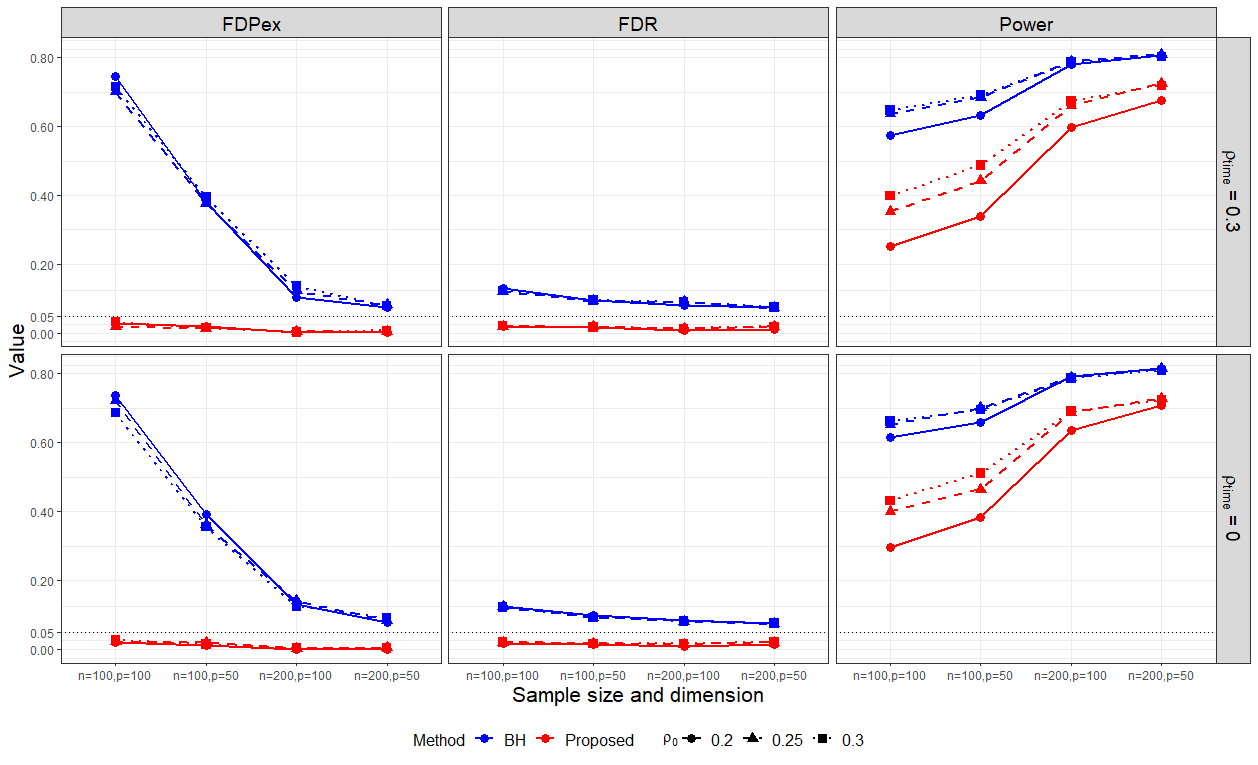
\includegraphics[width=\linewidth]{plot-correlation-block.png}
	\caption{The average FDPex rate $\mathbb{P}(\mbox{FDP} > 0.1)$, FDR and power of the proposed (red) and BH (blue) procedures for testing the hypotheses (\ref{eq:MultiATE}) to recover the nonzero treatment effects on the subject level correlations under the block-diagonal signal setting with $s_0 = 10$, $m = 300$, $n = 100, 200$, $p = 50, 100$ and $\rho_{\mathrm{\scriptstyle time}} = 0$ and $0.3$. The nominal level was $0.05$.}
	\label{simulation1}
\end{figure}

\begin{figure}[t]
	\centering
	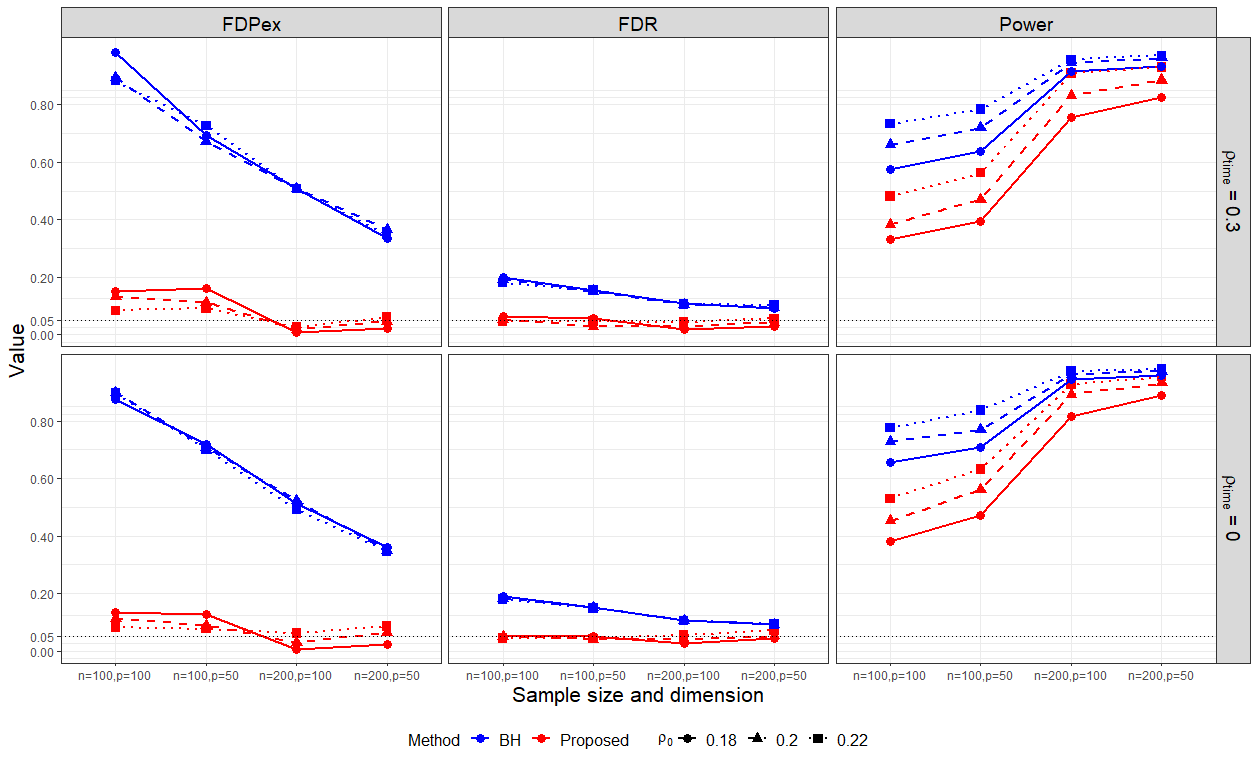
\includegraphics[width=\linewidth]{plot-correlation-off.png}
	\caption{The average FDPex rate $\mathbb{P}(\mbox{FDP} > 0.1)$, FDR and power of the proposed (red) and BH (blue) procedures for testing the hypotheses (\ref{eq:MultiATE}) to recover the nonzero treatment effects on the subject level correlations under the super-diagonal signal setting with $s_1 = 6$, $m = 300$, $n = 100, 200$, $p = 50, 100$ and $\rho_{\mathrm{\scriptstyle time}} = 0$ and $0.3$. The nominal level was $0.05$.}
	\label{simulation2}
\end{figure}


\iffalse
\begin{table}[!htb]
\scriptsize
\begin{center}
\caption{\textit{The empirical FDPex rate $\mathbb{P}(\mbox{FDP} > 0.1)$, FDR and power of the proposed and BH procedures for testing the hypotheses (\ref{eq:MultiATE}) to recover the nonzero treatment effects on the subject level correlations under the block-diagonal  setting with $s_0 = 10$, $m = 300$, $n = 100, 200$, $p = 50, 100$ and $\rho_{\mathrm{\scriptstyle time}} = 0, 0.3$. The nominal level was set as $0.05$.
}} \medskip
\label{simulation1}
\begin{tabular}{c|ccc|ccc|ccc|ccc}
\hline\hline
 & \multicolumn{12}{c}{time dependence parameter $\rho_{\mathrm{\scriptstyle time}} = 0$} 
\\ \cline{2-13} 
 & \multicolumn{6}{c|}{$p = 50, n = 100$} & \multicolumn{6}{c}{$p = 50, n = 200$}
\\ \cline{2-13} 
 & \multicolumn{3}{c|}{Proposed} & \multicolumn{3}{c|}{BH} & \multicolumn{3}{c|}{Proposed} & \multicolumn{3}{c}{BH} 
\\ \cline{2-13} 
$\rho_0$ & FDPEx & FDR & Power & FDPEx & FDR & Power & FDPEx & FDR & Power & FDPEx & FDR & Power 
\\ \hline
0.20 &0.012&0.015&0.383&0.393&0.098&0.658 &0.001&0.015&0.710&0.079&0.075&0.817
\\ \cline{2-13}
0.25 &0.020&0.016&0.464&0.361&0.093&0.700 &0.004&0.020&0.727&0.083&0.074&0.815
\\ \cline{2-13}
0.30 &0.014&0.015&0.512&0.355&0.092&0.695 &0.004&0.020&0.723&0.090&0.075&0.809
\\ \hline
 & \multicolumn{6}{c|}{$p = 100, n = 100$} & \multicolumn{6}{c}{$p = 100, n = 200$}
\\ \hline
0.20 &0.020&0.018&0.395&0.738&0.125&0.615 &0.001&0.010&0.637&0.130&0.085&0.793
\\ \cline{2-13}
0.25 &0.021&0.019&0.400&0.722&0.123&0.653 &0.003&0.015&0.688&0.140&0.080&0.789
\\ \cline{2-13}
0.30 &0.027&0.020&0.431&0.686&0.122&0.662 &0.004&0.017&0.690&0.125&0.081&0.787
\\ \hline\hline

 & \multicolumn{12}{c}{time dependence parameter $\rho_{\mathrm{\scriptstyle time}} = 0.3$} 
\\ \cline{2-13} 
 & \multicolumn{6}{c|}{$p = 50, n = 100$} & \multicolumn{6}{c}{$p = 50, n = 200$}
\\ \cline{2-13} 
 & \multicolumn{3}{c|}{Proposed} & \multicolumn{3}{c|}{BH} & \multicolumn{3}{c|}{Proposed} & \multicolumn{3}{c}{BH} 
\\ \cline{2-13} 
$\rho_0$ & FDPEx & FDR & Power & FDPEx & FDR & Power & FDPEx & FDR & Power & FDPEx & FDR & Power 
\\ \hline
0.20 &0.019&0.016&0.339&0.379&0.095&0.633 &0.001&0.011&0.676&0.074&0.075&0.805
\\ \cline{2-13}
0.25 &0.014&0.017&0.442&0.376&0.093&0.683 &0.003&0.018&0.725&0.082&0.073&0.809
\\ \cline{2-13}
0.30 &0.015&0.016&0.486&0.395&0.095&0.692 &0.007&0.018&0.719&0.079&0.075&0.803
\\ \hline
 & \multicolumn{6}{c|}{$p = 100, n = 100$} & \multicolumn{6}{c}{$p = 100, n = 200$}
\\ \hline
0.20 &0.028&0.020&0.353&0.745&0.131&0.575 &0.001&0.008&0.598&0.104&0.089&0.780
\\ \cline{2-13}
0.25 &0.018&0.019&0.353&0.700&0.121&0.636 &0.005&0.013&0.661&0.122&0.090&0.788
\\ \cline{2-13}
0.30 &0.032&0.021&0.398&0.715&0.123&0.647 &0.002&0.013&0.673&0.137&0.081&0.787
\\ \hline\hline

\end{tabular}		
\end{center}
\end{table}
\fi

\iffalse
\begin{table}[!htb]
\scriptsize
\begin{center}
\caption{\textit{The empirical FDPex rate $\mathbb{P}(\mbox{FDP} > 0.1)$, FDR and power of the proposed and BH procedures for testing the hypotheses (\ref{eq:MultiATE}) to recover the nonzero treatment effects on the subject level correlations under the super-diagonal  setting with $s_1 = 6$, $m = 300$, $n = 100, 200$, $p = 50, 100$ and $\rho_{\mathrm{\scriptstyle time}} = 0, 0.3$. The nominal level was set as $0.05$.}} \medskip
\label{simulation3}
\begin{tabular}{c|ccc|ccc|ccc|ccc}
\hline\hline
 & \multicolumn{12}{c}{time dependence parameter $\rho_{\mathrm{\scriptstyle time}} = 0$} 
\\ \cline{2-13} 
 & \multicolumn{6}{c|}{$p = 50, n = 100$} & \multicolumn{6}{c}{$p = 50, n = 200$}
\\ \cline{2-13} 
 & \multicolumn{3}{c|}{Proposed} & \multicolumn{3}{c|}{BH} & \multicolumn{3}{c|}{Proposed} & \multicolumn{3}{c}{BH} 
\\ \cline{2-13} 
$\rho_0$ & FDPEx & FDR & Power & FDPEx & FDR & Power & FDPEx & FDR & Power & FDPEx & FDR & Power 
\\ \hline
0.18 &0.126&0.050&0.472&0.719&0.154&0.707 &0.024&0.042&0.888&0.362&0.092&0.960
\\ \cline{2-13}
0.20 &0.088&0.039&0.561&0.709&0.151&0.769 &0.065&0.052&0.932&0.349&0.092&0.972
\\ \cline{2-13}
0.22 &0.077&0.043&0.632&0.702&0.148&0.838 &0.086&0.071&0.953&0.347&0.092&0.980
\\ \hline
 & \multicolumn{6}{c|}{$p = 100, n = 100$} & \multicolumn{6}{c}{$p = 100, n = 200$}
\\ \hline
0.18 &0.134&0.051&0.382&0.874&0.190&0.655 &0.007&0.028&0.815&0.514&0.107&0.945
\\ \cline{2-13}
0.20 &0.112&0.050&0.452&0.900&0.183&0.730 &0.030&0.041&0.892&0.524&0.107&0.962
\\ \cline{2-13}
0.22 &0.082&0.044&0.530&0.897&0.179&0.776 &0.062&0.056&0.928&0.492&0.105&0.973
\\ \hline\hline

 & \multicolumn{12}{c}{time dependence parameter $\rho_{\mathrm{\scriptstyle time}} = 0.3$} 
\\ \cline{2-13} 
 & \multicolumn{6}{c|}{$p = 50, n = 100$} & \multicolumn{6}{c}{$p = 50, n = 200$}
\\ \cline{2-13} 
 & \multicolumn{3}{c|}{Proposed} & \multicolumn{3}{c|}{BH} & \multicolumn{3}{c|}{Proposed} & \multicolumn{3}{c}{BH} 
\\ \cline{2-13} 
$\rho_0$ & FDPEx & FDR & Power & FDPEx & FDR & Power & FDPEx & FDR & Power & FDPEx & FDR & Power 
\\ \hline
0.18 &0.135&0.059&0.396&0.694&0.153&0.639 &0.021&0.030&0.825&0.336&0.092&0.933
\\ \cline{2-13}
0.20 &0.113&0.028&0.470&0.673&0.151&0.719 &0.046&0.043&0.885&0.366&0.095&0.963
\\ \cline{2-13}
0.22 &0.092&0.047&0.563&0.727&0.154&0.784 &0.060&0.056&0.930&0.350&0.102&0.971
\\ \hline
 & \multicolumn{6}{c|}{$p = 100, n = 100$} & \multicolumn{6}{c}{$p = 100, n = 200$}
\\ \hline
0.18 &0.151&0.065&0.332&0.984&0.210&0.577 &0.008&0.019&0.756&0.509&0.108&0.917
\\ \cline{2-13}
0.20 &0.134&0.054&0.382&0.895&0.193&0.660 &0.018&0.028&0.831&0.509&0.105&0.945
\\ \cline{2-13}
0.22 &0.084&0.045&0.481&0.883&0.180&0.733 &0.027&0.043&0.909&0.507&0.106&0.957
\\ \hline\hline

\end{tabular}		
\end{center}
\end{table}
\fi

From Figures \ref{simulation1} and \ref{simulation2}, we observe that the proposed method can control the FDPex rate for testing the hypotheses (\ref{eq:MultiATE}) smaller than 0.05 under most of the cases, except for the super-diagonal signal setting under $n = 100$, where the FDPex rate was around 0.1. But this error rate decreased to less than 0.05 when the number of subjects $n$ was increased to $200$.
Meanwhile, the FDR of the proposed method was well controlled, around 5\% under all the cases. 
In comparison, the empirical FDPex rate of the BH procedure was quite large, which reached over 0.7 and 0.9 under the block-diagonal and super-diagonal signal settings with $n = 100$, respectively.
The FDPex rate of BH became much smaller under the block-diagonal setting when $n$ was increased to $200$, but it was still larger than 5\%. 
This shows that the BH procedure can not control the FDP exceedance rate for testing many treatment effects derived from the same group of subjects.
Also, notice that BH encountered a slight inflation on FDR. Its FDR was around 0.1 larger than the nominal level 5\%. 
It reached around 0.2 under the super-diagonal setting and $n = 100$. 
This may be due to the dependence among the estimated treatment effects $\{\hat{\tau}_j\}$ in (\ref{eq:EstATE1}) as they all use the common propensity scores.

%the empirical FDR of BH procedure exceed 0.05 in all settings and is larger than 0.1 when sample size is small or dimension of observation is large. The FDP exceedance rate of BH procedure can’t be controlled in most settings. The FDP exceedance rate is significantly reduced by our procedure compared to the BH procedure. Meanwhile, FDR is also controlled at a low value, which outperforms the BH method because BH method does not take the dependence in estimation into account.
%In super diagonal setting, the results are alike. The difference is that the FDP exceedance rate of BH procedure is very large, even with large sample size and small observation dimension. Though the FDP exceedance rate of our method is not controlled under 0.05 when sample size is small, it is still much smaller than BH method. We also notice that when sample size is large, the FDR and FDP exceedance rate are both well-controlled by our method.

The overall power of the proposed test was reasonable, and it was much increased with the increase of the sample size from $100$ to $200$. Compared with the BH procedure, the power of the proposed procedure was lower, especially under $n = 100$. 
This is because of the size inflation of the BH procedure and the more stringent Type I error control of our procedure. Notice that both procedures use the same estimates of the average treatment effects. The difference is solely from the ways of choosing the cut-off value for testing the multiple hypotheses (\ref{eq:MultiATE}).
When $n$ was increased to $200$, the power of the proposed procedure became much closer to those of BH. Especially, under the super-diagonal setting and $n = 200$, the power of both methods reached around 0.9.
Also notice that the results under $\rho_{\mathrm{\scriptstyle time}} = 0$ and $\rho_{\mathrm{\scriptstyle time}} = 0.3$ were comparable for both methods. When $\rho_{\mathrm{\scriptstyle time}} = 0$, the subject level data were temporally independent. 
The power under $\rho_{\mathrm{\scriptstyle time}} = 0.3$ was slightly lower, which was due to the larger variation of the estimated subject level correlations under time-dependent data.  


%The average true positive rate (TPR) is lower in our procedure than BH procedure, which is because we have to delete those findings with low p-value in BH method to control FDR and FDP exceedance rate. To take the dependence of estimation into account to control FDP exceedance rate, the decrease of true positive rate is unavoidable. However, this is a necessary cost because if a true discovery is mixed with multiple false discoveries, we are not able to find which discovery is of real value. Also, the decrease of TPR is not too much when the sample size is large, while the decrease of FDP exceedance rate is significant even when n is large as can be seen in Table \ref{simulation3} and Table \ref{simulation4}.
%The ability to control FDR and FDP exceedance rate is not largely affected by the sample size, though the outcome may slightly exceed $\alpha$ in the second setting. However, sample size can significantly affect the performance of tpr in our method. If the sample size is not adequate, the FDR of our method may be much lower than BH method. As a result, we recommend to use our procedure when the sample size is not small.

%The existence of dependence over repeated measurements does not affect the ability to control FDR and FDP exceedance rate, but may leads to slight decrease of TPR. This is consistent with our expectations. Performance under different $\rho_0$ is very much alike because the ratio of absolute causal effect and $\rho_0$ is a constant no matter what value $\rho_0$ takes. This is also consistent with our expectation. Finally, it can also be seen that larger dimension p does not affect FDR and FDP exceedance rate a lot but will result in lower TPR bacuase the higher dimension p is, the more parameters we have to estimate, which means more variations.

%In conclusion, in most settings of our simulation, FDR and FDP exceedance rate is well-controlled by our procedure, which performs much better than traditional BH method. Though our method may lead to some decrease of TPR as a cost for controlling FDR, the decrease is not large when sample size is adequate compared to BH method. As a result, our procedure is beneficial in controlling FDP exceedance rate in causal discoveries.

To evaluate the treatment effects on regression coefficients in Example 2, 
we compared the performance of the proposed method with the lasso estimate and the de-sparsified lasso estimate described in Section S1 in the SM.
Note that the lasso estimate is biased, which does not satisfy Condition \ref{as:est}. 
The covariates $\bW_i$, treatment assignment $D_i$ and the subject level covariance matrix $\bY_i(0)$ under control were generated the same as the simulation settings for Example 1. Let $\bOmega_{i}(d) = (\omega_{i, j_1j_2}(d)) = \bY_i^{-1}(d)$ be the precision matrix. 
We added the signals on $\bOmega_{i}(1)$ in the block-diagonal setting where 
$\omega_{i, j_1j_2}(1) = \omega_{i, j_1j_2}(0) + \rho_{0}|\delta_{i}| $ for $(j_1, j_2) \in \mathcal{S}_{\mathrm{\scriptstyle bd}}$ and $\omega_{i, j_1j_2}(1) = \omega_{i, j_1j_2}(0)$ for $(j_1, j_2) \not\in \mathcal{S}_{\mathrm{\scriptstyle bd}}$.
The subject level data $\bX_{i, t}$ were generated by the VAR model with the error distribution $N({\bf 0}, \bOmega_{i}^{-1})$, where $\bOmega_{i} = D_{i}\bOmega_{i}(1) + (1 - D_{i}) \bOmega_{i}(0)$.
From Example 2, the support of the coefficients $\{Y^{\ast}_{i, j_1j_2}(d)\}$ of the nodewise regressions is the same as that of the precision matrix $\bOmega_{i}(d)$.
The lasso penalty parameters $\lambda_{j}$ and $\lambda_{j_1j_2}$ were set as $\sqrt{2(\log p) / m}$ for all $j, j_1, j_2$.

The average FDPex rate, FDR and power are reported in Figure S1 in the SM. We observe that the proposed method with the de-sparsified lasso estimate was able to control the FDPex rate under the nominal level 5\% with good power. Its FDR was also controlled at 5\%.
In contrast, the proposed method with the lasso estimate failed to work. Its power was lower than 0.1 for all the cases due to the underestimation of the true regression coefficients. 
These results show that the asymptotic unbiasedness condition (Condition \ref{as:est}) is essential for the validity of the proposed method. Simply using any consistent estimator for the subject level parameters 
%or treat the derived outcomes as the outcome of interest without accounting for their uncertainty 
may not lead to desirable estimates of the treatment effects.

%In the second simulation, we considered the treatment effects on regression coefficients in Example 2 in Section~\ref{se:background} and hypotheses (\ref{eq:MultiATE}). We compare the performance of the lasso estimate (without bias correction) and the de-sparsified lasso estimate (de-biased estimate) described in Section \ref{se:de-bias}.

%\textcolor{red}{The data generating procedure is exactly the same as the block-diagonal setting described in Simulation One, except that treatment effects of strength $\rho_{0}|\delta_{i}|$ now appear in the blocks along the main diagonal of the precision matrix instead of the correlation matrix. Under the block-diagonal setting, the nonzero treatment effects appear in the blocks of size $s_0$ along the main diagonal of the precision matrices. There are no causal effects on subject level regression coefficients outside those blocks.}

%\textcolor{red}{The simulation parameter settings are the same as those in Simulation One. For the proposed multiple testing procedure, we aimed to control the FDPex rate over 0.1 at 0.05, namely, $\mathbb{P}(\mbox{FDP} > 0.1) \leq 0.05$. For the lasso estimate, we set the penalty parameter $\lambda_j$ to be $\sqrt{\frac{2log(p)}{n}}$ for each j. For the de-sparsified lasso estimate, we set the penalty parameter $\lambda_{j_1j_2}$ to be $\sqrt{\frac{2log(p)}{n}}$ for each $j_1$ and $j_2$. Note that the lasso estimate does not satisfy the asymptotic unbiasedness condition (Condition \ref{as:est}). Though it is a consistent estimator, it is biased and can not be used to infer the population treatment effect. The average FDR, FDPex proportion and empirical power of the two methods are reported in Figure \ref{simulation3}.}

\iffalse
\begin{figure}[t]
	\centering
	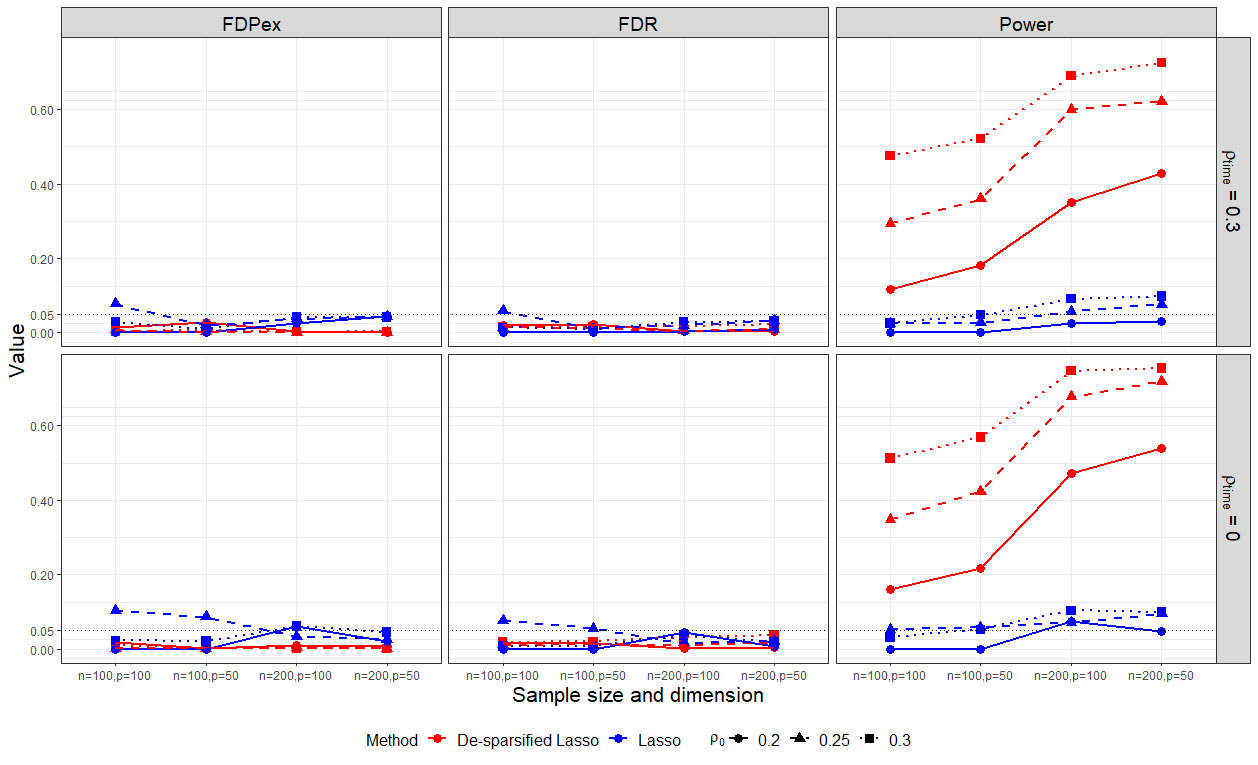
\includegraphics[width=6in]{plot-regression-block.png}
	\caption{The empirical FDPex rate $\mathbb{P}(\mbox{FDP} > 0.1)$, FDR and power of the de-biased lasso and regular lasso for testing the hypotheses (\ref{eq:MultiATE}) to recover the nonzero treatment effects on the subject level regression coefficients under the block-diagonal  setting with $s_0 = 10$, $m = 300$, $n = 100, 200$, $p = 50, 100$ and $\rho_{\mathrm{\scriptstyle time}} = 0, 0.3$. The nominal level was set as $0.05$.}
	\label{simulation3}
\end{figure}
\fi

%\textcolor{red}{From Figure \ref{simulation3}, we observe that the both methods can control the FDPex rate and FDR for testing the hypotheses (\ref{eq:MultiATE}) smaller than 0.05 under most of the cases. However, the estimated ATEs using the lasso estimator have very low power in detecting nonzero treatment effects, while the estimates using the de-biased estimator have much higher power. The power of the de-biased lasso can reach 0.75 when $n=200$ and $p=50$ while the power of the lasso estimator is smaller than 0.1 in most of the cases. The results show that the asymptotic unbiasedness condition (Condition \ref{as:est}) is essential for the correct use of the proposed method. Simply use some kind of consistent estimates of the subject level parameters or treat the derived outcomes as the outcome of interest without accounting for their uncertainty would lead to unreliable conclusions.}


\setcounter{equation}{0}
\section{Case study}\label{se:case-study}

It is well recognized that neurodevelopmental and neurodegenerative disorders, like Autism spectrum disorder (ASD), are associated with altered patterns of over- and under-connectivity in brains \citep{kana2014brain}.
In this section, we studied medication effects on the brain functional connectivity of patients with ASD. 
%It is believed that neurodevelopmental and neurodegenerative disorders, like Autism spectrum disorder (ASD), 
We used the fMRI data of 79 ASD patients from New York University Langone Medical Center. 
The preprocessed data were downloaded from the Autism Brain Imaging Data Exchange I initiative \citep{craddock2013neuro}.
%\citep{di2014autism}, and were preprocessed by the C-PAC pipeline \citep{craddock2013neuro}. See the details of the preprocessing steps at the ``ABIDE Preprocessed'' website. 
Among the 79 patients, 16 of them had taken some kind of medications for alleviating the related symptoms of ASD, and the rest 60 had not. 
We estimated and identified the nonzero treatment effects on brain functional connectivity, measured by correlations among brain regions, between the groups taking and not taking medications within three months before taking fMRI scans. 
%by identifying the nonzero population average treatment effect. 

For each subject, there were 175 scans of brain overtime in the fMRI data, and  
%According to the official website of ABIDE I, the scan data is preprocessed (detail of preprocession can be seen on the official website \url{http://preprocessed-connectomes-project.org/abide/Pipelines.html#min_preproc}) and 
a set of 116 regions-of-interests (ROI) were extracted according to the automated anatomical labeling atlas. 
%\citep{tzourio2002automated}. 
Following 
%the software BrainNet Viewer \citep{xia2013brainnet} and 
\cite{liu2020alterations}, those 116 ROIs can be divided into six common functional networks: the default mode network (DMN), the execution and attention network (EAN), the sensorimotor network (SMN), the visual network (Visual), the subcortical nuclei (SBN) regions and the cerebellum (Cerebel), which consist of 22, 17, 18, 14, 19, 26 regions, respectively. Data of three patients were deleted, one of which was due to missing covariates and the other two were due to missing values in the ROIs. The final data included 76 ASD patients. 
%There are 16 ASD patients who take medicine and 60 not.

Four covariates including age, sex, handedness and FIQ were chosen in the analysis. Age and sex are binary variables, handedness is an integer score between -100 and 100 with a higher score implying more use of the right hand and vice versa, and FIQ is a positive integer score representing the standard estimate of intelligence. 
%According to CDC \citep{CDC}, 
Note that the development of ASD symptoms is related to age, and ASD is a disorder of sexual differentiation \citep{alaerts2016sex}. 
IQ scores also affect the decision of taking medicine. An ASD patient may be treated if there is some abnormality in IQ. Meanwhile, those covariates are also related to the differences in brain connectivity among subjects. 
Therefore, age, sex and IQ can be regarded as common causes for the treatment indicator and the potential responses.
%taking medications and the differences in brain connectivity.
We make the unconfoundedness assumption that the treatment assignment and the potential fMRI readings are conditionally independent given the covariates. 
%the indicator variable D for taking medicine and the potential outcomes of ROI connectivities given the covariates W. 
%Apparently, taking medicine or not will be affected by age and sex. If a child is too young, taking medicine may not be suggested, for example. Since age and sex affect both ASD and brain connectivity, we can regard them as common causes of the difference in ROI connectivity and gaining of ASD. On the other hand, IQ and ROI connectivity of ASD patients are both decided by gene, and IQ can affect whether an ASD child takes medicine. An ASD child may be treated if he has some abnormality in IQ. In conclusion, unconfoundedness assumption is reasonable since covariate W consist of common causes for treatment indicator and the potential outcomes and variable which lies on the way between common cause and treatment.

We applied the proposed procedure for testing the multiple hypotheses (\ref{eq:MultiATE}) to identify the nonzero treatment effects on the subject level correlations among brain ROIs. Similar to the simulation study, we controlled the probability of FDP exceeding 0.1 at 0.05, namely, $c = 0.1$ and $\alpha = 0.05$. 
We discovered 4 significant pairs of brain connections 
%associated with 8 ROIs. Those identified pairs of ROIs 
with nonzero ATE of medication on ASD patients, which are reported in Table \ref{ROIcausal} together with the corresponding functional network. 
The BH procedure that controls the FDR at 5\% based on the standardized estimated treatment effects gives the same set of discovered connections as the proposed method for this data set.
The estimated treatment effects for the 4 discovered pairs, their 95\% confidence intervals, the IPW averages for the treatment and control groups, $n^{-1}\sum_{i = 1}^{n} {\hat{Y}_{i, j}D_{i}} / {\Lambda(\bW_{i}^{\T}\hat{\bbeta})}$ and
%and the IPW averages for the control group, 
$n^{-1}\sum_{i = 1}^{n} {\hat{Y}_{i, j}(1 - D_{i})} / \{1 - \Lambda(\bW_{i}^{\T}\hat{\bbeta})\}$, are also reported in Table \ref{ROIcausal}.
The visualization of those connections is shown in Figure S2 in the SM. 
%The Figure is plotted using the software  the BrainNet Viewer \citep{xia2013brainnet}.
All six functional networks except the cerebellum network were involved in those significant connections. 
Notice that the correlation between SMA.L and HES.R were altered in the positive direction on average by medication, while the correlations of the other three pairs were negatively enhanced. 
Among the identified ROIs, HES.R was also reported to be strongly associated with the severity of ASD in \cite{liu2020alterations}.
%They contribute to $80\%$ of the discovered connections, which was previously reported in \cite{liu2020alterations}. The ROIs related to language systems, such as the superior temporal gyri (STG.L(81), STG.R(82)), the middle temporal gyri (MTG.L(85), MTG.R(86)) are strongly associated with the discovered connections, and this was also mentioned in \cite{liu2020alterations}. 
%An interesting discovery is that 
The discovered connections were mainly related to the execution and attention network (EAN). According to CDC, signs and symptoms of ASD 
%include difficulties in social communication and interaction skills, restricted or repetitive behaviors or interests, inattentive behavior and other behaviors that 
are associated with execution and attention.
\cite{bernas2018brain, snyder2020behavioural} also found evidence that relates the abnormalities of neurodynamics and connectivity of ASD brains to brain regions associated with attention and execution.
Our method reveals the medication effects on brain connectivities of some regions in EAN, which may alleviate the symptoms of ASD.

%\textcolor{red}{In previous literature, \cite{bernas2018brain} finds that there is a difference between high-functioning autism and controls in the temporal neurodynamics from the ventral attention network to the salience-executive network. It is also reported in \cite{snyder2020behavioural} that hyperconnectivity in ASD brains is significantly related to attention and execution, and that hypoconnectivity is related to execution behaviors. As a result, our method may reveal the fact that the medicine has an effect on the brain connectivities that are related to execution and attention behaviors for ASD patients to lessen the symptoms and cure the disease.}

%As a result, our method may reveal the effectiveness of medicine on improving the EAN connections of ASD patients, which could lead to the alleviation of symptoms.

\begin{table}[t]
\footnotesize
\begin{center}
\caption{\textit{The four pairs of ROIs (the functional networks they belong to in the parentheses) with the identified nonzero treatment effects on subject level correlations by the proposed multiple testing procedure, the estimated treatment effect, its 95\% confidence interval, and the IPW averages for the treatment group (Ave-trt) and the control group (Ave-cl). 
%are reported in the third to sixth columns, respectively. 
%Population level brain connectivity difference discovered by the multiple testing procedure of causal method. Fisrt and third columns are the names of the related ROIs. Second and Fourth columns are the functional networks they belong to.
}} \medskip
\label{ROIcausal}
		%	\begin{tabular}{c|cc|cc}
		%		\hline
		%		Number & ROI1 Name       & ROI1 Network       & ROI2 Name      & ROI2 Network            \\ \hline
		%		1      & Putamen-R       & Subcortical Nuclei & Frontal-Mid-R  & Execution and Attention \\ \hline
		%		2      & Pallidum-L      & Subcortical Nuclei & Frontal-Mid-R  & Execution and Attention \\ \hline
		%		3      & Rolandic-Oper-R & Sensorimotor       & Pallidum-L     & Subcortical Nuclei      \\ \hline
		%		4      & Hippocampus-R   & Subcortical Nuclei & Temporal-Mid-R & Default Mode            \\ \hline
		%		5      & Hippocampus-R   & Subcortical Nuclei & Temporal-Inf-R & Default Mode            \\ \hline
		%		6      & Putamen-L       & Subcortical Nuclei & Cerebelum-9-L  & Cerebellum              \\ \hline
		%		7      & Pallidum-L      & Subcortical Nuclei & Temporal-Sup-L & Sensorimotor            \\ \hline
		%		8      & Pallidum-L      & Subcortical Nuclei & Temporal-Sup-R & Sensorimotor            \\ \hline
		%		9      & Pallidum-R      & Subcortical Nuclei & Temporal-Sup-R & Sensorimotor            \\ \hline
		%		10     & Thalamus-L      & Subcortical Nuclei & Temporal-Mid-L & Default Mode            \\ \hline
		%		11     & Thalamus-R      & Subcortical Nuclei & Temporal-Mid-R & Default Mode            \\ \hline
		%	\end{tabular}
		
\begin{tabular}{ccccccc}
\hline\hline
 & ROI$_1$ (Network) & ROI$_2$ (Network) & Estimated effect & 95\% CI & Ave-trt & Ave-cl  \\ \hline
1 & SMA.L (EAN) & HES.R (SMN) & 0.164 & (0.098, 0.230) & 0.136 & -0.029 \\
2 & IPL.L (EAN) & CAU.R (SBN) & -0.138 & (-0.198, -0.077) & -0.264 & -0.126 \\
3 & IPL.R (EAN) & ITG.L (EAN) & -0.187 & (-0.262, -0.111) & -0.231 & -0.044 \\
4 & ORBsup.L (DMN) & MOG.L (Visual) & -0.163 & (-0.233, -0.094) & -0.217 & -0.053 \\ 
\hline\hline
\end{tabular}		
\end{center}
\end{table}

\iffalse
\begin{figure}[t]
	\centering
	
	\subfigure[Axial]{
		\begin{minipage}[t]{0.45\linewidth}
			\centering
			\includegraphics[width=3in]{Brain_Axial_causal.png}
		\end{minipage}
	}
	\subfigure[Coronal]{
		\begin{minipage}[t]{0.45\linewidth}
			\centering
			\includegraphics[width=3in]{Brain_Coro_causal.png}
		\end{minipage}
	}
	\caption{Pairs of ROIs with significant treatment effects of medication on brain functional connectivity of ASD patients, measured by correlations among ROIs, by the proposed multiple testing procedure. Colors of nodes represent the functional networks they belong to.
	%SMN (red), Visual (orange), EAN (green), DMN (sky blue), SBN (purple) and Cerebellum (pink).
	}
	\label{Causalconnection}
\end{figure}
\fi

%\begin{figure}[H]
%	\centering
	
%	\subfigure[Axial]{
%		\begin{minipage}[t]{0.45\linewidth}
%			\centering
%			\includegraphics[width=3in]{Brain_Axial_correlation.png}
%		\end{minipage}
%	}
%	\subfigure[Coronal]{
%		\begin{minipage}[t]{0.45\linewidth}
%			\centering
%			\includegraphics[width=3in]{Brain_Coro_correlation.png}
%		\end{minipage}
%	}
%	\caption{Significant difference of brain functional connectivity between normal people and people with Autism spectrum disorder discovered by the Multiple testing procedure through correlation method. Colours of nodes imply the common functional networks they belong to. The corresponding relationship between color serial number and networks are: Network 1: SMN; Network 2: Visual; Network 3: EAN; Network 4: DMN; Network 5: SBC; Network 6: Cerebellum.}
%	\label{Correlationconnection}
%\end{figure}

%The BH procedure that controls the FDR at 5\% based on the standardized estimated treatment effects gives the same set of discovered connections as the proposed method for this data set.
We also applied the two-sample t-test directly on the subject level sample correlations $\{\hat{Y}_{i, j_1j_2}\}$. 
%without adjusted by the estimated propensity scores. 
This is equivalent to treating the propensity score in (\ref{eq:EstATE1}) being 16/76 for all subjects, as the ratio of the number of treated patients over the total sample size. 
Such a procedure is commonly used in many neuroscience studies.
%to test for the differences in the average correlations of the two groups.
However, no significant difference in correlations between the treatment and control groups was found without the propensity score adjustment. This shows that simply conducting two-sample t-tests may not be able to identify treatment effects in observational studies for brain connectivity.
%We also use population average correlation difference to replace the ATE in the Multiple testing procedure to identify population level brain connectivity through correlation method in place of causal method. However, no difference in connection is found by the correlation method. As ATE reveals the true effect of treatment on brain connections while population average correlation difference represents only correlation, which may be affected by confoundings that are not adjusted, we believe that causal method gives a better way to discover difference in brain connections.
%find 8 connections associated with 13 ROIs. The detailed results are displayed in Figure \ref{Correlationconnection} and Table \ref{ROIcorrelation}.

% The causal method finds significantly different connections while correlation method not. 
 
% Half of the discoveries are the same while the others are different. The discovery of causal findings are mainly among the connections between the default mode network (DMN), the sensorimotor network (SMN) and the subcortical nuclei (SBN) regions, while the findings of correlation method are mainly among the execution and attention network (EAN), the default mode network (DMN) and the subcortical nuclei (SBN) regions. The discovered connections of causal method are more concentrated since they are all inter-network connections between the subcortical nuclei (SBN) regions and other networks while the discovery of correlation method is more apart, including inter-network and intra-network connections among EAN, DMN and SBN regions. Since previous report such as \cite{alaerts2016sex} shows that population with different covariates like sex can show a differential neural expression of ASD, it is reasonable to consider that the causal method can better reveal the true effect of ASD on brain connections.

%\begin{table}[H]
%	\footnotesize
%	\begin{center}
%		\caption{\textit{Population level brain connectivity difference discovered by the multiple testing procedure of correlation method. Fisrt and third columns are the names of the related ROIs. Second and Fourth columns are the functional networks they belong to.}} \medskip
%		\label{ROIcorrelation}
%\begin{tabular}{c|cc|cc}
%	\hline
%	Number & ROI1 Name            & ROI1 Network            & ROI2 Name         & ROI2 Network            \\ \hline
%	1      & Frontal-Mid-Orb-L    & Execution and Attention & Temporal-Inf-L    & Execution and Attention \\ \hline
%	2      & Frontal-Inf-Tri-R    & Execution and Attention & Frontal-Med-Orb-L & Default Mode            \\ \hline
%	3      & Frontal-Sup-Medial-R & Default Mode            & Frontal-Med-Orb-L & Default Mode            \\ \hline
%	4      & Frontal-Med-Orb-R    & Default Mode            & Cingulum-Ant-R    & Default Mode            \\ \hline
%	5      & Hippocampus-R        & Subcortical Nuclei      & Temporal-Mid-R    & Default Mode            \\ \hline
%	6      & Hippocampus-R        & Subcortical Nuclei      & Temporal-Inf-R    & Default Mode            \\ \hline
%	7      & Thalamus-L           & Subcortical Nuclei      & Temporal-Mid-L    & Default Mode            \\ \hline
%	8      & Thalamus-R           & Subcortical Nuclei      & Temporal-Mid-R    & Default Mode            \\ \hline
%\end{tabular}
		
%	\end{center}
%\end{table}


\setcounter{equation}{0}
\section{Discussion}\label{se:discussion}

In this paper, we consider estimating the ATEs of unobservable random variables from each subject under the ignorability assumption. Those unobservable random variables need to be estimated using subject level data. 
Our theoretical analysis shows that an additional unbiasedness condition is needed for the identifiability and estimation of the ATEs, compared with the classical causal inference problems under the ignorability assumption.
This implies that not all consistent estimators of the subject level parameters of interest can be used to estimate the population treatment effects. A de-biased estimator satisfying Condition \ref{as:est} needs to be constructed. 

We study the treatment effects on brain functional connectivity measured by Pearson’s correlation in the case study. 
The proposed method can be applied to other measures of brain connectivity, for example, Spearman’s $\rho$ and Kendall’s $\tau$ for nonlinear association and partial correlation for conditional association. 
The proposed procedure can be extended to dynamic treatment effects over time as well, where the subject level potential outcomes $\bY_i(d, t)$ and the average treatment effects $\btau(t) = {\E}\{\bY_{i}(1, t) - \bY_{i}(0, t)\}$ are functions of time \citep{bojinov2021panel}.
This setting is suitable for task-based fMRI data where the brain activity patterns are likely to change with respect to the given tasks. 
Developing more powerful multiple testing procedures able to control the FDP under a general dependence structure among the estimated ATEs is also worth investigating in future work.
%In this case, to construct simultaneous confidence region for the treatment effect function $\btau(t)$ over a period of time, we also need to account for the subject level temporal dependence.

\iffalse

\section{Appendix}

Let $C$ be a positive constant which may change from case to case. Let $|\ba|_{\infty} = \max_{j} |a_j|$ for a vector $\ba = (a_1, \ldots, a_p)^{\T}$, and $|\bA|_{\infty} = \max_{j_1, j_2} |a_{j_1j_2}|$ for a matrix $\bA = (a_{j_1j_2})$, which denotes 
%the vector maximum norm for vectors and 
the element-wise maximum norm for vectors and matrices. 

\noindent{\bf Proof of Proposition \ref{pn:1}.}
%Notice that the double subscripts $j_{1}j_{2}$ is used in $Y_{i, j_1j_2}$ and $\tau_{j_1j_2}$ to denote the correlation between $j_1$th and $j_2$th variable in Example 1.
%Here, to unify the notation, we simply use $\hat{Y}_{i, j}$ to denote the $j$th component of $\hat{Y}_{i}$. 
Recall that  $\dot{\rho}_{\beta}(\bW_{i}, D_{i}) = \{D_{i} - \Lambda(\bW_{i}^{\T}\beta)\} \bW_{i}$ is the first derivative of the log likelihood function of the logistic regression, and $\bXi_{\beta_{0}}$ is the inverse of its Fisher information matrix at the true parameter $\bbeta_0$. The MLE $\hat{\bbeta}$ can be expanded as
\begin{equation}
\sqrt{n}\big(\hat{\bbeta} - \bbeta_{0}\big) = \bXi_{\beta_{0}}\frac{1}{\sqrt{n}}\sum_{i=1}^{n}\dot{\rho}_{\beta_{0}}(\bW_{i},D_{i}) + O_{p}(n^{-1/2}).\label{eq:debiasLasso1}
\end{equation}
For each $j$, we can decompose ${\hat{Y}_{i, j}D_{i}} / {\Lambda(\bW_{i}^{\T}\hat{\bbeta})}$ as
\bea
%\frac{\hat{Y}_{i, j_1j_2}D_{i}}{g(\bW_{i}^{\T}\hat{\bbeta})} &=& 
&& \frac{\hat{Y}_{i, j}D_{i}}{\Lambda(\bW_{i}^{\T}\hat{\bbeta})} - \frac{\hat{Y}_{i, j}D_{i}}{\Lambda(\bW_{i}^{\T}\bbeta_{0})} + \frac{\hat{Y}_{i, j}D_{i}}{\Lambda(\bW_{i}^{\T}\bbeta_{0})^{2}}\{\Lambda(\bW_{i}^{\T}\hat{\bbeta}) - \Lambda(\bW_{i}^{\T}\bbeta_{0})\} \label{eq:decomp1} \\
&-& \frac{\hat{Y}_{i, j}D_{i}}{\Lambda(\bW_{i}^{\T}\bbeta_{0})^{2}}\{\Lambda(\bW_{i}^{\T}\hat{\bbeta}) - \Lambda(\bW_{i}^{\T}\bbeta_{0})\} + \frac{\hat{Y}_{i, j}D_{i}}{\Lambda(\bW_{i}^{\T}\bbeta_{0})} \{1 - \Lambda(\bW_{i}^{\T}\bbeta_{0})\} \bW_{i}^{\T}(\hat{\bbeta} - \bbeta_{0}) \ \ \ \ \ \ \label{eq:decomp2} 
\eea
\bea
&-& \frac{\hat{Y}_{i, j}D_{i}}{\Lambda(\bW_{i}^{\T}\bbeta_{0})} \{1 - \Lambda(\bW_{i}^{\T}\bbeta_{0})\} (\bW_{i}^{\T}\hat{\bbeta} - \bW_{i}^{\T}\bbeta_{0}) \nn \\
&& \ \ \ \ \ \ \ \ \ \ \ \ \ + \ \frac{1}{n}\sum_{k = 1}^{n}  \frac{\hat{Y}_{i, j}D_{i}}{\Lambda(\bW_{i}^{\T}\bbeta_{0})} \{1 - \Lambda(\bW_{i}^{\T}\bbeta_{0})\} \bW_{i}^{\T} 
\bXi_{\beta_{0}}\dot{\rho}_{\beta_{0}}(\bW_{k},D_{k})
%\mathcal{I}^{-1} \ell^{(1)}(D_{k}, \bW_{k}, \beta_{0}) 
\label{eq:decomp3} \\
&+& \frac{\hat{Y}_{i, j}D_{i}}{\Lambda(\bW_{i}^{\T}\bbeta_{0})} - \frac{1}{n}\sum_{k = 1}^{n}  \frac{\hat{Y}_{i, j}D_{i}}{\Lambda(\bW_{i}^{\T}\bbeta_{0})} \{1 - \Lambda(\bW_{i}^{\T}\bbeta_{0})\} \bW_{i}^{\T} 
\bXi_{\beta_{0}}\dot{\rho}_{\beta_{0}}(\bW_{k},D_{k})
%\mathcal{I}^{-1} \ell^{(1)}(D_{k}, \bW_{k}, \beta_{0}). 
\label{eq:decomp4}
\eea
Since $Y_{i,j}$ and $\bW_{i}^{\T}\bbeta_{0}$ are bounded for all $i$ and $j$, 
by Taylor expansion and the expansion of $\hat{\bbeta}$ from (\ref{eq:debiasLasso1}), it can be shown that (\ref{eq:decomp1}), (\ref{eq:decomp2}) and  (\ref{eq:decomp3}) are uniformly bounded at the order $O_p(n^{-1})$ for all $i = 1, \ldots, n$ and $j = 1, \ldots, p_0$.
%(\ref{eq:MLEExpansion}).
This leads to 
$$\frac{\hat{Y}_{i, j}D_{i}}{\Lambda(\bW_{i}^{\T}\hat{\bbeta})} = \frac{\hat{Y}_{i, j}D_{i}}{\Lambda(\bW_{i}^{\T}\bbeta_{0})} - \frac{1}{n}\sum_{k = 1}^{n} \frac{\hat{Y}_{i, j}D_{i}}{\Lambda(\bW_{i}^{\T}\bbeta_{0})} \{1 - \Lambda(\bW_{i}^{\T}\bbeta_{0})\} \bW_{i}^{\T} 
\bXi_{\beta_{0}}\dot{\rho}_{\beta_{0}}(\bW_{k},D_{k}) + O_{p}(n^{-1})$$
uniformly for all $i$ and $j$.
Similar result also holds for $\hat{Y}_{i, j}(1 - D_{i}) / \{1 - \Lambda(\bW_{i}^{\T}\bbeta_{0})\}$.
Therefore,
\bea
%&&
%\frac{1}{n}\sum_{i = 1}^{n}\bigg\{\frac{\hat{Y}_{i, j}D_{i}}{\Lambda(\bW_{i}^{\T}\hat{\bbeta})} - \frac{\hat{Y}_{i, j}(1 - D_{i})}{1 - \Lambda(\bW_{i}^{\T}\hat{\bbeta})}\bigg\} \nn \\
\hat{\tau}_{j} = 
\frac{1}{n}\sum_{i = 1}^{n}\bigg\{\frac{\hat{Y}_{i, j}D_{i}}{\Lambda(\bW_{i}^{\T}\bbeta_{0})} - \frac{\hat{Y}_{i, j}(1 - D_{i})}{1 - \Lambda(\bW_{i}^{\T}\bbeta_{0})}\bigg\} - \hat{\mathcal{H}}_{j} \frac{1}{n}\sum_{k = 1}^{n} \bXi_{\beta_{0}}\dot{\rho}_{\beta_{0}}(\bW_{k},D_{k}) + O_{p}(n^{-1}), \nn
\eea
where 
$$\tilde{\mathcal{H}}_{j} = 
\frac{1}{n}\sum_{i = 1}^{n}\bigg\{\frac{1 - \Lambda(\bW_{i}^{\T}\bbeta_{0})}{\Lambda(\bW_{i}^{\T}\bbeta_{0})} \hat{Y}_{i, j}D_{i} + \frac{\Lambda(\bW_{i}^{\T} \bbeta_{0})}{1 - \Lambda(\bW_{i}^{\T} \bbeta_{0})} \hat{Y}_{i, j}(1 - D_{i}) \bigg\} \bW_{i}^{\T}.$$

Recall that $\mathcal{H} = {\E}\big( \big[ \{1 - \Lambda(\bW_{i}^{\T}\bbeta_{0})\} \bY_{i}(1) + \Lambda(\bW_{i}^{\T}\bbeta_{0})\bY_{i}(0) \big] \bW_{i}^{\T} \big)$. 
%and $Y(d, w) = {\E}\{\bY_{i}(d) \mid \bW_{i} = w\}$.
Let 
$$\tilde{\mathcal{H}} = 
\frac{1}{n}\sum_{i = 1}^{n}\bigg\{\frac{1 - \Lambda(\bW_{i}^{\T}\bbeta_{0})}{\Lambda(\bW_{i}^{\T}\bbeta_{0})} \hat{\bY}_{i}D_{i} + \frac{\Lambda(\bW_{i}^{\T} \bbeta_{0})}{1 - \Lambda(\bW_{i}^{\T} \bbeta_{0})} \hat{\bY}_{i}(1 - D_{i}) \bigg\} \bW_{i}^{\T}.$$
Then, $\tilde{\mathcal{H}}_{j}$ is the $j$th row of $\tilde{\mathcal{H}}$. 
Note that ${\E}\{\hat{Y}_{i, j}(d)|\bW_i\} = {\E}\{Y_{i, j}(d)|\bW_i\} + O(\delta_m)$ for $d = 0, 1$ under Condition \ref{as:est}.
Since the summation terms in $\tilde{\mathcal{H}}_{j}$ are independent, and 
\bea
&&{\E}\bigg\{\frac{1 - \Lambda(\bW_{i}^{\T}\bbeta_{0})}{\Lambda(\bW_{i}^{\T}\bbeta_{0})} \hat{Y}_{i, j}D_{i} + \frac{\Lambda(\bW_{i}^{\T} \bbeta_{0})}{1 - \Lambda(\bW_{i}^{\T} \bbeta_{0})} \hat{Y}_{i, j}(1 - D_{i}) \bigg\} \bW_{i} \nn \\
&=& 
{\E}\big( \big[ \{1 - \Lambda(\bW_{i}^{\T}\bbeta_{0})\}{\E}\{\hat{Y}_{i,j}(1) | \bW_i\} + \Lambda(\bW_{i}^{\T} \bbeta_{0}) {\E}\{\hat{Y}_{i,j}(0) | \bW_i\} \big] \bW_{i} \big) \nn \\
&=&
{\E}\big( \big[ \{1 - \Lambda(\bW_{i}^{\T}\bbeta_{0})\}Y_{i,j}(1) + \Lambda(\bW_{i}^{\T} \bbeta_{0}) Y_{i,j}(0) \big] \bW_{i} \big) + O(\delta_m), \nn
\eea
%where ${\E}_i(\cdot)$ denotes the conditional expectation given the covariates $\bW_i$ and the subject level parameters $Y_{i}$.
%where $Y_j(d, w) = {\E}\{Y_{i,j}(d) | \bW_i = w\}$ is the $j$th component of $Y(d, w)$ for $d = 0, 1$, 
by the large deviation results \citep{petrov2012sums}, we have that $|\tilde{\mathcal{H}} - \mathcal{H}|_{\infty} = O_p\{(\log p_0)^{1/2}n^{-1/2} + \delta_m\}$. Therefore, 
\bea
\hat{\tau}_{j} - \tau_{j}
&=& 
\frac{1}{n}\sum_{i = 1}^{n} \tilde{\eta}_{ij}
%\frac{1}{n}\sum_{i = 1}^{n}\bigg\{\frac{\hat{Y}_{i, j}D_{i}}{\Lambda(\bW_{i}^{\T}\bbeta_{0})} - \frac{\hat{Y}_{i, j}(1 - D_{i})}{1 - \Lambda(\bW_{i}^{\T}\bbeta_{0})}\bigg\} - \mathcal{H}_{j} \frac{1}{n}\sum_{k = 1}^{n} \bXi_{\beta_{0}}\dot{\rho}_{\beta_{0}}(\bW_{k},D_{k}) \nn \\
+ 
O_{p}\{(\log p_0)^{1/2}n^{-1} + \delta_m n^{-1/2}\},\label{eq:tauhat}
\eea
where 
\bea
\tilde{\eta}_{ij} &=& \frac{\hat{Y}_{i, j}D_{i}}{\Lambda(\bW_{i}^{\T}\bbeta_{0})} - \frac{\hat{Y}_{i, j}(1 - D_{i})}{1 - \Lambda(\bW_{i}^{\T}\bbeta_{0})} - \mathcal{H}_{j} \bXi_{\beta_{0}} \{D_{i} - \Lambda(\bW_{i}^{\T}\bbeta_{0})\} \bW_{i} - \tau_j, 
%\label{eq:hateta}
\nn\eea
is defined in (\ref{eq:Expansion1} ), $\mathcal{H}_{j}$ is the $j$th row of $\mathcal{H}$, and the small order term 
%$O_{p}\{(\log p_0)^{1/2}n^{-1} + \delta_m n^{-1/2}\}$ 
in (\ref{eq:tauhat})
is uniform over all $j = 1, \ldots, p_0$. 

Let $\tilde{\bfeta}_i = (\tilde{\eta}_{i1}, \ldots, \tilde{\eta}_{i p_0})^{\T}$ and $\check{\bfeta}_i = (\check{\eta}_{i1}, \ldots, \check{\eta}_{i p_0})^{\T}$ where $\check{\eta}_{ij} = \tilde{\eta}_{ij} - {\E}(\tilde{\eta}_{ij})$. %Since ${\E}\{\hat{Y}_{i,j}(d) | \bW_i\} = {\E}\{Y_{i,j}(d) | \bW_i\} + \delta_m$ for $d = 0, 1$ 
Under Conditions \ref{as:est} and \ref{as:UCF}, it follows that
$${\E}(\tilde{\eta}_{ij}) = {\E}\big[ {\E}\big\{\hat{Y}_{i,j}(1) | \bW_i\} - {\E}\big\{\hat{Y}_{i,j}(0) | \bW_i\} \big] - \tau_j = O(\delta_m).$$
This leads to
%Under Conditions \ref{as:UCF} and \ref{as:est}. Therefore, 
$$\hat{\tau}_{j} - \tau_{j}
= 
\frac{1}{n}\sum_{i = 1}^{n} \check{\eta}_{ij}
%\frac{1}{n}\sum_{i = 1}^{n}\bigg\{\frac{\hat{Y}_{i, j}D_{i}}{\Lambda(\bW_{i}^{\T}\beta_{0})} - \frac{\hat{Y}_{i, j}(1 - D_{i})}{1 - \Lambda(\bW_{i}^{\T}\beta_{0})}\bigg\} - \mathcal{H}_{j} \frac{1}{n}\sum_{k = 1}^{n} \bXi_{\beta_{0}}\dot{\rho}_{\beta_{0}}(\bW_{k},D_{k}) \nn \\
+ 
O_{p}\{(\log p_0)^{1/2}n^{-1} + \delta_m n^{-1/2} + \delta_m\},$$
where $\{\check{\eta}_{ij}\}_{i = 1}^{n}$ are independent mean zero sequence, and the small order term is uniform over all $j = 1, \ldots, p_0$.
This finishes the proof of Proposition \ref{pn:1}. $\square$

\iffalse
%Let $\bar{\xi}_{i} = \bar{\xi}_{i}(1) D_{i} + \bar{\xi}_{i}(0) (1 - D_{i})$.
Note that $\hat{Y}_{i, j} = Y_{i, j} + \bar{\xi}_{i, j} + O_{p}\{\log(p_0) / m\}$ under Condition \ref{as:est}, where $\bar{\xi}_{i, j} =  D_{i} \bar{\xi}_{i, j}(1) + (1 - D_{i}) \bar{\xi}_{i, j}(0)$. Since $\bar{\xi}_{i, j}(d)$ is independent of $D_{i}$ given $\bW_{i}$ under Condition \ref{as:UCF}, we have ${\E}\{\bar{\xi}_{i, j}D_{i} / \Lambda(\bW_{i}^{\T}\bbeta_{0})\} = {\E}\{\bar{\xi}_{i, j}(1)\} = 0$. 
Under Condition \ref{as:est}, from concentration inequalities and $\max_{i, j}{\V}\{\bar{\xi}_{i,j}(d)\} \leq m^{-c_1}$ for a positive constant $c_1$, it can be shown that $$\max_{j} \bigg| \frac{1}{n}\sum_{i = 1}^{n} \frac{\bar{\xi}_{i, j} D_{i}}{\Lambda(\bW_{i}^{\T}\bbeta_{0})} \bigg| = O_{p}\{\log(p_0)n^{-1/2}m^{-c_1/2}\},$$
which implies that
\bea
\frac{1}{n}\sum_{i = 1}^{n} \frac{\hat{Y}_{i, j}D_{i}}{\Lambda(\bW_{i}^{\T}\bbeta_{0})} 
%&=& \frac{1}{n}\sum_{i = 1}^{n} \frac{(Y_{i, j} + \bar{\xi}_{i, j})D_{i}}{\Lambda(\bW_{i}^{\T}\bbeta_{0})} + O_{p}(m^{-1}) \nn \\
&=& \frac{1}{n}\sum_{i = 1}^{n} \frac{Y_{i, j} D_{i}}{\Lambda(\bW_{i}^{\T}\bbeta_{0})} + O_{p}\{\log(p_0) / m\} + O_{p}\{\log(p_0)n^{-1/2}m^{-c_1/2}\}. \nn
\eea
Similarly, up to a smaller order term $O_{p}\{\log(p_0) / m\} + O_{p}\{\log(p_0)n^{-1/2}m^{-c_1/2}\}$, it can be shown that 
\bea
&&\frac{1}{n}\sum_{i = 1}^{n}\frac{\hat{Y}_{i, j}(1 - D_{i})}{1 - \Lambda(\bW_{i}^{\T}\bbeta_{0})} = \frac{1}{n}\sum_{i = 1}^{n}\frac{Y_{i, j}(1 - D_{i})}{1 - \Lambda(\bW_{i}^{\T}\bbeta_{0})} \mbox{ \ and } \nn \\
&&\hat{\mathcal{H}}_{j} = \frac{1}{n}\sum_{i = 1}^{n}\bigg\{\frac{1 - \Lambda(\bW_{i}^{\T}\bbeta_{0})}{\Lambda(\bW_{i}^{\T}\bbeta_{0})} Y_{i, j}D_{i} + \frac{\Lambda(\bW_{i}^{\T} \bbeta_{0})}{1 - \Lambda(\bW_{i}^{\T} \bbeta_{0})} Y_{i, j}(1 - D_{i}) \bigg\} \bW_{i}^{\T}. \nn
\eea
It follows that $\hat{\mathcal{H}}_{j} = \mathcal{H}_{j} + O_{p}\{\log(p_0) n^{-1/2}\} + O_{p}\{\log(p_0) / m\}$,
%\be
%\hat{\mathcal{H}}_{j} = \frac{1}{n}\sum_{i = 1}^{n}\bigg\{\frac{1 - \Lambda(\bW_{i}^{\T}\beta_{0})}{\Lambda(\bW_{i}^{\T}\beta_{0})} Y_{i, j}D_{i} + \frac{\Lambda(\bW_{i}^{\T} \beta_{0})}{1 - \Lambda(\bW_{i}^{\T} \beta_{0})} Y_{i, j}(1 - D_{i}) \bigg\} \bW_{i}^{\T} = \mathcal{H}_{j} + O_{p}(n^{-1/2}), \nn
%\ee
where $\mathcal{H}_{j}$ is the $j$th row of $\mathcal{H}$.
Those results lead to
\bea
\hat{\tau}_{j} &=& 
\frac{1}{n}\sum_{i = 1}^{n}\bigg\{\frac{Y_{i, j}D_{i}}{\Lambda(\bW_{i}^{\T}\bbeta_{0})} - \frac{Y_{i, j}(1 - D_{i})}{1 - \Lambda(\bW_{i}^{\T}\bbeta_{0})}\bigg\} - \mathcal{H}_{j}^{\T} \frac{1}{n}\sum_{i = 1}^{n} \bXi_{\beta_{0}}\dot{\rho}_{\beta_{0}}(\bW_{i},D_{i}) \nn \\
&+& O_{p}\{\log(p_0)(n^{-1} + m^{-1})\} + O_{p}\{\log(p_0)n^{-1/2}m^{-c_1/2}\}, \nn
\eea
where the small order terms are uniform for all $j = 1, \ldots, p_0$.
This finishes the proof of Proposition \ref{pn:1}. $\square$
\fi

\iffalse
Let $M_{i, t, j_1j_2}(d) = \{X_{i, t, j_1}(d) - \mu_{i, j_1}(d)\}\{X_{i, t, j_2}(d) - \mu_{i, j_2}(d)\} - \sigma_{i, j_1j_2}(d)$.
For the subject level correlation estimates, we have
\be\begin{split}
&\hat{Y}_{i, j_1j_2}(d) - Y_{i, j_1j_2}(d) = \frac{1}{m}\sum_{t = 1}^{m}\eta_{i, t, j_1j_2}(d) + O_{p}(m^{-1}) \mbox{ \ for} \\
\eta_{i, t, j_1j_2}(d)& = \frac{M_{i, t, j_1j_2}(d)}{\{\sigma_{i, j_1j_1}(d)\sigma_{i, j_2j_2}(d)\}^{1/2}} - \frac{Y_{i, j_1j_2}(d) }{2\sigma_{i, j_1j_1}(d)}M_{i, t, j_1j_1}(d) - \frac{Y_{i, j_1j_2}(d) }{2\sigma_{i, j_2j_2}(d)}M_{i, t, j_2j_2}(d).
\end{split}\label{eq:rhoExpansion} \ee
We have $\frac{1}{n}\sum_{i = 1}^{n}\frac{1 - g(\bW_{i}^{\T}\bbeta_{0})}{g(\bW_{i}^{\T}\bbeta_{0})} \hat{Y}_{i, j_1j_2}D_{i} \bW_{i}^{\T} = \mathcal{H}_{1, j_1j_2} + O_{p}(n^{-1/2}) + O_{p}(m^{-1/2})$.
By the independence of $\eta_{i, t, j_1j_2}$ and $D_{i}$ given $\bW_{i}$, it follows that

\be
%\begin{split}
\mathcal{H}_{1, j_1j_2} = {\E} \bigg\{ \frac{1 - \Lambda(\bW_{i}^{\T}\bbeta_{0})}{\Lambda(\bW_{i}^{\T}\bbeta_{0})} Y_{i, j_1j_2}D_{i} \bW_{i}^{\T} \bigg\} \mbox{ \ and \ } 
\mathcal{H}_{2, j_1j_2} = {\E} \bigg\{ \frac{\Lambda(\bW_{i}^{\T}\bbeta_{0})}{1 - \Lambda(\bW_{i}^{\T}\bbeta_{0})} Y_{i, j_1j_2}(1 - D_{i}) \bW_{i}^{\T} \bigg\}.
%\end{split}
%\label{eq:HMatrix}
\nn\ee
\fi

\medskip
\noindent{\bf Proof of Proposition \ref{pn:var}.} To calculate the variance of $\hat{\tau}_j$, by the expansion (\ref{eq:tauhat}) and the independence of $\{\tilde{\eta}_{ij}\}$ among subjects, it suffices to consider the variance of $\tilde{\eta}_{ij}$.
Recall that  
$$\theta_j = \frac{1}{n} \sum_{i = 1}^{n} {\E}\bigg[ \bigg\{\frac{\hat{Y}_{i, j}D_{i}}{\Lambda(\bW_{i}^{\T}\bbeta_{0})} - \frac{\hat{Y}_{i, j}(1 - D_{i})}{1 - \Lambda(\bW_{i}^{\T}\bbeta_{0})}  - \tau_j \bigg\} - \mathcal{H}_{j} \bXi_{\beta_{0}} \{D_{i} - \Lambda(\bW_{i}^{\T}\bbeta_{0})\} \bW_{i} \bigg]^{2}$$
is defined in (\ref{eq:tauVar}).
From the proof of Proposition \ref{pn:1}, we have ${\V}\{n^{1/2}(\hat{\tau}_j - \tau_j)\} = \theta_j + o(1)$
if $(\log p_0) / n = o(1)$ and $n^{1/2} \delta_{m} = o(1)$.
Notice that 
\bea
{\E}\bigg[ \frac{\hat{Y}_{i, j}D_{i}}{\Lambda(\bW_{i}^{\T}\bbeta_{0})} \mathcal{H}_{j} \bXi_{\beta_{0}} \{D_{i} - \Lambda(\bW_{i}^{\T}\bbeta_{0})\} \bW_{i} \bigg]
&=&
{\E}\bigg[ \frac{\hat{Y}_{i, j}(1)D_{i}}{\Lambda(\bW_{i}^{\T}\bbeta_{0})} \mathcal{H}_{j} \bXi_{\beta_{0}} \{1 - \Lambda(\bW_{i}^{\T}\bbeta_{0})\} \bW_{i} \bigg] \nn \\
&=&
{\E}\big[ Y_{i, j}(1) \mathcal{H}_{j} \bXi_{\beta_{0}} \{1 - \Lambda(\bW_{i}^{\T}\bbeta_{0})\} \bW_{i} \big] + O(\delta_m), \nn
\eea
and similarly, 
\bea
{\E}\bigg[ \frac{\hat{Y}_{i, j}(1 - D_{i})}{1 - \Lambda(\bW_{i}^{\T}\bbeta_{0})} \mathcal{H}_{j} \bXi_{\beta_{0}} \{D_{i} - \Lambda(\bW_{i}^{\T}\bbeta_{0})\} \bW_{i} \bigg] 
&=&
- {\E}\big[ Y_{i, j}(0) \mathcal{H}_{j} \bXi_{\beta_{0}} \Lambda(\bW_{i}^{\T}\bbeta_{0}) \bW_{i} \big] + O(\delta_m). \nn
\eea
Since ${\E}_i\{\hat{Y}_{i, j}^2(d)\} = {\V}_i\{\hat{Y}_{i, j}(d)\} + {\E}_i^2\{\hat{Y}_{i, j}(d)\} = {\V}_i\{\hat{Y}_{i, j}(d)\} + Y_{i,j}^2(d) + O(\delta_m)$, where ${\E}_i(\cdot)$ and ${\V}_i(\cdot)$ denote the expectation and variance given all the subject level random effects of the $i$th subject, it can be shown that 
\bea
&&{\E}\bigg\{\frac{\hat{Y}_{i, j}D_{i}}{\Lambda(\bW_{i}^{\T}\bbeta_{0})} - \frac{\hat{Y}_{i, j}(1 - D_{i})}{1 - \Lambda(\bW_{i}^{\T}\bbeta_{0})}  - \tau_j \bigg\}^2 \nn \\
&=&
{\E}\bigg\{\frac{\hat{Y}_{i, j}D_{i}}{\Lambda(\bW_{i}^{\T}\bbeta_{0})} - \frac{\hat{Y}_{i, j}(1 - D_{i})}{1 - \Lambda(\bW_{i}^{\T}\bbeta_{0})} \bigg\}^2 - \tau_j^2  + O(\delta_m) \nn \\
&=&
{\E}\bigg[\frac{\hat{Y}_{i, j}^2D_{i}}{\Lambda^2(\bW_{i}^{\T}\bbeta_{0})} + \frac{\hat{Y}_{i, j}^2(1 - D_{i})}{\{1 - \Lambda(\bW_{i}^{\T}\bbeta_{0})\}^2} \bigg] - \tau_j^2  + O(\delta_m) \nn \\
&=& 
{\E}\bigg[\frac{Y_{i, j}^2(1) + {\V}_i\{\hat{Y}_{i, j}(1)\}}{\Lambda(\bW_{i}^{\T}\bbeta_{0})} + 
\frac{Y_{i, j}^2(0) + {\V}_i\{\hat{Y}_{i, j}(0)\}}{1 - \Lambda(\bW_{i}^{\T}\bbeta_{0})}\bigg] - \tau_j^2 + O(\delta_m), \nn 
\eea
which includes both the subject heterogeneity variation and the estimation variation ${\V}_i\{\hat{Y}_{i, j}(d)\}$ of $\hat{Y}_{i, j}(d)$ given the subject level random effects. 
Combining the above terms together, we have
\bea
\theta_j &=& 
\frac{1}{n} \sum_{i = 1}^{n}
{\E}\bigg[\frac{Y_{i, j}^2(1) + {\V}_i\{\hat{Y}_{i, j}(1)\}}{\Lambda(\bW_{i}^{\T}\bbeta_{0})} + 
\frac{Y_{i, j}^2(0) + {\V}_i\{\hat{Y}_{i, j}(0)\}}{1 - \Lambda(\bW_{i}^{\T}\bbeta_{0})}\bigg] \nn \\
&-& 
2{\E}\big( [Y_{i, j}(1) \{1 - \Lambda(\bW_{i}^{\T}\bbeta_{0})\} + Y_{i, j}(0)\Lambda(\bW_{i}^{\T}\bbeta_{0})] \mathcal{H}_{j} \bXi_{\beta_{0}} \bW_{i} \big) \nn \\
&+&
{\E}[\mathcal{H}_{j} \bXi_{\beta_{0}} \{D_{i} - \Lambda(\bW_{i}^{\T}\bbeta_{0})\} \bW_{i}]^2
- \tau_j^2 + O(\delta_m). \label{eq:theta-expansion}
\eea

The estimator of $\theta_j$ is constructed as $\hat{\theta}_{j} = \sum_{i = 1}^{n} \hat{\eta}_{ij}^2 / n$, where
\be
\hat{\eta}_{ij} = 
\frac{\hat{Y}_{i, j}D_{i}}{\Lambda(\bW_{i}^{\T}\hat{\bbeta})} 
- \frac{\hat{Y}_{i, j}(1 - D_{i})}{1 - \Lambda(\bW_{i}^{\T}\hat{\bbeta})} - \hat{\tau}_{j} - \hat{\mathcal{H}}_{j} \hat{\mathcal{I}}^{-1} \{D_{i} - \Lambda(\bW_{i}^{\T}\hat{\bbeta})\} \bW_{i}
\nn\ee
as defined in (\ref{eq:eathat}), $\hat{\mathcal{H}}_{j}$ is the $j$th row of $\hat{\mathcal{H}}$ and 
$$
\hat{\mathcal{H}} = \frac{1}{n}\sum_{i = 1}^{n} \bigg\{ \frac{1 - \Lambda(\bW_{i}^{\T}\hat{\bbeta})}{\Lambda(\bW_{i}^{\T}\hat{\bbeta})} D_{i} + \frac{\Lambda(\bW_{i}^{\T}\hat{\bbeta})}{1 - \Lambda(\bW_{i}^{\T}\hat{\bbeta})} (1 - D_{i})\bigg\} \hat{\bY}_{i}\bW_{i}^{\T}.
$$
By the convergence of $\hat{\bbeta}$ to $\bbeta_{0}$ from the theory of maximal likelihood estimation, we have that $\max_{1 \leq i \leq n} |\Lambda(\bW_{i}^{\T}\hat{\bbeta}) - \Lambda(\bW_{i}^{\T}\bbeta_{0})| = O_p(n^{-1/2})$, which imples $|\hat{\mathcal{H}} - \tilde{\mathcal{H}}|_{\infty} = O_p(n^{-1/2})$, and hence, $|\hat{\mathcal{H}} - \mathcal{H}|_{\infty} \leq |\hat{\mathcal{H}} - \tilde{\mathcal{H}}|_{\infty} + |\tilde{\mathcal{H}} - \mathcal{H}|_{\infty} = O_p\{(\log p_0)^{1/2}n^{-1/2} + \delta_m\}$. 
Since $|\hat{\tau} - \tau|_{\infty} = O_{p}\{(\log p_0)^{1/2}n^{-1/2} + \delta_m\}$ from the proof of Proposition \ref{pn:1} and $\hat{\mathcal{I}}$ is a $\sqrt{n}$ consistent estimator of $\mathcal{I}_{\beta_0}$, we have that 
%$\max_{1 \leq i \leq n} |\Lambda(\bW_{i}^{\T}\hat{\bbeta}) - \Lambda(\bW_{i}^{\T}\bbeta_{0})| = O_p(n^{-1/2})$ and 
\bea
%&& \frac{\hat{Y}_{i, j}D_{i}}{\Lambda(\bW_{i}^{\T}\hat{\bbeta})} 
% - \frac{\hat{Y}_{i, j}(1 - D_{i})}{1 - \Lambda(\bW_{i}^{\T}\hat{\bbeta})} - \hat{\tau}_{j} - \hat{\mathcal{H}}_{j} \hat{\mathcal{I}}^{-1} \{D_{i} - \Lambda(\bW_{i}^{\T}\hat{\bbeta})\} \bW_{i} \nn \\
\hat{\eta}_{ij} &=&
\frac{\hat{Y}_{i, j}D_{i}}{\Lambda(\bW_{i}^{\T}\bbeta_0)} 
- \frac{\hat{Y}_{i, j}(1 - D_{i})}{1 - \Lambda(\bW_{i}^{\T}\bbeta_0)} - \tau_{j} - \mathcal{H}_{j} \bXi_{\beta_0} \{D_{i} - \Lambda(\bW_{i}^{\T}\bbeta_0)\} \bW_{i} \nn \\
&+& O_{p}\{(\log p_0)^{1/2} n^{-1/2} + \delta_m\},
\nn
\eea
where the small order term $O_{p}\{(\log p_0)^{1/2} n^{-1/2} + \delta_m\}$ is uniform for all $i$ and $j$. By the large deviation results on independent but non-identically distributed random variables \citep{saulis1991limit}, we have that
\bea
&&
\frac{1}{n}\sum_{i = 1}^{n} \bigg[ \bigg\{ \frac{\hat{Y}_{i, j}D_{i}}{\Lambda(\bW_{i}^{\T}\bbeta_0)} 
- \frac{\hat{Y}_{i, j}(1 - D_{i})}{1 - \Lambda(\bW_{i}^{\T}\bbeta_0)} - \tau_{j} \bigg\} - \mathcal{H}_{j} \bXi_{\beta_0} \{D_{i} - \Lambda(\bW_{i}^{\T}\bbeta_0)\} \bW_{i} \bigg]^2 \nn \\
&=& \theta_j + O_p\{(\log p_0)^{1/2} n^{-1/2}\}, \nn
\eea
where the small order term $O_{p}\{(\log p_0)^{1/2} n^{-1/2}\}$ is uniform for all $j$.
%
\iffalse
\bea
\hat{\mathcal{H}}_{j} &=& \mathcal{H}_{j} + O_{p}\{\log(p_0) n^{-1/2}\} + O_{p}\{\log(p_0) / m\} \mbox{ \ and } \nn \\
|\hat{\tau} - \tau|_{\infty} &=&  O_{p}\{\log(p_0)(n^{-1/2} + m^{-1})\} + O_{p}\{\log(p_0)n^{-1/2}m^{-c_1/2}\}. \nn
\eea
As $\hat{\bbeta}$ and $\hat{\mathcal{I}}$ are $\sqrt{n}$ consistent estimators of $\bbeta_0$ and $\mathcal{I}_{\bbeta_0}$ from the theories of maximal likelihood estimation, under Condition \ref{as:est}, it can be shown that 
$$\frac{\hat{Y}_{i, j}D_{i}}{\Lambda(\bW_{i}^{\T}\hat{\bbeta})} 
- \frac{\hat{Y}_{i, j}(1 - D_{i})}{1 - \Lambda(\bW_{i}^{\T}\hat{\bbeta})}
 = \frac{Y_{i, j}D_{i}}{\Lambda(\bW_{i}^{\T} \bbeta_{0})} 
- \frac{Y_{i, j}(1 - D_{i})}{1 - \Lambda(\bW_{i}^{\T} \bbeta_{0})} + O_{p}\{\log(n p_0) m^{-c_1 / 2} + n^{-1/2}\},
$$
where the small order term is uniform for all $i$ and $j$. 
Those results imply that
\bea
&& \frac{\hat{Y}_{i, j}D_{i}}{\Lambda(\bW_{i}^{\T}\hat{\bbeta})} 
- \frac{\hat{Y}_{i, j}(1 - D_{i})}{1 - \Lambda(\bW_{i}^{\T}\hat{\bbeta})} - \hat{\tau}_{j} - \hat{\mathcal{H}}_{j} \hat{\mathcal{I}}^{-1} \{D_{i} - \Lambda(\bW_{i}^{\T}\hat{\bbeta})\} \bW_{i} \nn \\
&=&
\frac{Y_{i, j}D_{i}}{\Lambda(\bW_{i}^{\T}\bbeta_0)} 
- \frac{Y_{i, j}(1 - D_{i})}{1 - \Lambda(\bW_{i}^{\T}\bbeta_0)} - \tau_{j} - \mathcal{H}_{j} \mathcal{I}_{\bbeta_0}^{-1} \{D_{i} - \Lambda(\bW_{i}^{\T}\bbeta_0)\} \bW_{i} \nn \\
&+& O_{p}\{\log(n p_0) m^{-c_1 / 2} + \log(p_0) n^{-1/2}\}.
\nn
\eea
\fi
%
%This leads to the result $\max_{1 \leq j \leq p_0} |\hat{\theta}_j - \theta_{j}| = O_{p}\{\log(n p_0) m^{-c_1 / 2} + \log(p_0) n^{-1/2}\}$.
%Particularly, for the components with all-zero subject level parameters, we have $\max_{j \in S_{\AZ}} \hat{\theta}_j = O_{p}\{\log^{2}(n p_0) m^{-c_1} + \log^{2}(p_0) n^{-1}\}$, where $S_{\AZ} = \{j : Y_{i, j} = 0 \mbox{ \ for all $i = 1, \ldots, n$} \}$.
Those results lead to the conclusion that $\max_{1 \leq j \leq p_0} |\hat{\theta}_j - \theta_{j}| = O_{p}\{(\log p_0)^{1/2} n^{-1/2} + \delta_m\}$.
$\square$

\medskip
\noindent{\bf Proof of Theorem \ref{thm:0}.}
Note that $\{\check{\eta}_{ij}\}_{i = 1}^{n}$ are independent among different subjects and bounded under the conditions of Proposition \ref{pn:1}, where $\check{\eta}_{ij} = \tilde{\eta}_{ij} - {\E}(\tilde{\eta}_{ij})$.
From applying the central limit theorem on the results
$$\hat{\tau}_{j} - \tau_{j}
= 
\frac{1}{n}\sum_{i = 1}^{n} \check{\eta}_{ij}
%\frac{1}{n}\sum_{i = 1}^{n}\bigg\{\frac{\hat{Y}_{i, j}D_{i}}{\Lambda(\bW_{i}^{\T}\beta_{0})} - \frac{\hat{Y}_{i, j}(1 - D_{i})}{1 - \Lambda(\bW_{i}^{\T}\beta_{0})}\bigg\} - \mathcal{H}_{j} \frac{1}{n}\sum_{k = 1}^{n} \bXi_{\beta_{0}}\dot{\rho}_{\beta_{0}}(\bW_{k},D_{k}) \nn \\
+ 
O_{p}\{(\log p_0)^{1/2}n^{-1} + \delta_m n^{-1/2} + \delta_m\},$$
and ${\V}(\sum_{i = 1}^{n}\check{\eta}_{ij} / \sqrt{n}) = \theta_j - O(\delta_m^2)$, it follows that $n^{1/2}(\hat{\tau}_j - \tau_j) \to N(0, \theta_j)$ in distribution under the conditions $\log (p_0) = o(n)$, $\sqrt{n} \delta_m = o(1)$ and $\theta_j$ being bounded away from zero.
The conclusion of this theorem follows from the Slutsky's theorem and $\hat{\theta}_j - \theta_j \to 0$.
$\square$

\medskip
\noindent{\bf Proof of Theorem \ref{pn:2}.}
%We only show the case of $\ell = 1$ and $R_1 = R_0^{c}$. The general cases of $\ell > 1$ can be similarly shown.
Notice that, from Propositions \ref{pn:var} and Condition \ref{as:rho}, we have $\mathbb{P}(R_0^c = S_{\AZ}^c)$ as $n, m \to \infty$.
Let $\tilde{\theta}_j = {\V}(\sum_{i = 1}^{n}\check{\eta}_{ij} / \sqrt{n})$.
From Propositions \ref{pn:1} and \ref{pn:var}, and under the conditions $\log(p_0) = o(n)$ and $\sqrt{n} \delta_m = o(1)$, it follows that $\tilde{\theta}_j = \theta_j + O(\delta_m^2)$ and 
$$\max_{j \in R_{1}} \sqrt{n}| (\hat{\tau}_{j} - \tau_j) \hat{\theta}_{j}^{-1/2} | = \max_{j \in R_{1}} \bigg|\frac{1}{(n \tilde{\theta}_{j})^{1/2}}\sum_{i = 1}^{n}\check{\eta}_{ij}\bigg| + o_{p}(1).$$ Therefore, it suffices to consider the distribution of the maximum of $\{\sqrt{n} \bar{\check\eta}_{j}\tilde{\theta}_j^{-1/2}: j \in R_1\}$ where $\bar{\check\eta}_{j} = \sum_{i = 1}^{n} \check{\eta}_{ij} / n$.

Recall that $\tilde{\bfeta}_{i, 1}$ and $\hat{\bfeta}_{i, 1}$ are the vectorization of $\{\tilde{\eta}_{ij}: j \in R_{1}\}$ and $\{\hat{\eta}_{ij}: j \in R_{1}\}$, respectively. 
Let $\check{\bfeta}_{i, 1}$ and $\bar{\check{\bfeta}}_{1}$ be the vectorization of $\{\check{\eta}_{ij}: j \in R_{1}\}$ and $\{\bar{\check\eta}_{j} : j \in R_{1}\}$ respectively, in the same order as $\tilde{\bfeta}_{i, 1}$ and $\hat{\bfeta}_{i, 1}$.
Let $\bG_{1} = {\Cov}(\sqrt{n}\bar{\check{\bfeta}}_{1})$ be the covariance matrix of $\sqrt{n}\bar{\check{\bfeta}}_{1}$ and $\tilde{\bU}_{1}$ be the diagonal matrix $\{\tilde{\theta}_j^{1/2}: j \in R_1\}$. 
Then, $\tilde{\bU}_{1}^{-1}\bG_{1}\tilde{\bU}_{1}^{-1}$ is the covariance matrix of the standardized random variables $\{(n \tilde{\theta}_{j})^{-1/2}\sum_{i = 1}^{n}\check{\eta}_{ij}\}$ for $j \in R_1$.
Note that $\bU_{n, 1}^{-1} \bS_{n, 1} \bU_{n, 1}^{-1}$ is an estimate of $\tilde{\bU}_{1}^{-1}\bG_{1}\tilde{\bU}_{1}^{-1}$, where $\bS_{n, 1}$ is the sample covariance of $\{\hat{\bfeta}_{i, 1}\}$ and $\bU_{n, 1}$ is the diagonal matrix of $\{\hat{\theta}_{j}^{1/2}: j \in R_1\}$ in the same order as $\hat{\bfeta}_{i, 1}$.
Let $\tilde{\bz}_1 \sim N(\bzero, \tilde{\bU}_{1}^{-1}\bG_{1}\tilde{\bU}_{1}^{-1})$ be a multivariate Gaussian vector. 
%with mean zero and the covariance as the correlation matrix of $\check{\bfeta}_{i,1}$.
Under Condition \ref{as:rho}, from Corollary 2.1 in \cite{chernozhukov2013gaussian}, we have
\be
\sup_{x>0}\big|\mathbb{P}\big(\max_{j \in R_1} \sqrt{n}|\bar{\check\eta}_{j} \theta_{j}^{-1/2}| > x\big) - \mathbb{P}\big(|\tilde{\bz}_1|_\infty > x\big)\big| \xrightarrow{} 0.
\label{eq:GA-1}\ee
To prove Proposition \ref{pn:2}, we only need to show $\sup_{x>0}\big|\mathbb{P}\big(|\bz_1|_{\infty} > x | \mathcal{Z} \big) - \mathbb{P}\big(|\tilde{\bz}_1|_\infty > x\big)\big| \xrightarrow{} 0$, where $\bz_{\ell} \sim N(\bzero, \bU_{n, 1}^{-1} \bS_{n, 1} \bU_{n, 1}^{-1})$. To this end, from Lemma 3.1 in \cite{chernozhukov2013gaussian}, it suffices to show $|\bU_{n, 1}^{-1} \bS_{n, 1} \bU_{n, 1}^{-1} - \tilde{\bU}_{1}^{-1}\bG_{1}\tilde{\bU}_{1}^{-1}|_{\infty}$ converges to zero at a polynomial rate of $n$.
From Proposition \ref{pn:var}, we have 
$\max_{1 \leq j \leq p_0} |\hat{\theta}_j - \tilde{\theta}_{j}| = O_{p}\{(\log p_0)^{1/2} n^{-1/2} + \delta_m + \delta_m^2\}$. 
%As $\theta_j$ is bounded away from zero on $S_{\AZ}^{c}$ and $\mathbb{P}(R_1 = S_{\AZ}^{c}) \to 1$ as $n, m \to \infty$, 
As $\hat{\theta}_j$ is bounded away from zero on $R_1$, those results lead to
$\max_{j \in R_1} |\hat{\theta}_j^{-1/2} - \tilde{\theta}_{j}^{-1/2}| = O_{p}\{(\log p_0)^{1/2} n^{-1/2} + \delta_m + \delta_m^2\}$. 
%under Condition \ref{as:rho}.
Since $\check{\eta}_{ij} = \tilde{\eta}_{ij} - {\E}(\tilde{\eta}_{ij})$ and ${\E}(\tilde{\eta}_{ij}) = O(\delta_m)$, we have ${\Cov}(\check{\eta}_{ij_1}, \check{\eta}_{ij_2}) = {\E}(\tilde{\eta}_{ij_1}\tilde{\eta}_{ij_2}) + O(\delta_m^2)$ and 
$${\Cov}(\sqrt{n}\bar{\check\eta}_{j_1}, \sqrt{n}\bar{\check\eta}_{j_2}) = \frac{1}{n} \sum_{i = 1}^{n} {\E}(\tilde{\eta}_{ij_1}\tilde{\eta}_{ij_2}) + O(\delta_m^2).$$
Since $\max_{i,j} |\hat{\eta}_{ij} - \tilde{\eta}_{ij}| = O_{p}\{(\log p_0)^{1/2} n^{-1/2} + \delta_m\}$ from the proof of Proposition \ref{pn:var}, we have
$$\max_{j_1, j_2} \bigg|\frac{1}{n}\sum_{i = 1}^{n} \hat{\eta}_{i j_1}\hat{\eta}_{i j_2} - {\Cov}(\sqrt{n}\bar{\check\eta}_{j_1}, \sqrt{n}\bar{\check\eta}_{j_2})\bigg| = O_{p}\{(\log p_0)^{1/2} n^{-1/2} + \delta_m + \delta_m^2\}.$$
%Following a similar derivation, the same result hold for sample covariances that $|\bS_{n, 1} - {\Cov}(\bfeta_1)|_{\infty} = O_{p}\{\log(n p_0) m^{-c_1 / 2} + \log(p_0) n^{-1/2}\}$.
Therefore, $|\bU_{n, 1}^{-1} \bS_{n, 1} \bU_{n, 1}^{-1} - \tilde{\bU}_{1}^{-1}\bG_{1}\tilde{\bU}_{1}^{-1}|_{\infty} = O_{p}\{(\log p_0)^{1/2} n^{-1/2} + \delta_m\}$.
This proves Theorem \ref{pn:2}. $\square$

\medskip
Recall that $\hat{\bfeta}_{i, \ell}$ is the vectorization of $\{\hat{\eta}_{ij} : j \in R_{\ell}\}$, $\bS_{n, \ell} = \sum_{i = 1}^{n} \hat{\bfeta}_{i, \ell} \hat{\bfeta}_{i, \ell}^{\T} / n$ is the sample covariance of $\{\hat{\bfeta}_{i, \ell}\}$, and $\bU_{n, \ell}$ is the diagonal matrix of $\{\hat{\theta}_{j}^{1/2}: j \in R_\ell\}$.
To prove Theorem \ref{thm:1}, we need to first show the difference between $\mathbb{P}\{\mathcal{M}_{\ell} > x\}$ and $\mathbb{P}(|\bz_{\ell}|_{\infty} > x)$ are negligible under the null hypothesis $H_{0, (\ell)}$ for all $x > 0$ and $\ell = 1, \ldots, k_0$. The result is presented in the following corollary, which can be similarly proved as Theorem \ref{pn:2}. We omit its proof here.

%Let $\bG_{\ell} = {\Cor}(\bfeta_{i, \ell})$ be the correlation matrix of $\bfeta_{i, \ell}$, and $\hat{\bG}_{\ell} = \bU_{n, \ell}^{-1} \bS_{n, \ell} \bU_{n, \ell}^{-1}$ be an estimate of $\bG_{\ell}$, where $\bS_{n, \ell}$ is the sample covariance of $\{\hat{\bfeta}_{i, \ell}\}$ and $\bU_{n, \ell}$ is the diagonal matrix of $\{\hat{\theta}_{j}^{1/2}: j \in R_\ell\}$ in the same order of $\hat{\bfeta}_{i, \ell}$.
%Let $\mathcal{Z} = \{\bW_i, D_i, X_{i, 1}, \ldots, X_{i, m} \}_{i =1}^{n}$ be the collection of all data.
%The following proposition verifies the validity of the proposed multiplier bootstrap for determining the upper quantile of $\max_{j \in R_{\ell}} \sqrt{n}| (\hat{\tau}_{j} - \tau_j) \hat{\theta}_{j}^{-1/2} |$.

\begin{cy}\label{pn:3}
Under the conditions of Proposition \ref{pn:1}, Condition \ref{as:rho}, $\log p_0 = o(n)$ and the null hypothesis $H_{0, (\ell)}$, we have
\[
\sup_{x>0}\big|\mathbb{P}(\mathcal{M}_{\ell}  > x ) - \mathbb{P}(|\bz_{\ell}|_{\infty} > x| \mathcal{Z})\big|\xrightarrow{p}0~~\textrm{as}~~n\rightarrow\infty,
\]
where $\bz_{\ell} \sim N(\bzero, \bU_{n, \ell}^{-1} \bS_{n, \ell} \bU_{n, \ell}^{-1})$. 
%is a multivariate normal random vector following the same distribution as that from the multiplier bootstrap procedure.
\end{cy}

\medskip
\noindent{\bf Proof of Theorem \ref{thm:1}.}
For part (i), we first show the step-down process can control the family wise error rate $\mbox{FWER} = \mathbb{P}(V_{k_0} \cap S_{\ast}^{c} \neq \emptyset)$, where $V_{k_0}$ is the set of significant components from the step-down process.
For the elements in the set $V_{k_0} \cap S_{\ast}^{c} \neq \emptyset$, suppose the first falsely discovered component appears in the $\ell_0$th step of the step-down process.
Then, $\mathcal{M}_{\ell_0} = \max_{j \in R_{\ell_0}} \sqrt{n}|\hat{\tau}_{j}| \hat{\theta}_{j}^{-1/2} = \max_{j \in S_{\ast}^{c}} \sqrt{n}|\hat{\tau}_{j}| \hat{\theta}_{j}^{-1/2} > \hat{q}_{\ell_0}(\alpha)$.
Since $S_{\ast}^{c} \subset R_{\ell_0}$, we have $\mbox{FWER} = \mathbb{P}\big( \max_{j \in S^{c}_{\ast}} \sqrt{n}|\hat{\tau}_{j}| \hat{\theta}_{j}^{-1/2} > \hat{q}_{\ell_0}(\alpha) \big) \leq \alpha$ as $n \to \infty$ by Corollary \ref{pn:3}.
%Therefore, the step-down procedure can control the family wise error rate asymptotically.
Since the FWER of the step-down process is less than $\alpha$ for large $n$, from Theorem 1 in \cite{GW_2006}, the probability of the FDP of the augmentation step exceeding $c$ can be controlled at $\alpha$ asymptotically.

For part (ii), from the proof of Corollary 1 in \cite{ChangQiuYao_2016}, we have
$\hat{q}_{\ell}(\alpha)\leq C_1 (\log p_0)^{1/2}$ for all $\ell = 1, \ldots, k_0$ and a positive constant $C_1$.
For any $j_0 \in S_{\ast}$, let $R(j_0) = \{j_0\} \cup S_{\ast}^{c}$.
We show that the proposed maximum test on $R(j_0)$ is able to reject the null hypothesis that $\tau_{j} = 0$ for all $j \in R(j_0)$ with power converging to $1$. 
Let $\hat{q}_{j_0}(\alpha)$ be the corresponding estimated upper $\alpha$ quantile of the maximum statistic from the multiplier bootstrap procedure.
Notice that $\mathbb{P}\big\{ \max_{j \in R(j_0)} \sqrt{n} |\hat{\tau}_{j}| \hat{\theta}_j^{-1/2} > \hat{q}_{j_0}(\alpha) \big\}
\geq \mathbb{P}\big\{ \sqrt{n} |\hat{\tau}_{j_0}| \hat{\theta}_{j_0}^{-1/2} > \hat{q}_{j_0}(\alpha) \big\}$ which is larger than $\mathbb{P}\big\{ \sqrt{n} |\hat{\tau}_{j_0} - \tau_{j_0}| \hat{\theta}_{j_0}^{-1/2} < - \hat{q}_{j_0}(\alpha) + \sqrt{n}|\tau_{j_0}| \hat{\theta}_{j_0}^{-1/2} \big\}$, and 
$|\tau_{j_0}| \hat{\theta}_{j_0}^{-1/2} = |\tau_{j_0}| \theta_{j_0}^{-1/2} \{1 + o_p(1)\}$ which is larger than $C_{2} \{\log (p_0) / n\}^{1/2}$ for large $m$ and $n$ and a postive constant $C_2$ under the minimal signal strength condition in Theorem \ref{thm:1}.
Those results imply that $\mathbb{P}\big\{ \max_{j \in R(j_0)} \sqrt{n} |\hat{\tau}_{j}| \hat{\theta}_j^{-1/2} > \hat{q}_{j_0}(\alpha) \big\} \to 1$ as $n \to \infty$ if $C_2 > C_1$. 
%for any pair of nonzero partial correlation in $\mathcal{D}_{i}$.
%$(j_{m_1}, j_{m_2})\in\mathcal{D}_{i}$.
This shows that the proposed step-down process can recover all the nonzero causal effects asymptotically. As the augmentation step further includes more components in the final significant set, this proves the second part of Theorem \ref{thm:1}. $\square$

\medskip
\noindent{\bf Proof of Proposition \ref{pn:example1}.}
Let $\tilde{v}_{i, j_1j_2}(d) = m^{-1}\sum_{t = 1}^{m} \{X_{i, t, j_1}(d) - \mu_{i, j_1}(d)\}\{X_{i, t, j_2}(d) - \mu_{i, j_2}(d)\} - \sigma_{i, j_1j_2}(d)$. Then, ${\E}_{i}\{\tilde{v}_{i, j_1j_2}(d)\} = 0$.
Notice that $v_{i, j_1j_2}(d) = \sum_{t = 1}^{m} \{X_{i, t, j_1}(d) - \bar{X}_{i, j_1}(d)\}\{X_{i, t, j_2}(d) - \bar{X}_{i, j_2}(d)\} / m = \sigma_{i, j_1j_2}(d) + \tilde{v}_{i, j_1j_2}(d) - \{\bar{X}_{i, j_1}(d) - \mu_{i, j_1}(d)\} \{\bar{X}_{i, j_2}(d) - \mu_{i, j_2}(d)\}$.
From Theorem 1 of \cite{merlevede2011bernstein}, it can be shown that 
\bea
\max_{1 \leq i \leq n}\max_{1 \leq j \leq p}|\bar{X}_{i, j}(d) - \mu_{i, j}(d)| &=& O_{p}[\{(\log p + \log n) / m\}^{1/2}] \mbox{ \ and} \nn \\ 
\max_{1 \leq i \leq n}\max_{1 \leq j \leq p}|\tilde{v}_{i, j_1j_2}(d) | &=& O_{p}[\{(\log p + \log n) / m\}^{1/2}]. \nn
\eea
By the Taylor expansion, we have
\bea
%&&
\hat{Y}_{i, j_1j_2}(d) \ = \ 
%\frac{v_{i, j_1j_2}(d)}{v_{i, j_1j_1}^{1/2}(d) v_{i, j_2j_2}^{1/2}(d)} \nn \\
%&=& 
\frac{\sigma_{i, j_1j_2}(d) + \tilde{v}_{i, j_1j_2}(d) + O_p\{(\log p + \log n) / m\}}
{\sigma_{i, j_1j_1}^{1/2}(d)\sigma_{i, j_2j_2}^{1/2}(d) \big[1 + \frac{\tilde{v}_{i, j_1j_1}(d)}{2\sigma_{i, j_1j_1}(d)} + \frac{\tilde{v}_{i, j_2j_2}(d)}{2\sigma_{i, j_2j_2}(d)} + O_p\{(\log p + \log n) / m\} \big\} }, \nn
\eea
which implies ${\E}_{i}\{\hat{Y}_{i, j_1j_2}(d)\} = Y_{i, j_1j_2}(d) + O_p\{(\log p + \log n) / m\}$ by applying the Taylor expansion on the function $(1 + x)^{-1}$, and the small order term is uniform over all $i = 1, \ldots, n$ and $1 \leq j_1 < j_2 \leq p$. $\square$

\medskip
\noindent{\bf Proof of Proposition \ref{pn:example2}.}
Recall that $\bOmega_{i}(d)$ is the precision matrix of the potential responses $\bX_{i, t}(d)$ for the $i$th subject.
Let $\bX_{i, t, -j}(d)$ be the sub-vector of $\bX_{i, t}(d)$ without the $j$th component. Let $\bOmega_{i, -j}(d)$ be the precision matrix of $\bX_{i, t, -j}(d)$. 
Let $|\bA|_{0}$ be the $\ell_0$ norm of a matrix $\bA$ which is the maximum number of nonzero elements in each row of $\bA$.
From the relationship between nodewise regression and precision matrix \citep{peng2009partial}, it can be shown that $|\bOmega_{i, -j}(d)|_{0} \leq 2 |\bOmega_{i}(d)|_{0}$ for all $j = 1, \ldots, p$.

Recall that $|\ba|_1$ and $|\ba|_2$ denote the $\ell_1$ and $\ell_2$ norms of a vector $\ba$.
Let $\bgamma_{i, (j_1j_2)}(d)$ be the true coefficients of regressing $\tilde{X}_{i, t, j_2}(d)$ on $\tilde{\bX}_{i, t, -(j_1, j_2)}(d)$.
From the proof of Lemma 2 in \cite{ChangQiuYao_2016}, it can be shown that 
\bea
\max_{i, j}|\tilde{\bY}_{i, j}^{\ast}(d) - \bY_{i, j}^{\ast}(d) |_1 \leq C \lambda_{j} \tilde{s}_i
&\mbox{and}&
\max_{i, j}|\tilde{\bY}_{i, j}^{\ast}(d) - \bY_{i, j}^{\ast}(d) |_2 \leq C \lambda_{j} \tilde{s}_i^{1/2}, \nn \\
\max_{i, j_1, j_2}|\tilde{\bgamma}_{i, (j_1j_2)}(d) - \bgamma_{i, (j_1j_2)}(d) |_1 \leq C \lambda_{j_1j_2} \tilde{s}_i
&\mbox{and}&
\max_{i, j_1, j_2}|\tilde{\bgamma}_{i, (j_1j_2)}(d) - \bgamma_{i, (j_1j_2)}(d) |_2 \leq C \lambda_{j_1j_2} \tilde{s}_i^{1/2} \nn 
\eea
for a positive constant $C$.
Following the proof of Lemma 5.3 in \cite{vanderGeerRitov2014}, it can be shown that $\max_{i, j_1, j_2}\tilde{a}_{i, j_2j_1}^{-1} < C$ for a positive constant $C$ with probability converging to 1 as $n, m, p \to \infty$.
Note that the influence function of the de-sparsified lasso estimator is provided in Theorem 2.1 in \cite{vanderGeerRitov2014}. As this result is solely based on the KKT condition of lasso and algebraic manipulation, it is also valid under time-dependent data.
The conclusion of Proposition \ref{pn:example2} follows directly from this result and $\tilde{a}_{i, j_2j_1}$ being bounded away from zero uniformly over $i = 1, \ldots, n$ and $1 \leq j_1 < j_2 \leq p$. $\square$

\fi

\bibliographystyle{apa}
\bibliography{mybib}

\end{document}
